\documentclass[uplatex, 11pt,a4j, titlepage]{jsarticle}

\usepackage{assets/preamble}
\usepackage{assets/info}
\usepackage{listings,jlisting}

% Title
\title{DC サーボモータと制御系}
\date{\today}
\author{
    \small{\myid} \\
    \myname\thanks{\mymail}
}

\begin{document}
\maketitle

% 実験レポート1
% ここから

\subtitle{2020/11/6}

\theme{実験1}
\section{目的}
DCサーボモータの周波数応答の測定を元に伝達関数を同定する。
ここで、制御対象としてのDCサーボモータにはドライバやタコジェネレータ、
ポテンショメータを制御対象として含む。
周波数応答測定に基づく同定を通して動的システムの周波数特性に親しむ。
\section{原理}
DCサーボモータは図\ref{dc_eq}のような等価回路で表現できる。
$e(t)$は電機子に誘起される逆起電力なので、印加される電圧$v(t)$、
電機子に流れる電流$i(t)$、電機子の抵抗$R$、インダクタンス$L$に対して
次式が成立する。

\begin{equation}\label{one}
    v(t) = Ri(t) + L\frac{\rm d}{{\rm d}t}i(t) + e(t)
\end{equation}

また、電機子の回転速度を$\omega (t)$とすると、
比例定数を$k_{\rm E}$として逆起電力に比例するので

\begin{equation}\label{two}
    e(t) = k_{\rm E} \omega (t)
\end{equation}

が成立する。
また電機子に作用する回転トルク$\tau (t)$をすると、
比例定数を$k_{\rm T}$として電機子電流に比例するので

\begin{equation}\label{three}
    \tau (t)=k_{\rm T} i(t)
\end{equation}

が成立する。

ここで、電機子の慣性モーメントを$J$、負荷トルクを$\tau_{\rm L}$、
電機子の回転に関する粘性摩擦係数を$D$とすると運動方程式より

\begin{equation}\label{four}
    \tau (t) - \tau_{\rm L}(t)
        = J \frac{\rm d}{{\rm d}t} \omega (t) + D\omega(t)
\end{equation}

が成立する。ここで、式\ref{one}、\ref{two}、\ref{three}、\ref{four}
をそれぞれラプラス変換すると

\begin{equation}\label{five}
    V(s) = RI(s) + sLI(s) + E(s)
\end{equation}

\begin{equation}\label{six}
    E(s) = k_{\rm E} \Omega (s)
\end{equation}

\begin{equation}\label{seven}
    T(s) = k_{\rm T}I(s)    
\end{equation}

\begin{equation}\label{eight}
    T(s) - T_{\rm L}(s) = sJ\Omega(s) + D\Omega(s)
\end{equation}

となる。よってこれらの式から$I(s)$、$E(s)$、$T(s)$を消去し、
また電気的時定数$T_{\rm E} = L/R$、
機械的時定数$T_{\rm M}=JR/k_{\rm E}k_{\rm T}$を用いて近似すると

\begin{equation}\label{thirteen}
    \Omega(s)=\frac{1/k_{\rm E}}{(1+sT_{\rm M})(1+sT_{\rm E})}
\end{equation}

が得られる。
したがって印加電圧と回転速度の間の伝達関数は近似的に
二次遅れ系で表現できる。

ここで回転角$\Theta(t)$に対して

\begin{equation}\label{fifteen}
    \Omega(s) = s \Theta (s)
\end{equation}

が成立するはずなので、式\ref{thirteen}より、

\begin{equation}\label{sixteen}
    \Theta(s) = \frac{1/k_{\rm E}}{s(1+sT_{\rm M})(1+sT_{\rm E})}V(s)
\end{equation}

が成立するので、したがって電機子印加電圧と回転角の間の伝達関数$P(s)$は

\begin{equation}\label{seventeen}
    P(s) =\frac{1/k_{\rm E}}{s(1+sT_{\rm M})(1+sT_{\rm E})} 
\end{equation}

とわかる。

今回の制御では検出器をしてタコジェネレータとポテンショメータを用いる。
タコジェネレータの外部端子間に生じる起電力を検出信号$y_{\rm d}$として
測定するので、回転速度と検出信号には

\begin{equation}\label{eighteen}
    y_{\rm d}(t)=k'_{\rm E}\omega(t)
\end{equation}

が成立する。$k'_{\rm E}$は逆起電力定数である。
また、ポテンショメータは回転角に応じて変化する可変抵抗なので、
$k_{\rm P}$を定数としてポテンショメータの検出信号は

\begin{equation}\label{ninteen}
    y_{\rm d}(t) = k_{\rm P}\theta(t)
\end{equation}

となる。

今回の制御では、速度制御ではタコジェネレータ、
位置制御ではポテンショメータからフィードバックすることで
それぞれ図\ref{pv}、図\ref{p}のようなブロック線図で表現できる
フィードバック制御を行う。
制御対象にはDCサーボモータ、ドライバ、操作器が含まれるので、
速度制御に対応する制御対象の伝達関数を$P_{\rm V}(s)$、
位置制御に対応する制御対象の伝達関数を$P(s)$とするとそれぞれ

\begin{equation}\label{twentythree}
    P(s) =\frac{k_{\rm A}k'_{\rm E}/k_{\rm E}}{(1+sT_{\rm M})(1+sT_{\rm E})} 
\end{equation}

\begin{equation}\label{twentyfour}
    P(s) =\frac{k_{\rm A}k_{\rm P}/k_{\rm E}}{s(1+sT_{\rm M})(1+sT_{\rm E})} 
\end{equation}

となる。

\begin{figure}[h]
    \centering
    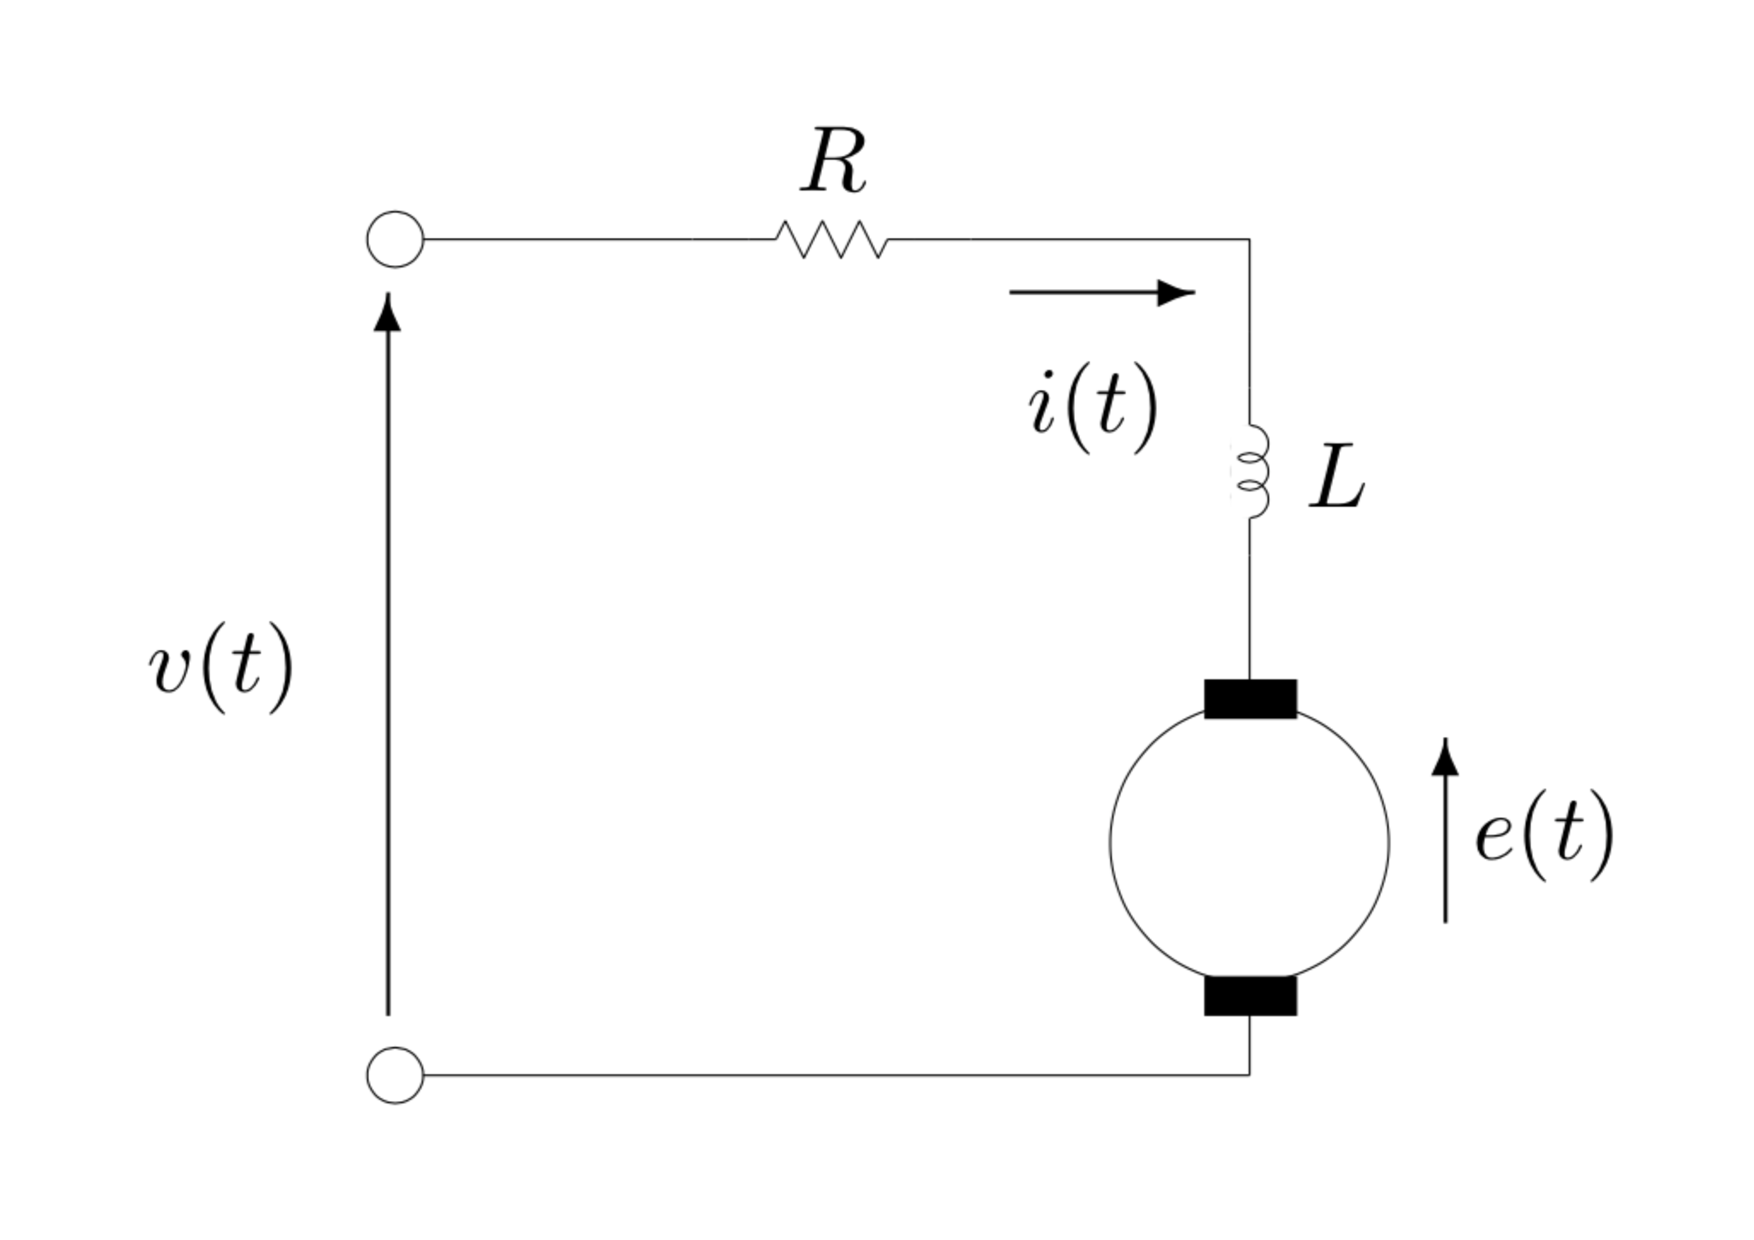
\includegraphics[width=12cm]{dc_eq.pdf}
    \caption{DCサーボモータの等価回路}
    \label{dc_eq}
\end{figure}


\begin{figure}[h]
    \centering
    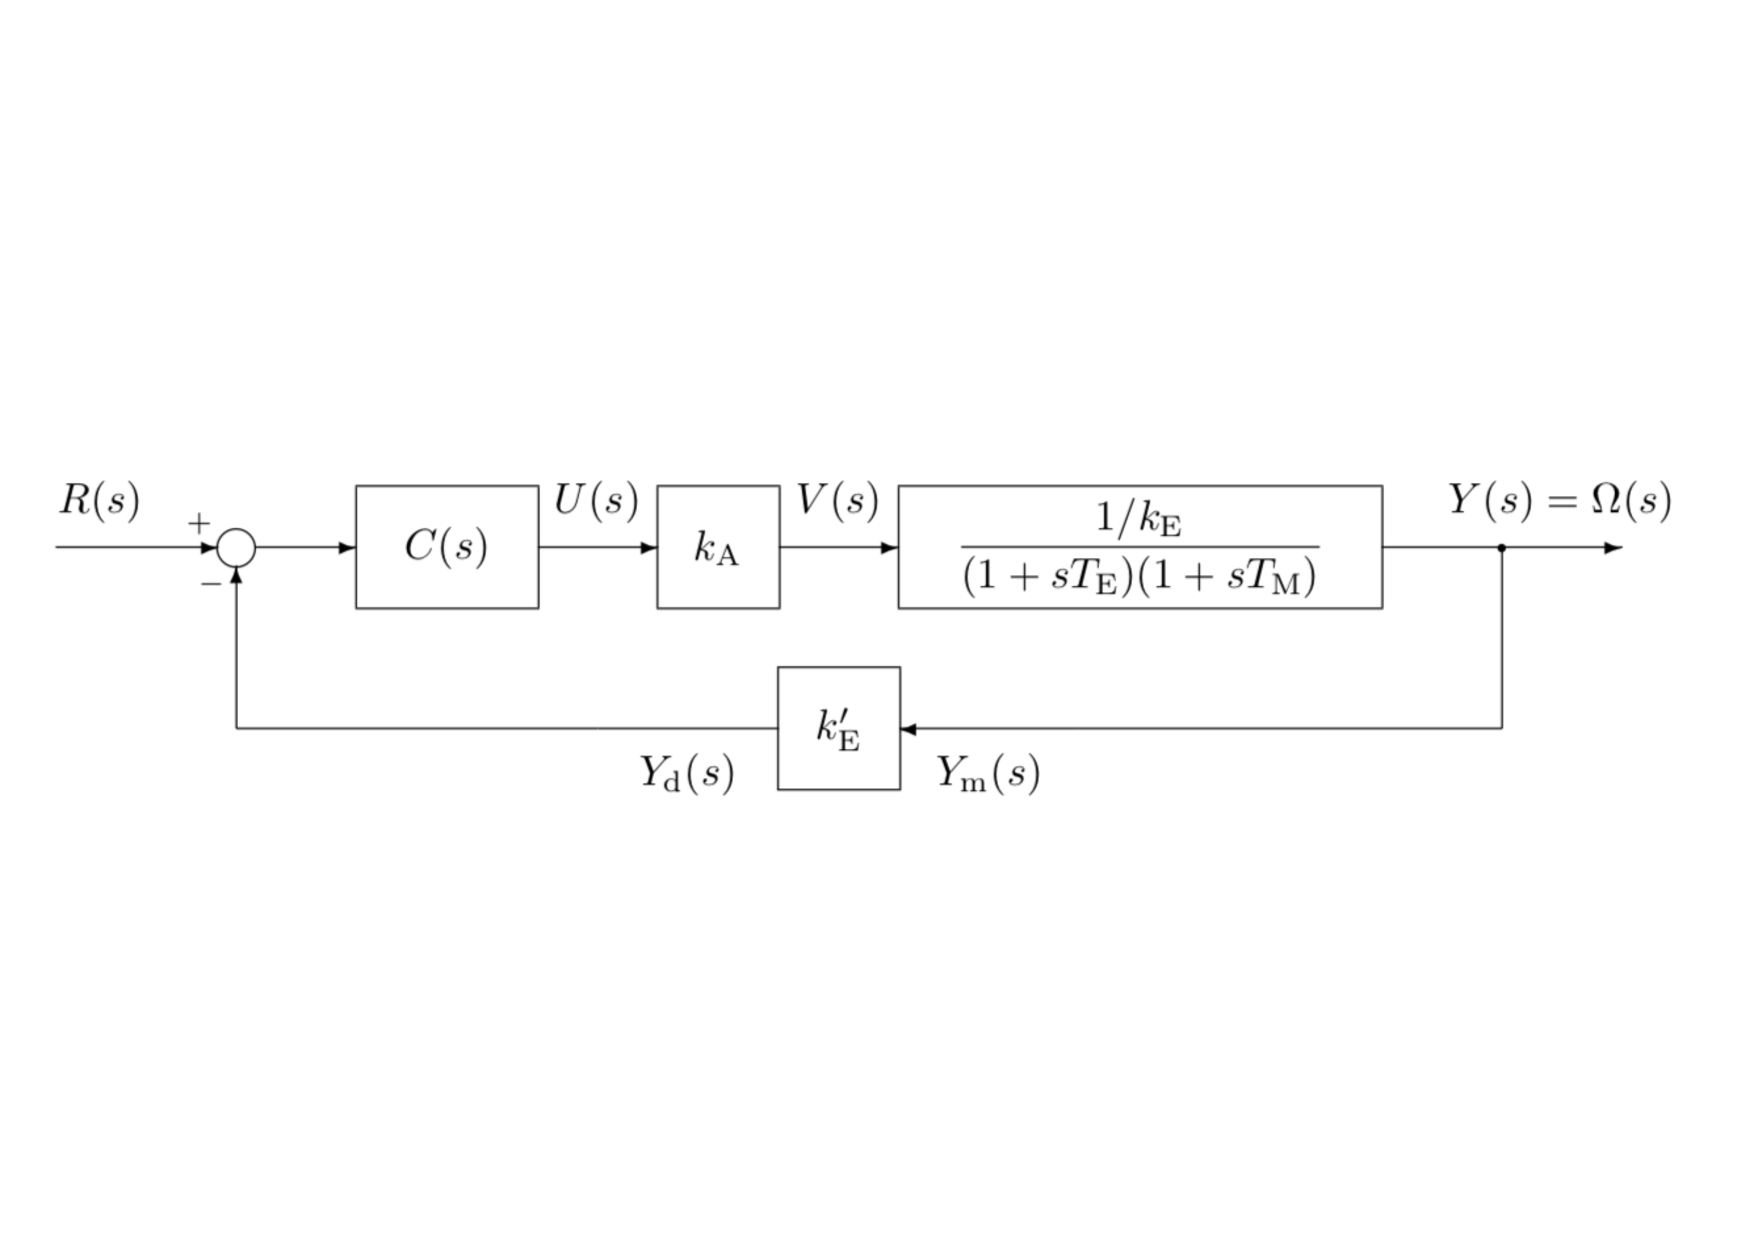
\includegraphics[width=12cm]{pv.pdf}
    \caption{速度制御のブロック線図}
    \label{pv}
\end{figure}

\begin{figure}[h]
    \centering
    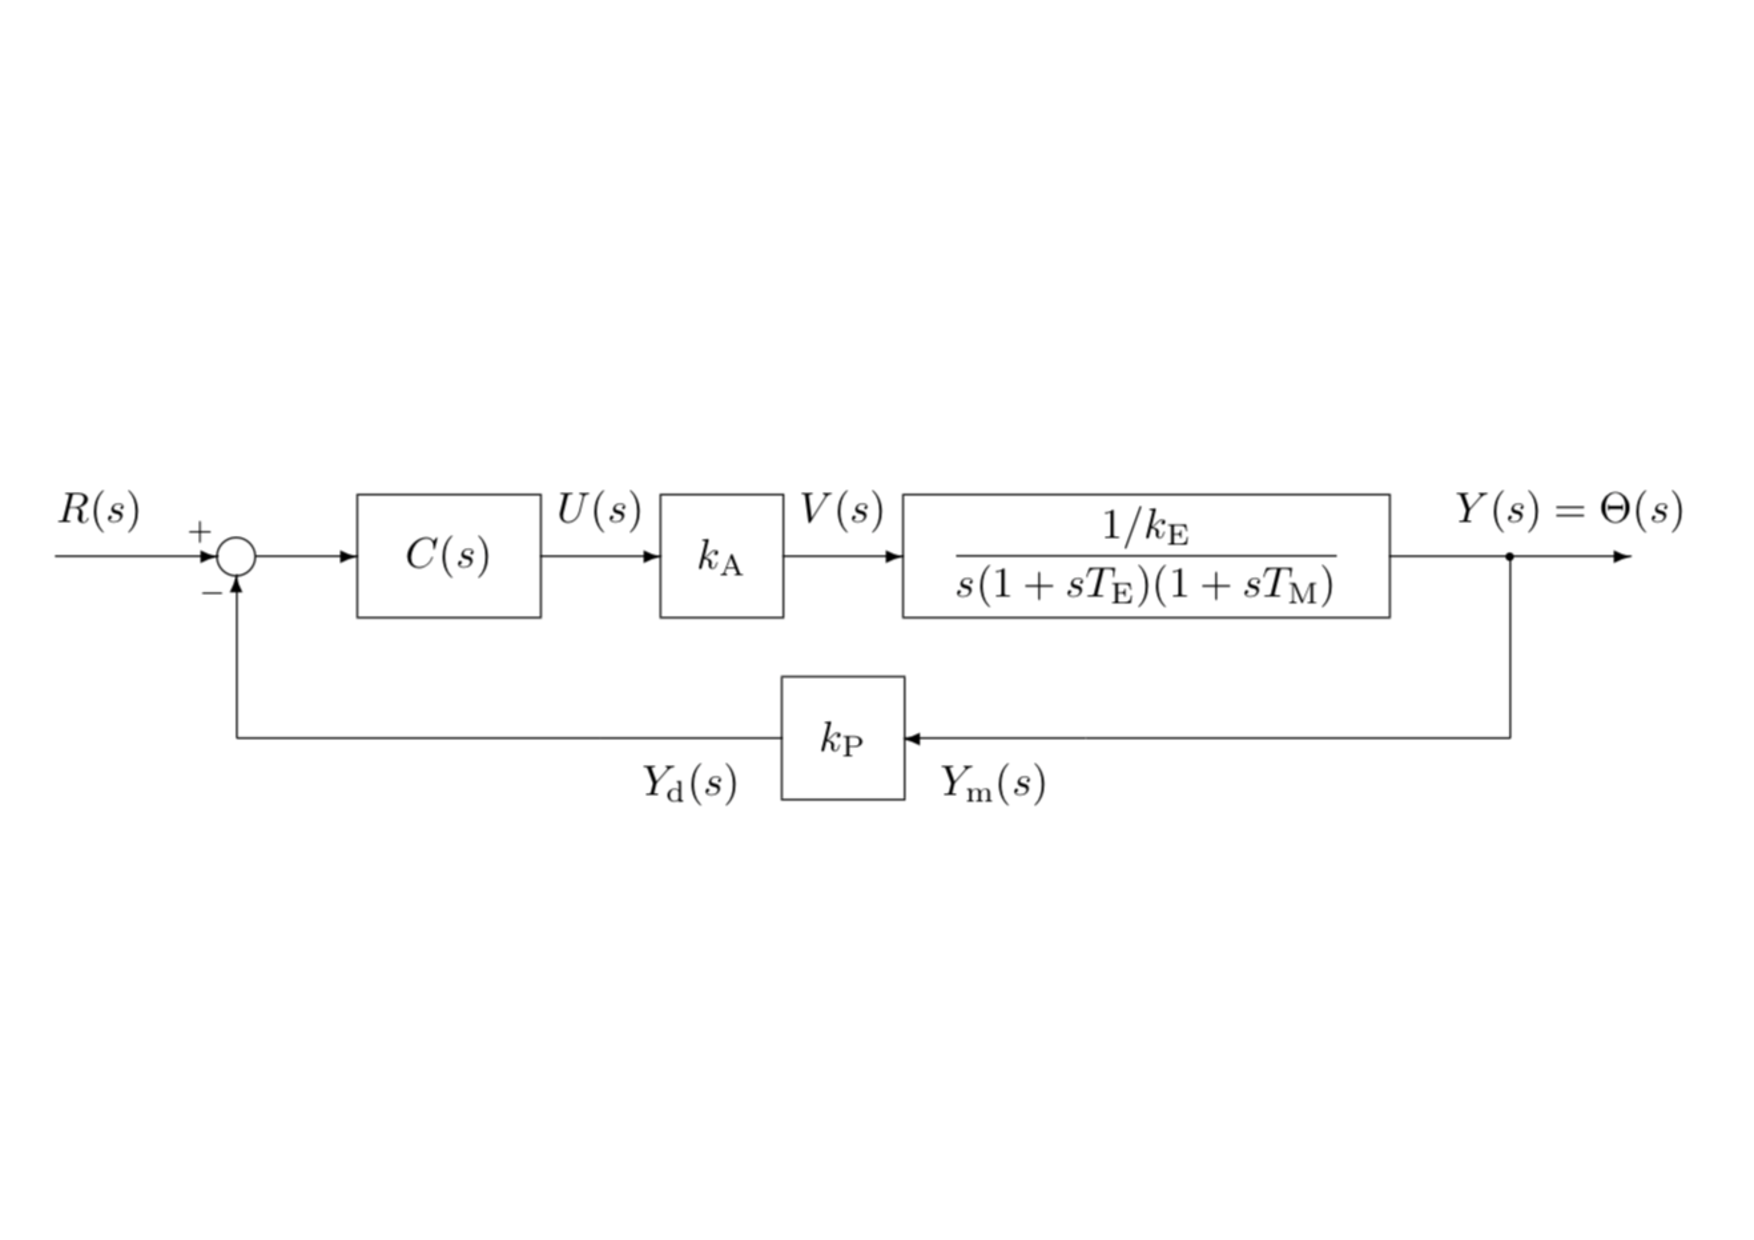
\includegraphics[width=12cm]{p.pdf}
    \caption{位置制御のブロック線図}
    \label{p}
\end{figure}

\newpage 
\ 
\newpage 
\section{方法}

今回用いた器具を以下に示す。

\begin{quote}
    \begin{itemize}
        \item ファンクションジェネレータ:Z94575
        \item オシロスコープ:IWATSU DS-5110 B
        \item 電源(小):KENWOOD PR18-1.2A
        \item 電源(大):TEXIO PS40-10A (Z000323513)
        \item ブレッドボード:5番
        \item DCサーボ:5番
        \item サーボモータドライバ:MS100T05
        \item ポテンショメータ:J40S
        \item カップリング:アサ電子工業製
        \item コンバータ:SUW3 0515
    \end{itemize}
\end{quote}

今実験に用いた装置構成図を図\ref{fig1}および図\ref{fig2}に示す。
図\ref{fig1}は速度制御を行うとき、
図\ref{fig2}は位置制御を行うときに用いた。

\newpage 

まず、速度制御を行った時の伝達関数$P_{V}(s)$の同定について説明する。

図\ref{fig1}のファンクションジェネレータの出力電圧を制御対象への入力、
タコジェネレータの出力電圧を制御対象からの出力とみなして、
入力周波数を0.2${\rm Hz}$から100${\rm Hz}$の間で20点ほど
変化させながら電圧をオシロスコープで計測した。
ここで、制御対象の入力、出力とみなしたところはそれぞれ図\ref{pv}における
$C(s)$への入力信号、$Y_{\rm d}(s)$とみなせる。

次に、位置制御を行った時の伝達関数$P(s)$の同定について説明する。

図\ref{p}のファンクションジェネレータの出力電圧を制御対象への入力、
ポテンショメータの出力電圧を制御対象からの出力とみなして、
入力周波数を2${\rm Hz}$から20${\rm Hz}$の間で6点ほど
変化させながら電圧をオシロスコープで計測した。
ここで、制御対象の入力、出力とみなしたところはそれぞれ図\ref{p}における
$C(s)$への入力信号、$Y_{\rm d}(s)$とみなせる。

それぞれの計測結果からボード線図を描き、伝達関数を同定する。

\begin{figure}[h]
    \centering
    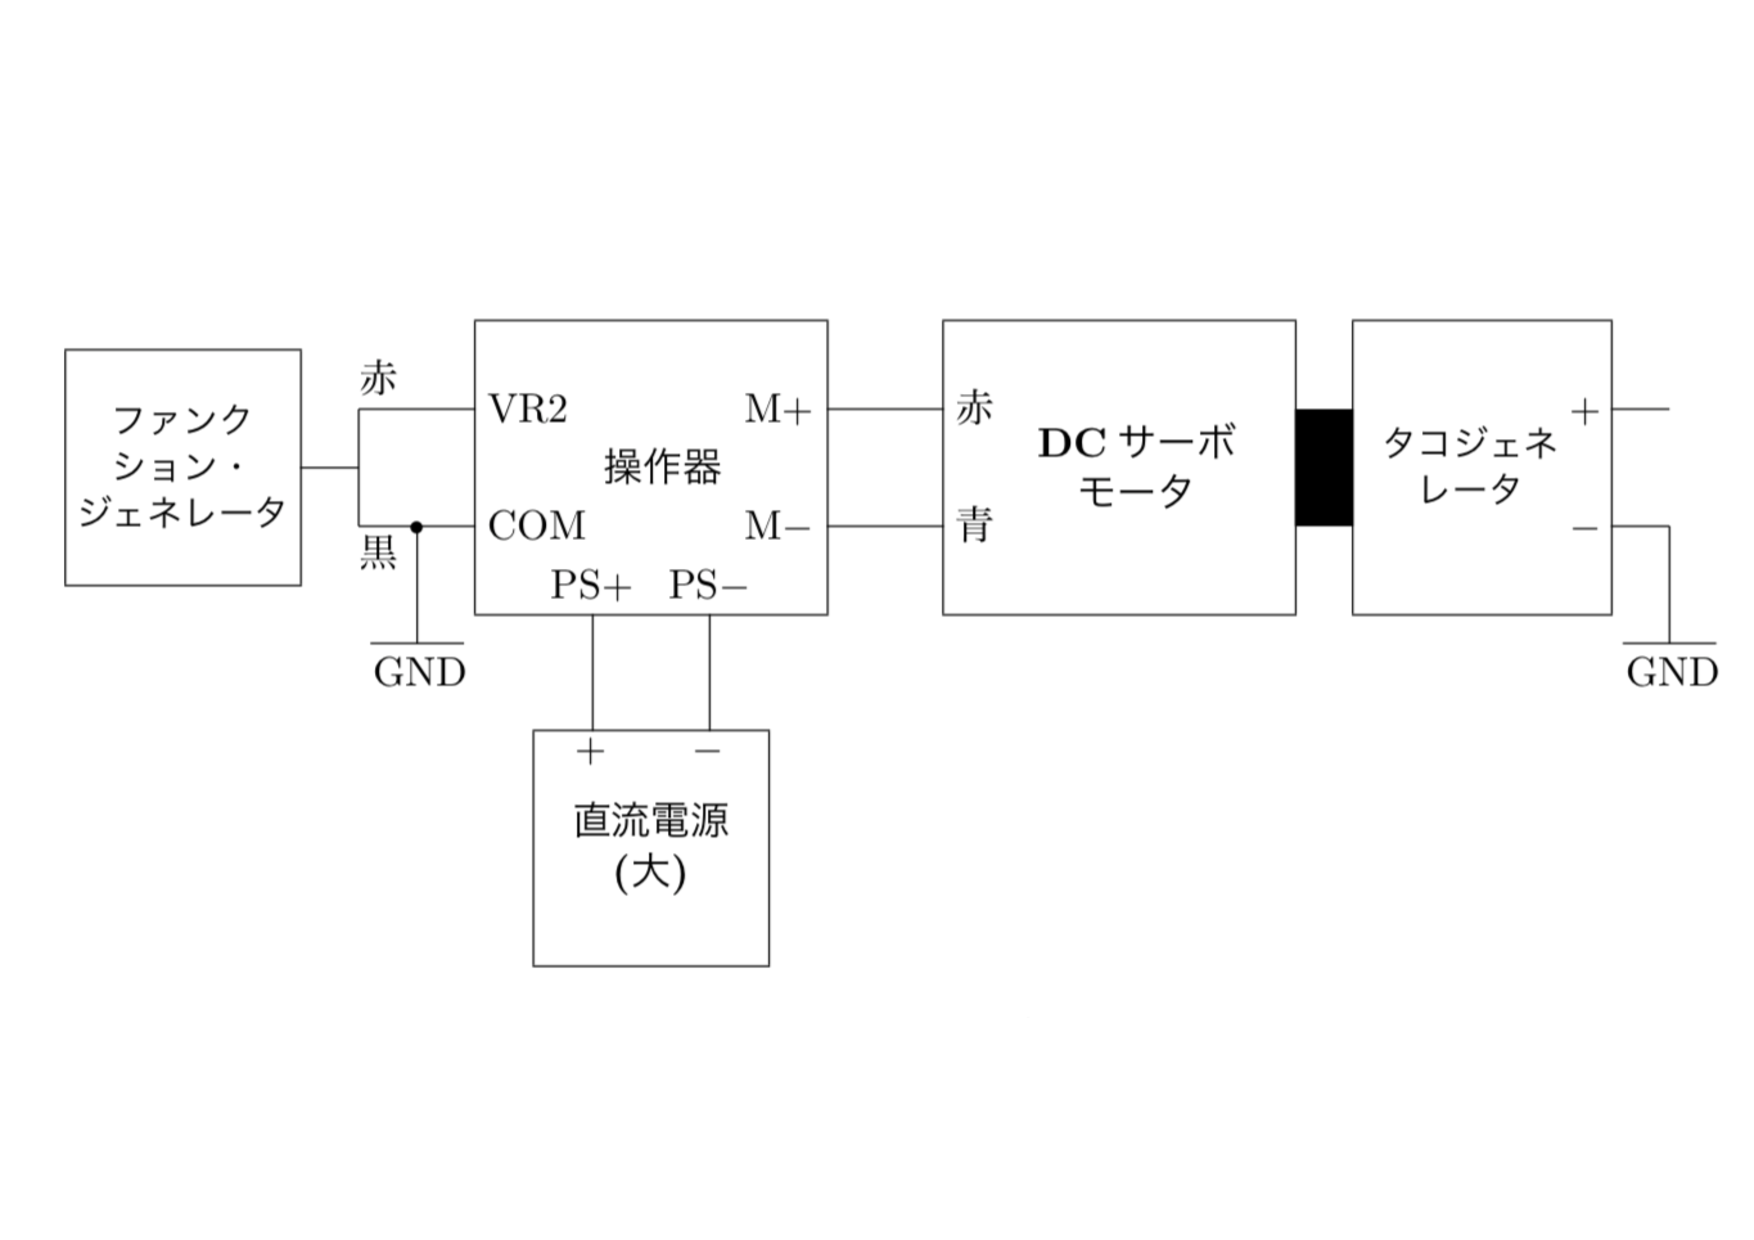
\includegraphics[width=12cm]{fig1.pdf}
    \caption{実験1-1の装置構成図}
    \label{fig1}
\end{figure}

\begin{figure}[h]
    \centering
    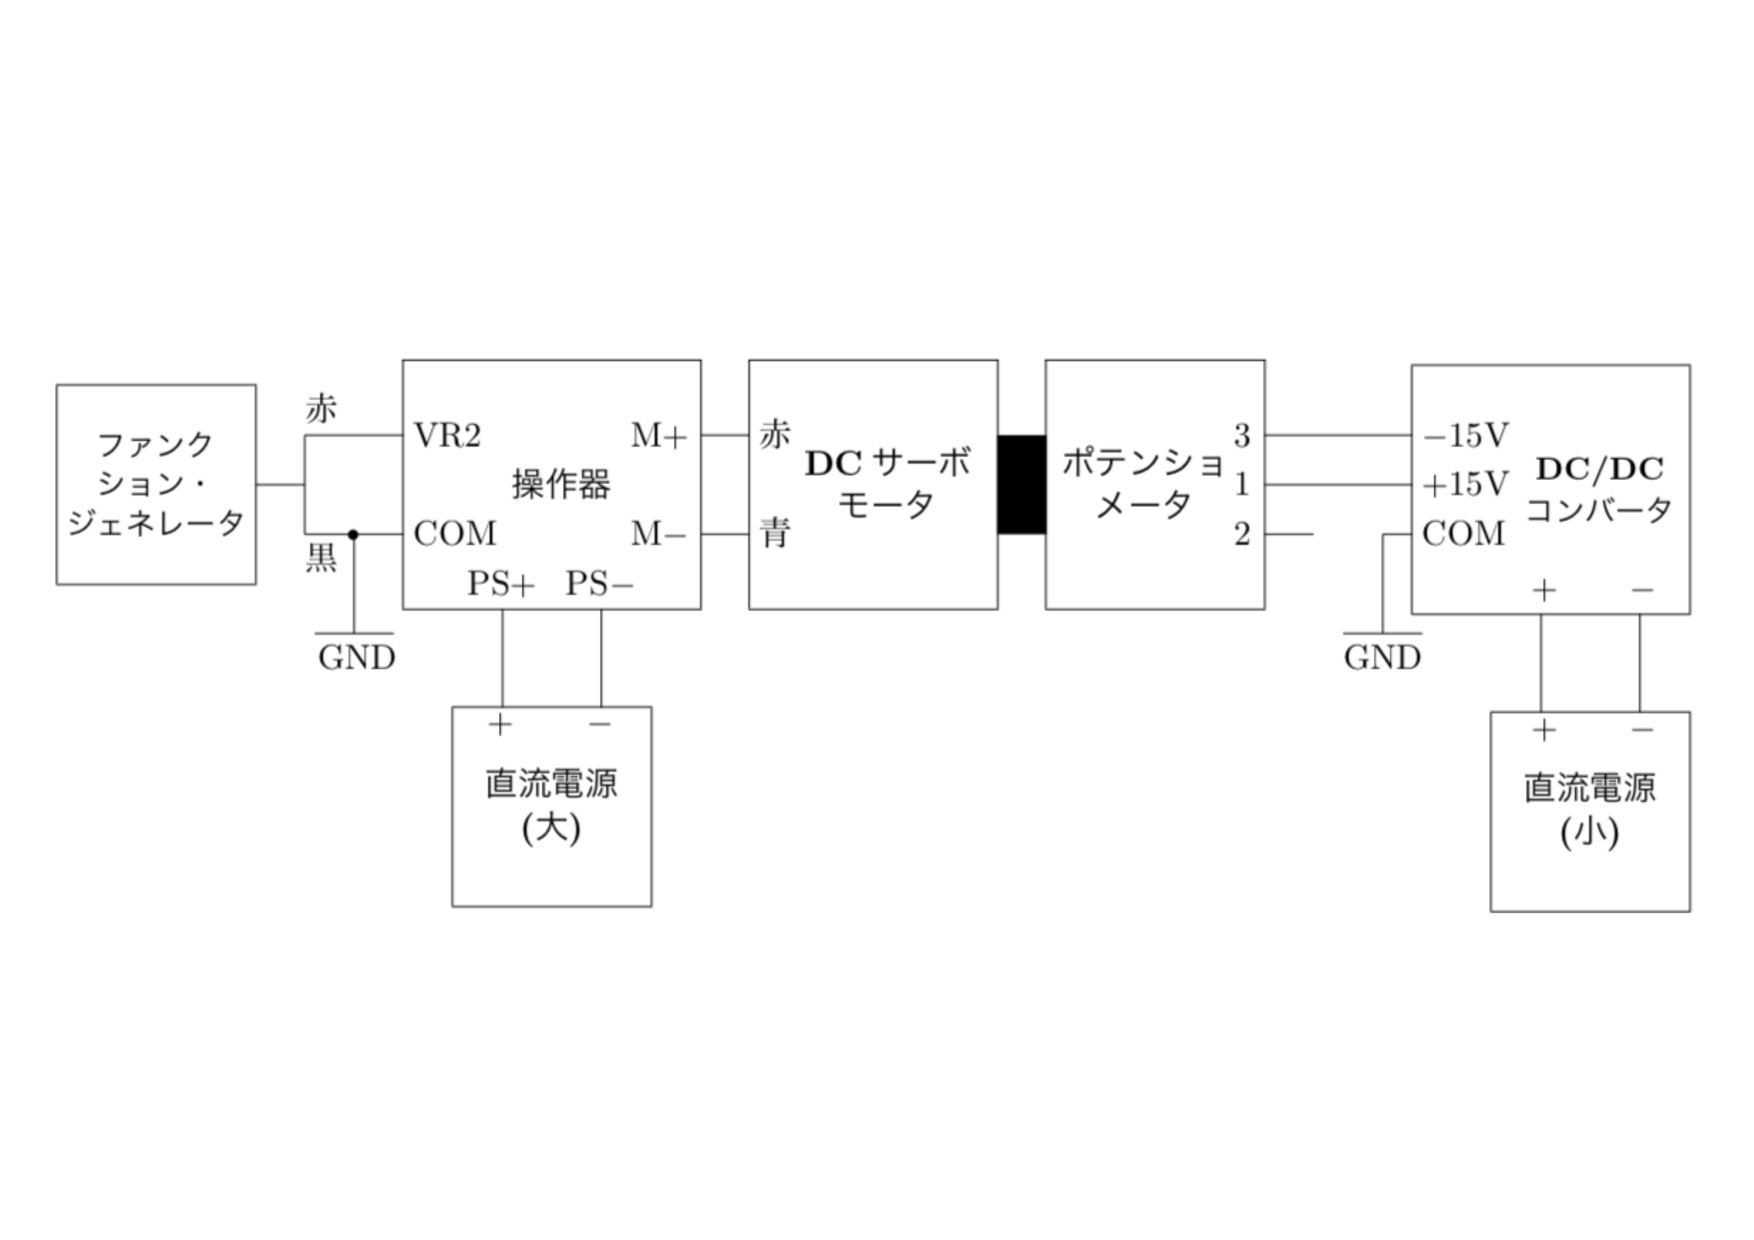
\includegraphics[width=12cm]{fig2.pdf}
    \caption{実験1-2の装置構成図}
    \label{fig2}
\end{figure}

\newpage

\section{実験結果}

位置制御によって得られたデータは、式\ref{twentythree}、
\ref{twentyfour}を元に得られる関係式

\begin{equation}\label{twentyfive}
    P(s)=\frac{k_{\rm P}}{sk'_{\rm E}}P_{\rm V}(s)
\end{equation}

から得られる変換式

\begin{equation}\label{twentyfive'}
    |P_{\rm V}| = \frac{\omega k'_{\rm E}}{k_{\rm P}}|P|
\end{equation}

\begin{equation}\label{twentyfive''}
    {\rm arg}P_{\rm V} = {\rm arg}P + 90
\end{equation}

を用いて位相制御の計測値を速度制御のものと同様に扱えるように変換し、
ボード線図を描いたものを図\ref{bode}に示す。

% \begin{table}\label{table_pv}
%     \begin{tabular}{|l|r|r|r|r|}\hline
%         周波数[${\rm Hx}$] & 入力振幅[{\rm V}] & 出力振幅[{\rm V}]
%         & ゲイン & 位相差[度] \\ \hline
%     \end{tabular}
% \end{table}

\begin{figure}[h]
    \centering
    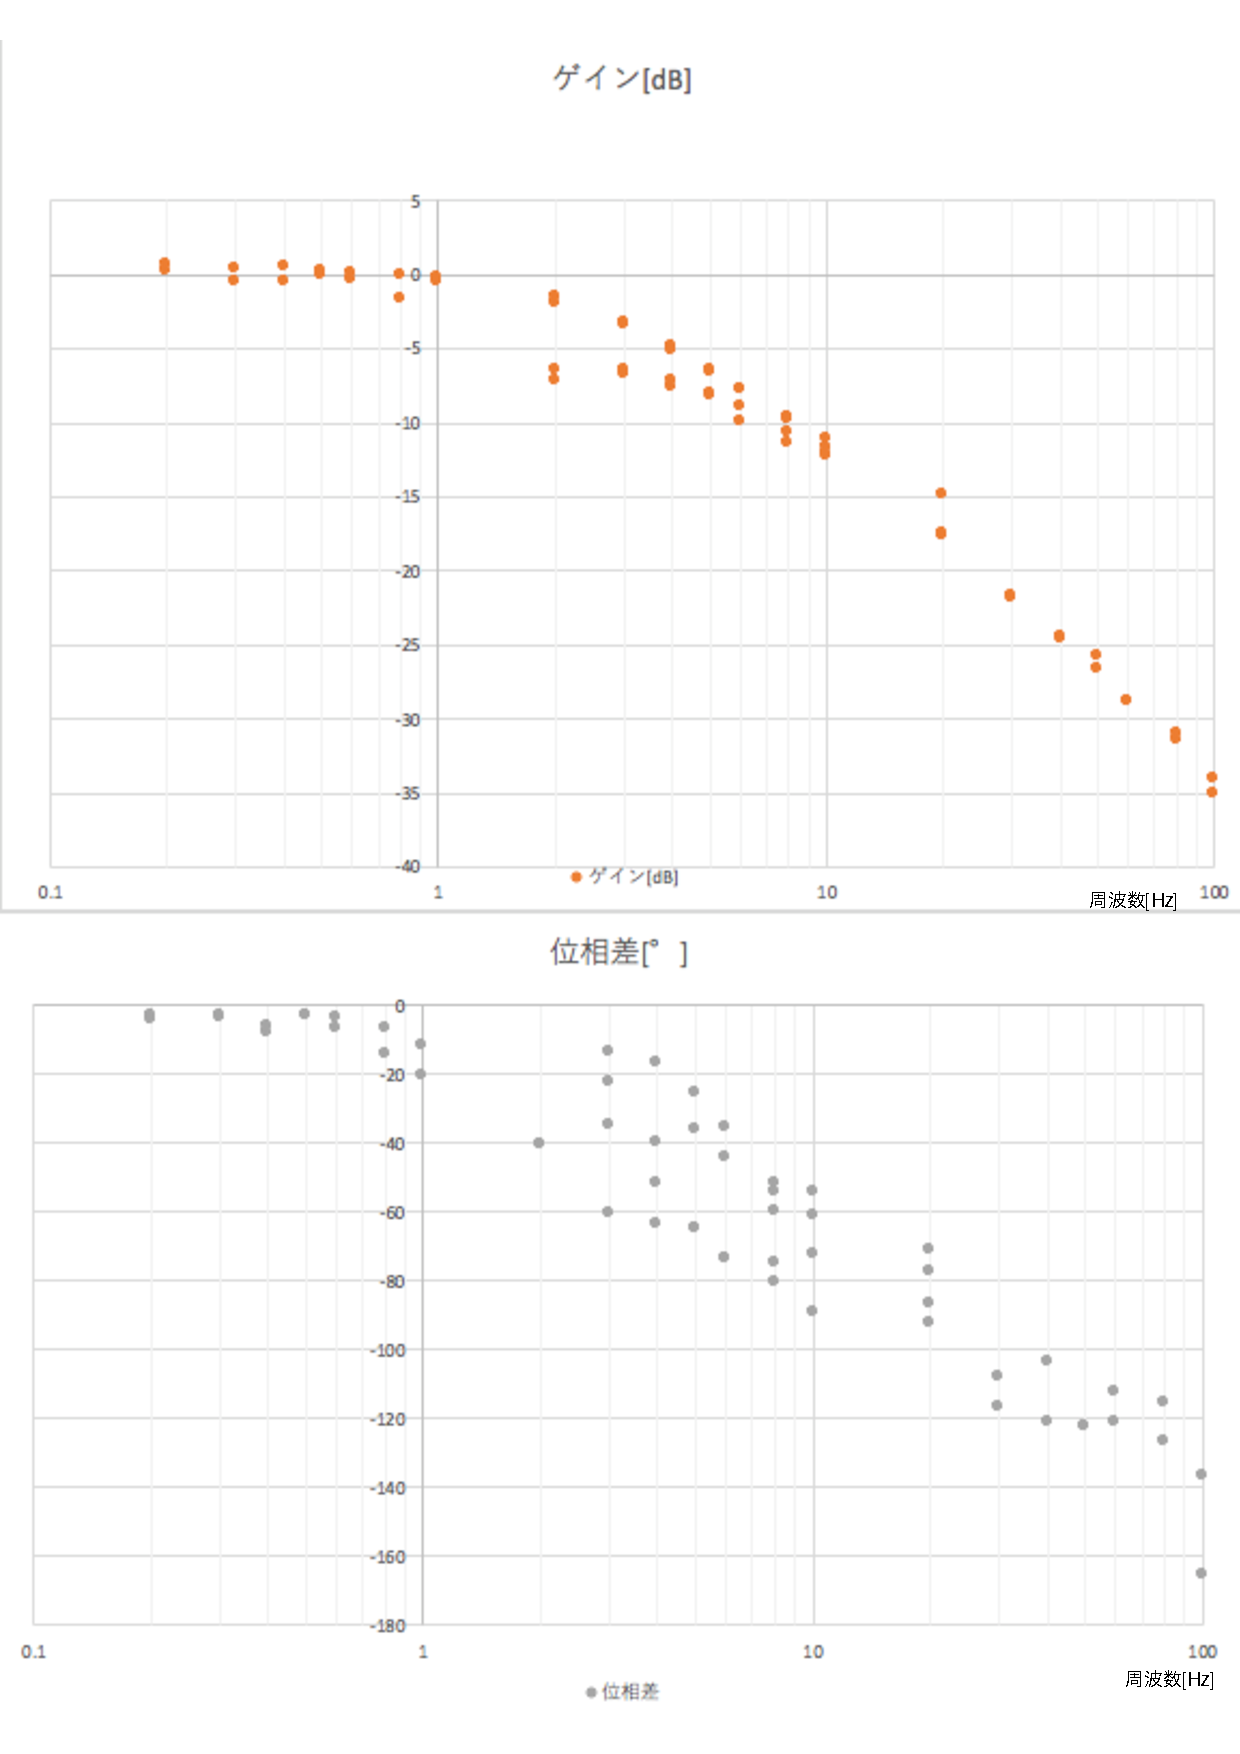
\includegraphics[width=10cm]{bode.pdf}
    \caption{制御対象のボード線図}
    \label{bode}
\end{figure}

\newpage

\section{考察}

まず、1回転ポテンショメータに対する$k_{\rm p}$の値を考える。
ポテンショメータの両端子にはそれぞれ-15Vと15Vの電源を接続した。
1回転ポテンショメータは1回転する間に-15Vから15Vへ変化するので、
式\ref{eighteen}を参考に考えると$k_{\rm p}$の値は30/2$\pi$に
なると考えた。

\newpage

次に逆起電力定数$k'_{\rm E}$の算出法について考える。

1回転ポテンショメータをDCサーボモータに取り付けた状態で、
DCサーボモータ・ドライバに一定の直流電圧を与えて
DCサーボモータを定速回転させ、
この状態でのタコジェネレータ及びポテンショメータの出力電圧波形を
観測することによっても測定できる。
その原理は、式\ref{twentythree}、\ref{twentyfour}を参照して
考えると、与えられた状況下では$P(s)$と$P_{\rm V}(s)$の差異が生じるのは
それぞれの定数$k_{\rm A}$、$k'_{\rm E}$によってだけである。
したがってそれぞれの出力電圧波形の比をとると$k_{\rm A}$/$k'_{\rm E}$
が求まるので、そこに$k_{\rm A}$を代入すれば$k'_{\rm E}$が求まる。

最後に、$K$、$T_{\rm E}$、$T_{\rm M}$の同定を行った。
まず、ボード線図の理論的な概形を考える。

式\ref{twentythree}を参考に理論的なボード線図の概形を描いたものが、
図\ref{ideal_bode}に示す。
これは、一次遅れのボード線図を元に考えた。
これを元に、図\ref{bode}の特にゲインの方を使いそれぞれに値を同定した。
実際の同定には、グラフを印刷して線を引いて求めた。
求めた値はそれぞれ

\begin{equation}
    K=1.03
\end{equation}

\begin{equation}
    T_{\rm M} = 0.0909
\end{equation}

\begin{equation}
    T_{\rm E} = 0.00132
\end{equation}

となった。実際この値を用いて求めたグラフを実測値を元にしたグラフに重ねると
図\ref{ideal_real}、\ref{ideal_real2}のようになる。
高周波部分は補助線が引きづらかったため、特に$T_{\rm E}$の値の推定が
難しく、その結果がゲイン図の高周波域での実測値とのズレが出たのだと考えた。


以後は値が必要になった時はこの値を用いることにする。

\begin{figure}[h]
    \centering
    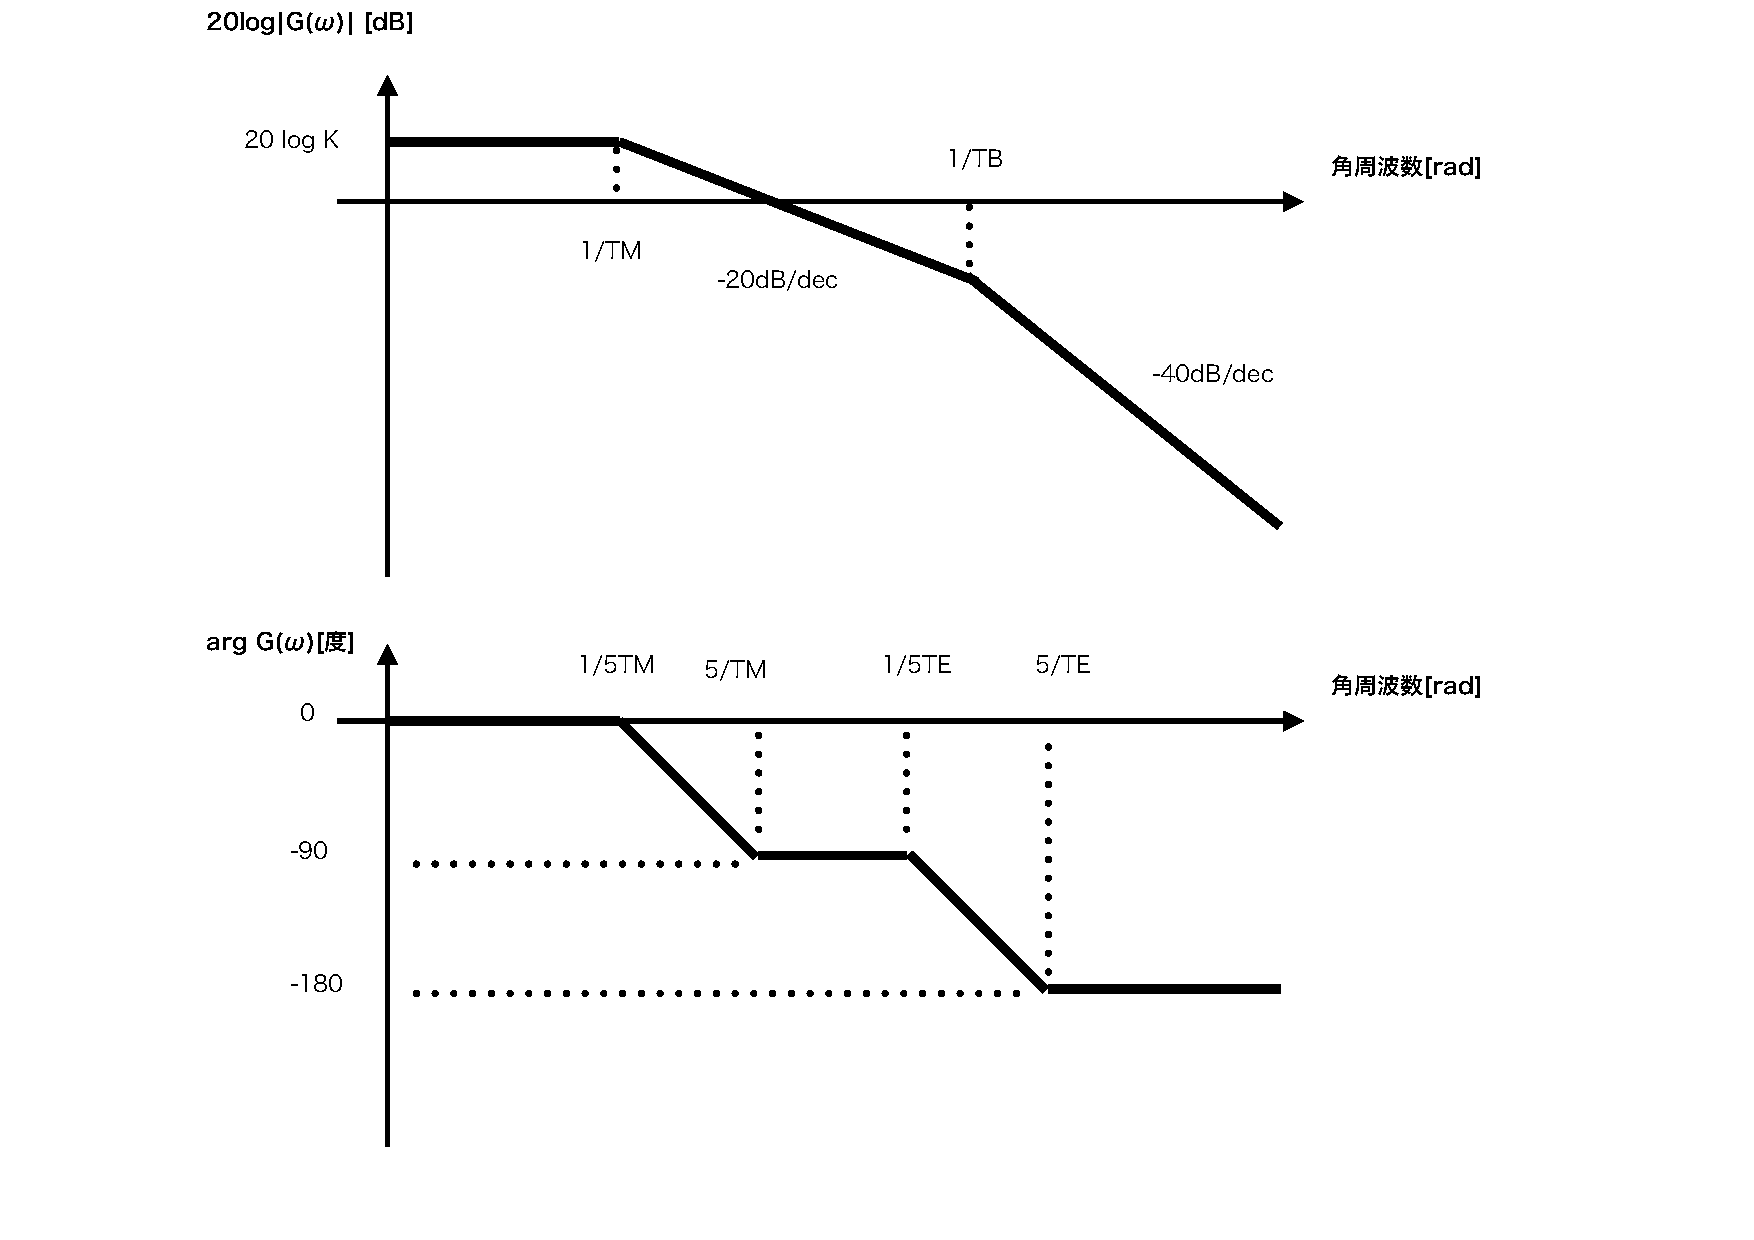
\includegraphics[width=12cm]{ideal_bode.pdf}
    \caption{理論的なボード線図}
    \label{ideal_bode}
\end{figure}

\begin{figure}[h]
    \centering
    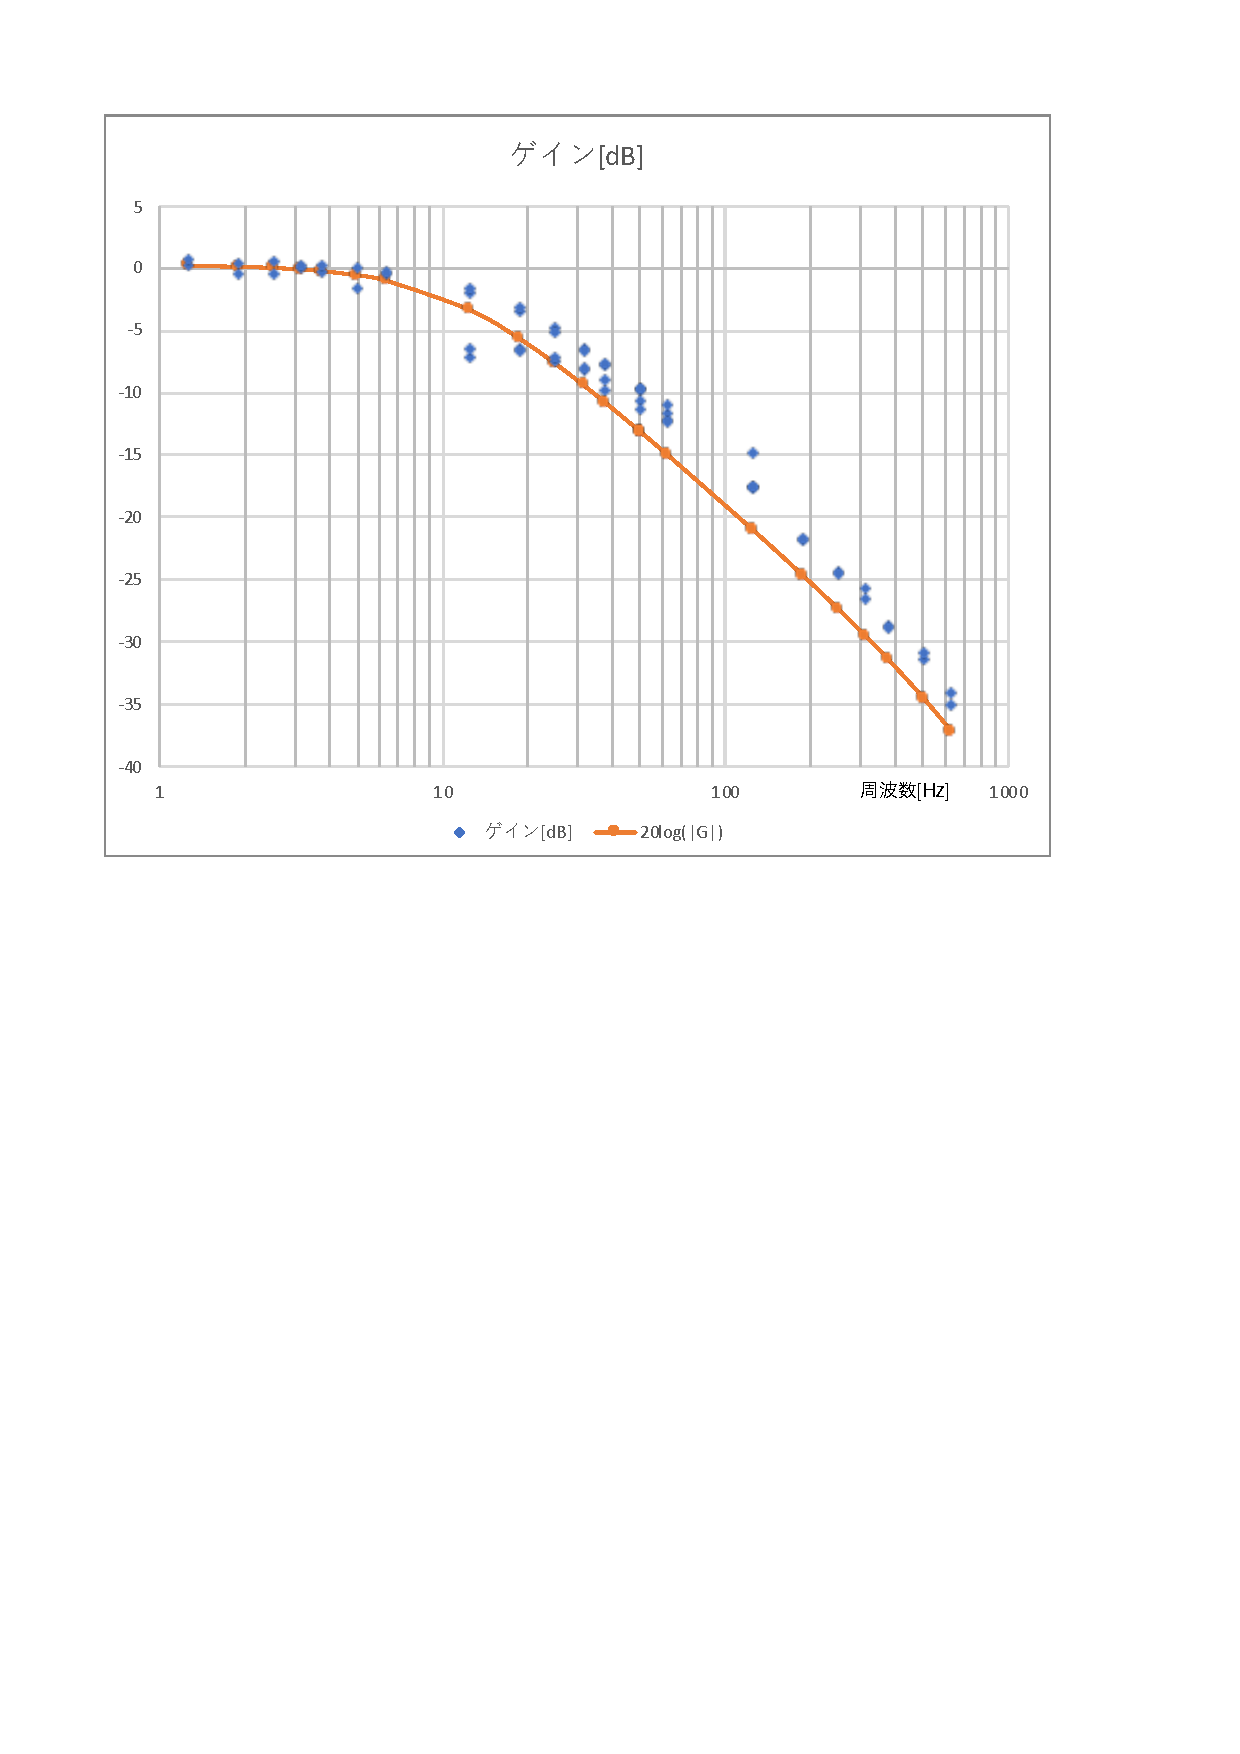
\includegraphics[width=9cm]{ideal_real.pdf}
    \caption{推測値と実測値}
    \label{ideal_real}
\end{figure}


\begin{figure}[h]
    \centering
    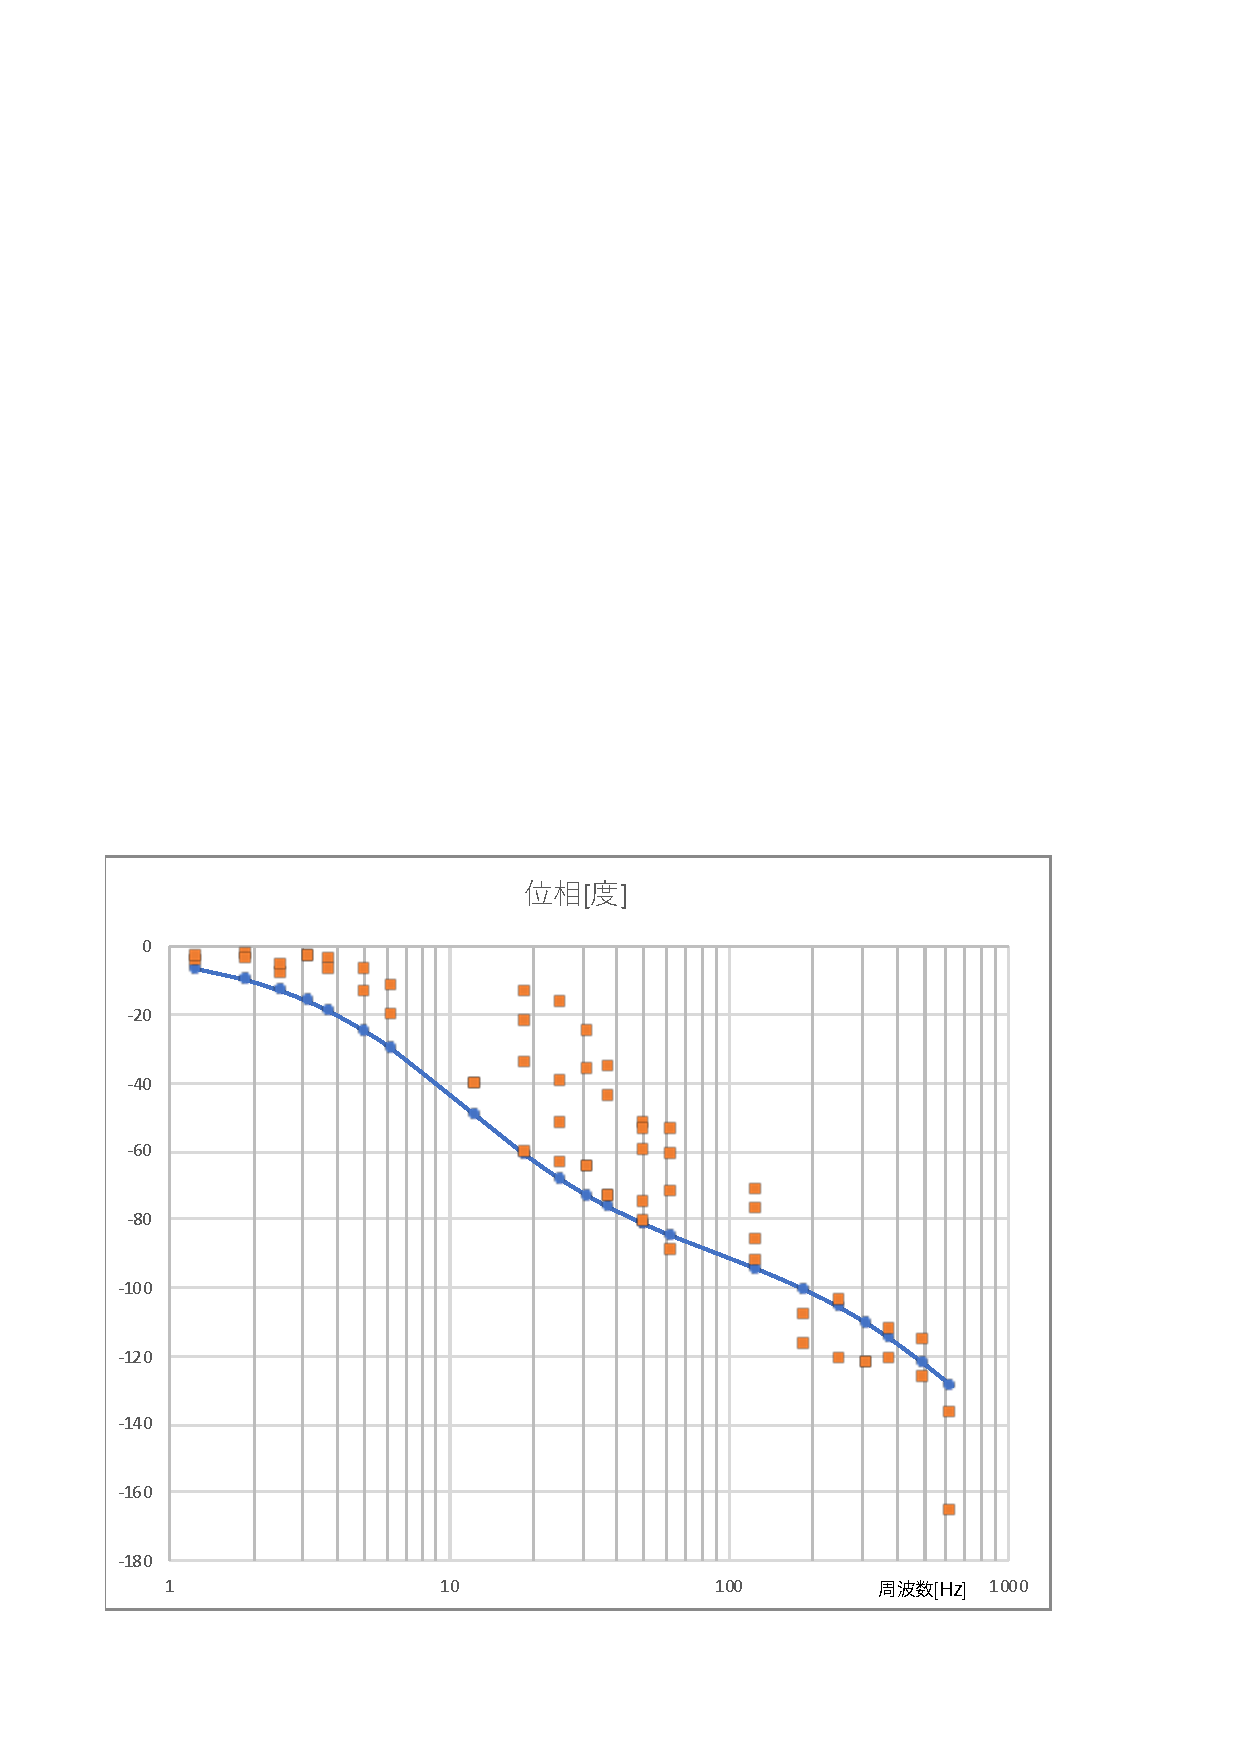
\includegraphics[width=9cm]{ideal_real2.pdf}
    \caption{推測値と実測値2}
    \label{ideal_real2}
\end{figure}
% K,Te,Tm
% ideal bode

% 実験レポート1
% ここまで

\newpage
\newpage
\ 
\newpage
\ 
\newpage

% 実験レポート2
% ここから

% \subtitle{2020/11/6}

\theme{実験2}
\section{目的}
制御用アナログ回路を作成しそれを各制御に用いて測定する。
その結果を測定し、安定性や定常偏差、応答について議論する。

\section{原理}
今実験では、制御用アナログ回路は図\ref{a}および\ref{b}に示す構成の
ものを使用する。

まず、図\ref{a}において、

\begin{equation}\label{twenty_seven}
    v_{\rm out}(t) = K_{\rm C}(v_{\rm ref}(t) - v_{\rm in}(t))
\end{equation}

の関係が成り立つ。この式を導出する。

オペアンプの+での電圧を$V_+$、-での電圧を$V_-$とすると、

% \begin{equation}
    % v_{\rm in} = \frac{R_2}{R_2 + R_1}v_{\rm ref}
% \end{equation}

\begin{equation}
    \frac{v_{\rm in} - V_-}{R_1} = \frac{V_- - v_{\rm out}}{R_2}
\end{equation}

\begin{equation}
    V_+ = \frac{R_2}{R_1+R_2}v_{\rm ref}
\end{equation}

が成立し、仮想短絡のことを考えると$V_+=V_-$が成立するので、

\begin{equation}\label{twenty_seven}
    v_{\rm out}(t) = \frac{R_2}{R_1}(v_{\rm ref}(t) - v_{\rm in}(t))
\end{equation}

が得られる。したがって$K_C = \frac{R_2}{R_1}$が得られる。

次に、図\ref{b}において

\begin{equation}\label{thirty}
    C(s)=K_C\frac{\alpha (1+sT)}{1+s\alpha T}
\end{equation}

が成立する。

この式を導出する。
まず回路の左側は\ref{a}と同じなので、図中の境目では

\begin{equation}
    V_X = - \frac{R_2}{R_1}(V_{\rm in} - V_{\rm ref})
\end{equation}

となる。オペアンプの仮想短絡を考えると、

\begin{equation}
    \frac{V_X}{\frac{R_3}{1+sC_1}} 
        = \frac{V_{\rm out}}{\frac{R_4}{1+sC_2}}
\end{equation}

となるので、これを変形して

\begin{equation}
    C(s) = \frac{R_2R_4}{R_1R_3}\frac{1+sC_1R_3}{1+sC_2R_4} 
    = \frac{C_2R_2}{C_1R_1} 
    \frac{\frac{C_2R_4}{C_1R_3}(1+sC_1R_3)}{1+s\frac{C_2R_4}{C_1R_3}C_1R_3}
\end{equation}

したがって

\begin{equation}
    K_C =\frac{C_2R_2}{C_1R_1} 
\end{equation}

\begin{equation}
    \alpha =\frac{C_2R_4}{C_1R_3} 
\end{equation}

\begin{equation}
    T=C_1R_3
\end{equation}

が算出できる。

\begin{figure}[h]
    \centering
    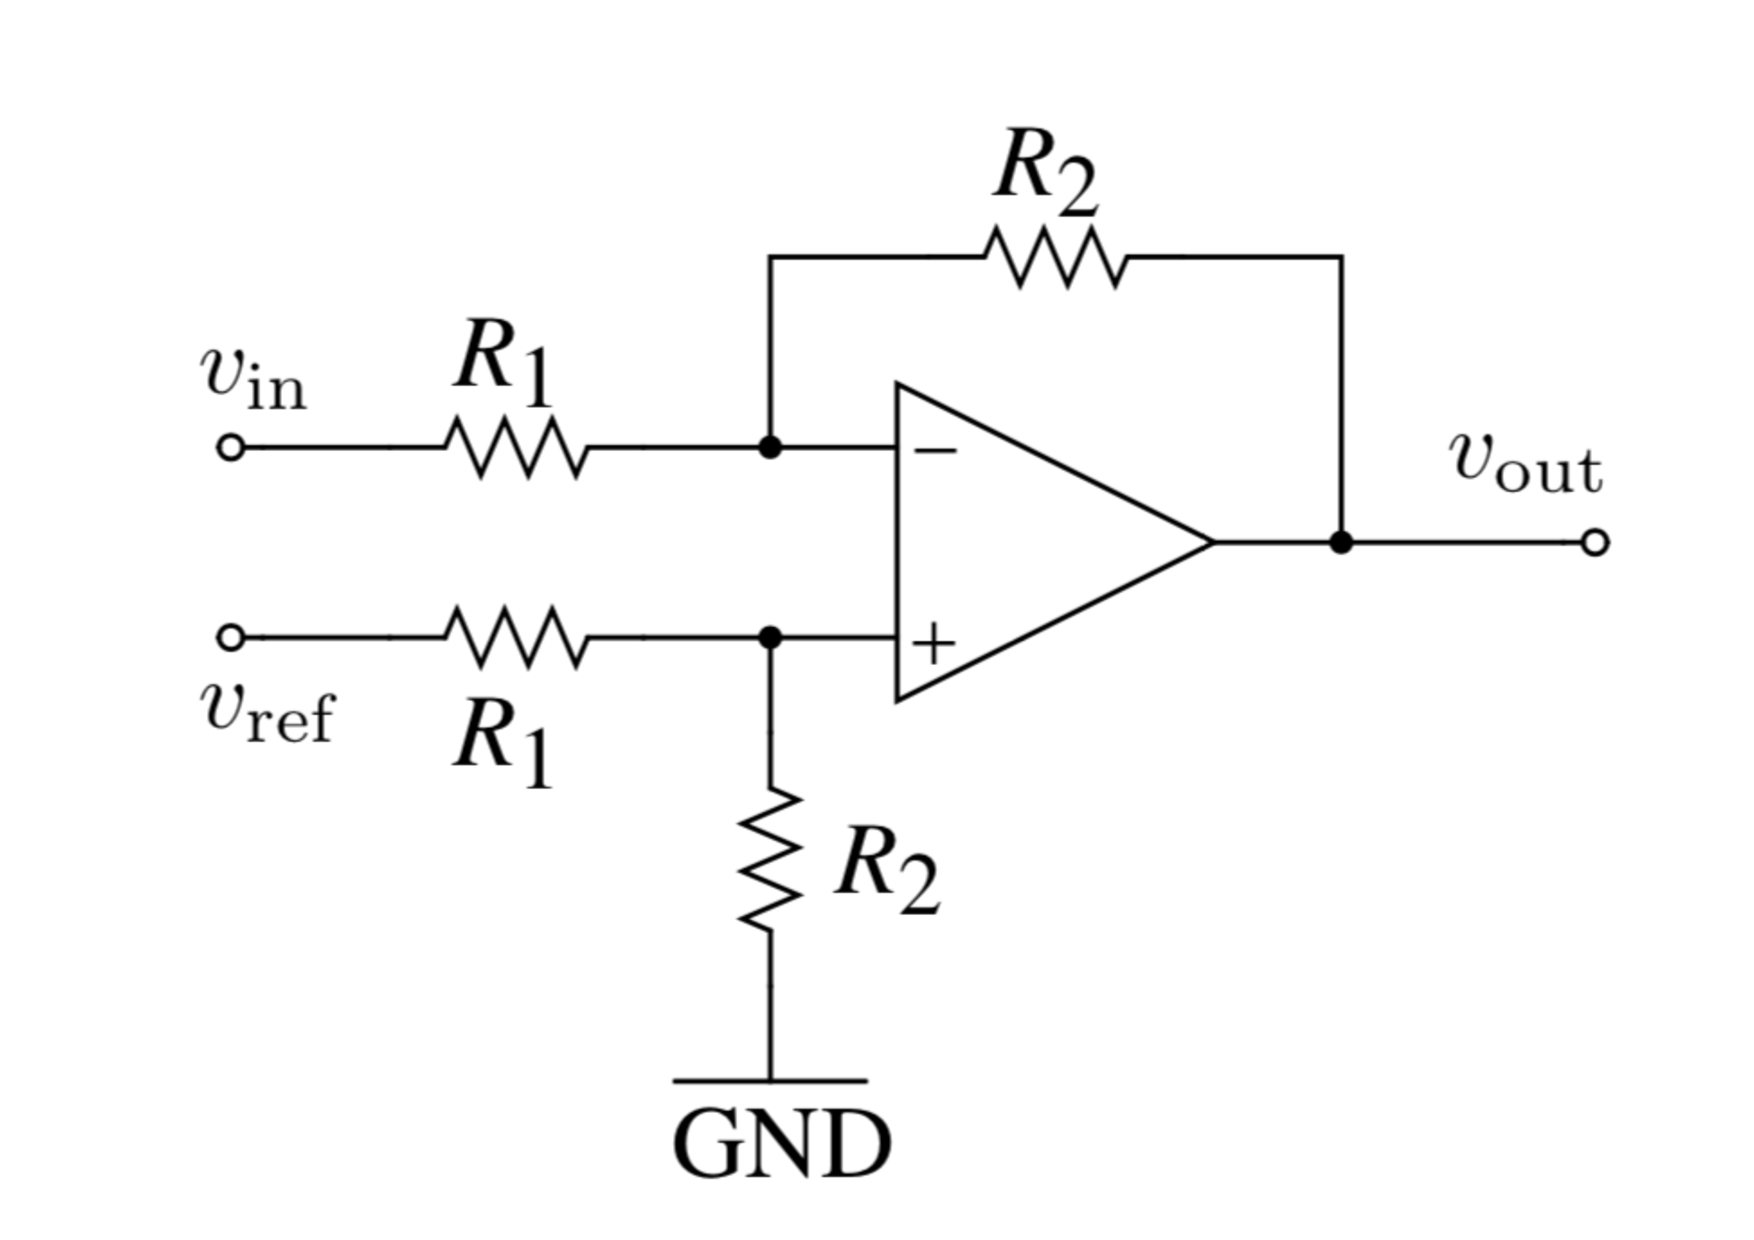
\includegraphics[width=12cm]{a.pdf}
    \caption{制御用アナログ回路(a)}
    \label{a}
\end{figure}

\begin{figure}[h]
    \centering
    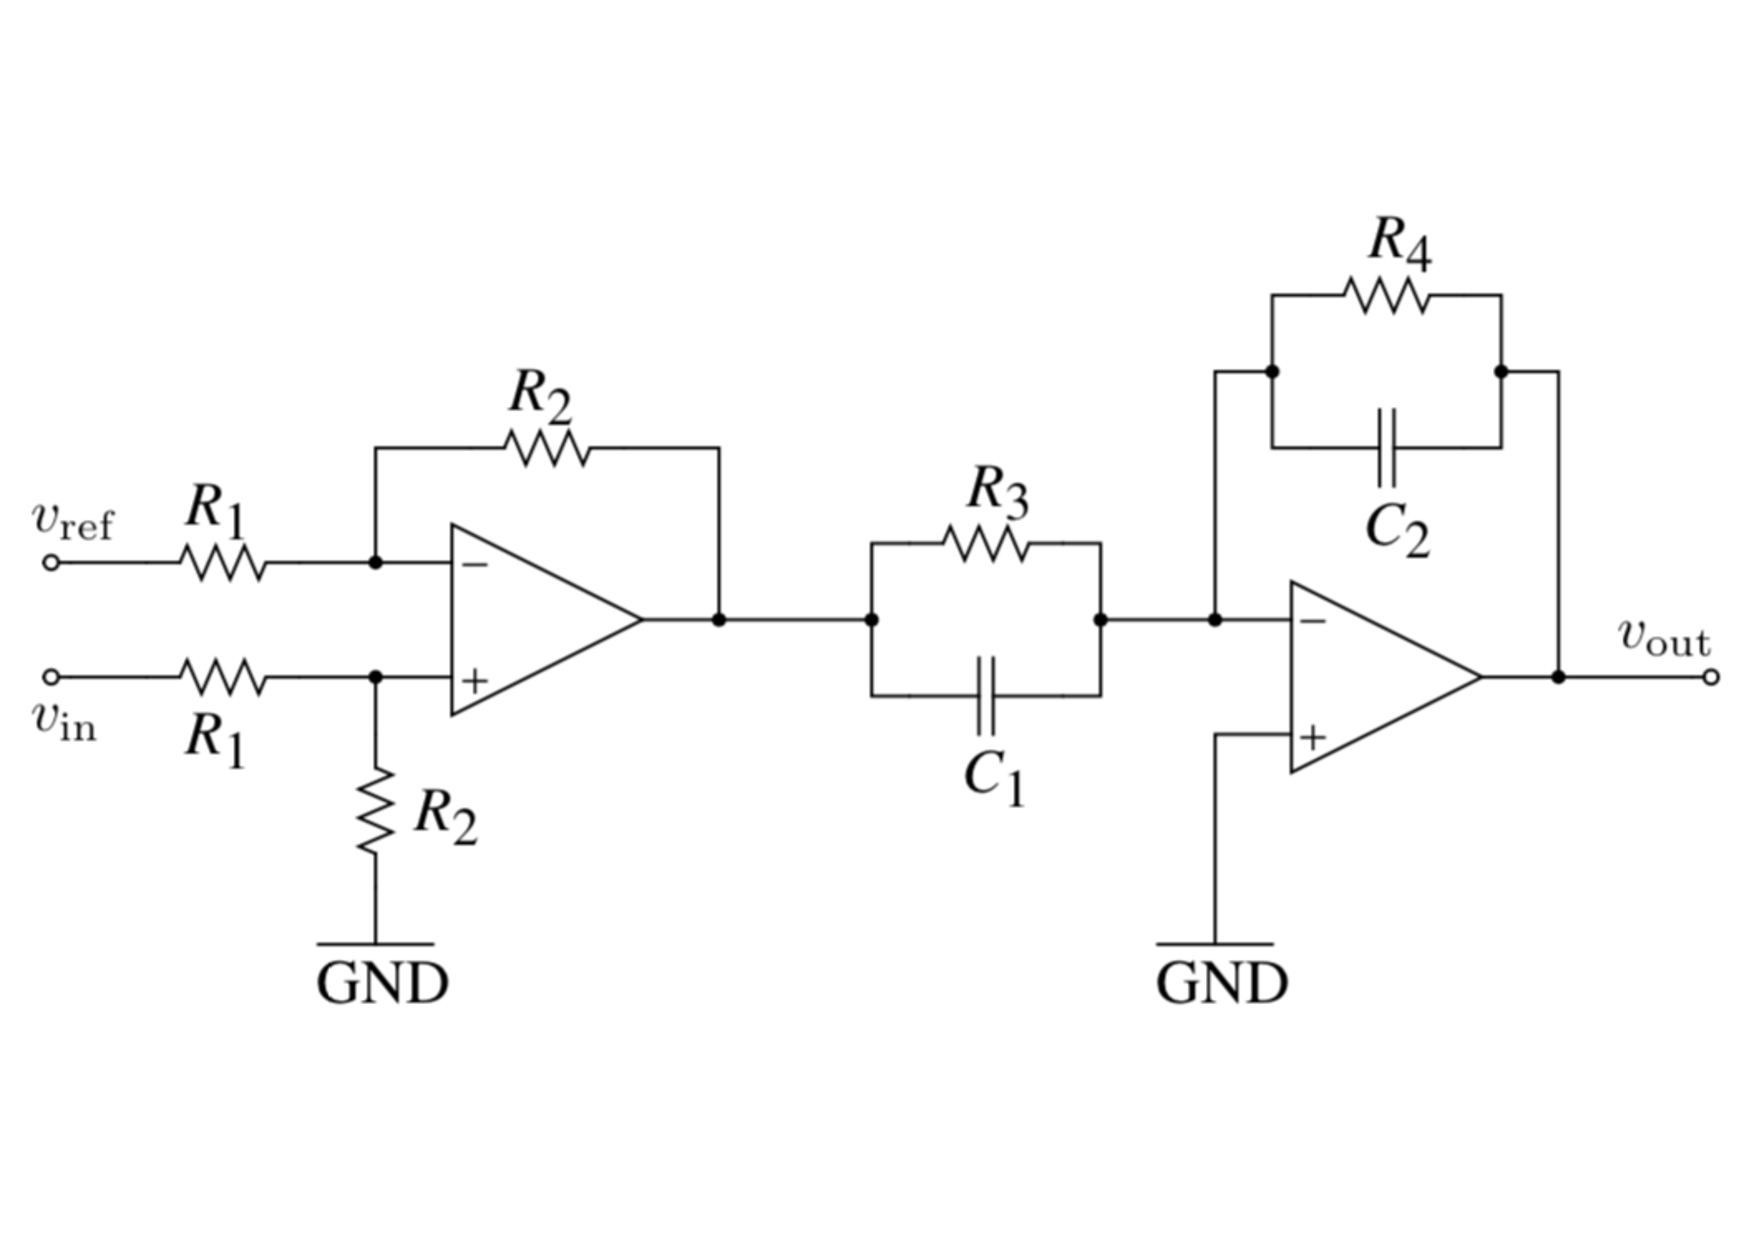
\includegraphics[width=12cm]{b.pdf}
    \caption{制御用アナログ回路(b)}
    \label{b}
\end{figure}

\newpage

\section{実験}

上で示した制御回路(a)、(b)を用いて
周波数特性を測定し、
そのボード線図を書く。
制御回路は上の回路図を参考に回路を組み、
全体の測定装置は図\ref{souchi2}のように組んだ。
そして周波数を0.2~500Hzまで変化させながら周波数特性を測定した。

なお、回路に用いた素子は(a)の測定装置では$R_1=20{\rm k \Omega}$、
$R_2=300{\rm k \Omega}$を用いた。また、(b)においては
$R_1=470{\rm k \Omega}$、$R_2=100{\rm k \Omega}$、
$R_3=2{\rm k \Omega}$、$R_4=7.5{\rm k \Omega}$、
$C_1=10{\rm \mu F}$、$C_2=1{\rm \mu F}$を用いた。

\begin{figure}[h]
    \centering
    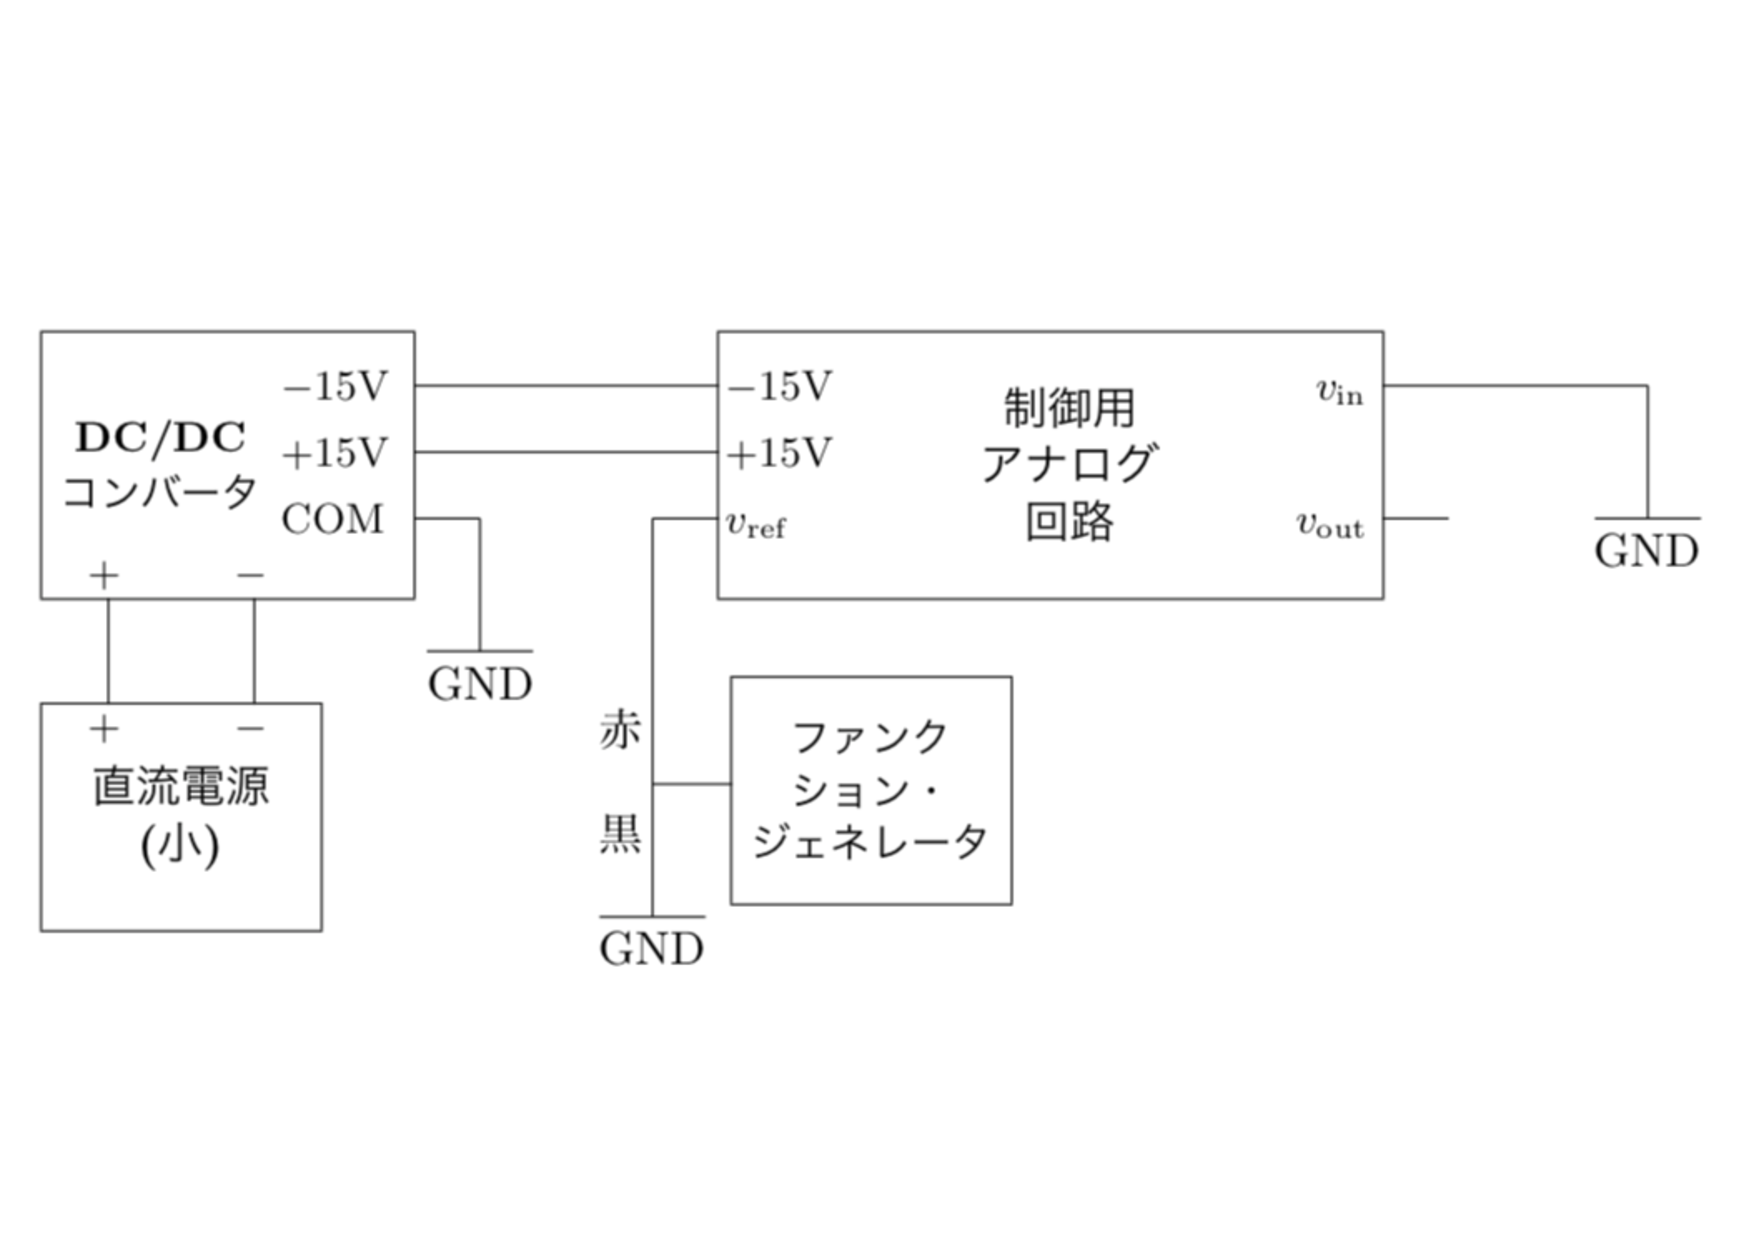
\includegraphics[width=12cm]{souchi2.pdf}
    \caption{実験2の測定装置}
    \label{souchi2}
\end{figure}

\newpage

\section{結果}

上で求めた理論値を用いて描いた理論グラフと測定によって得られた値を
プロットしたものをそれぞれ図\ref{idealplot3}、\ref{idealplot4}、
\ref{idealplot}、\ref{idealplot2}に示す。

ここで用いた測定値は、与えられたものである。

\begin{figure}[h]
    \centering
    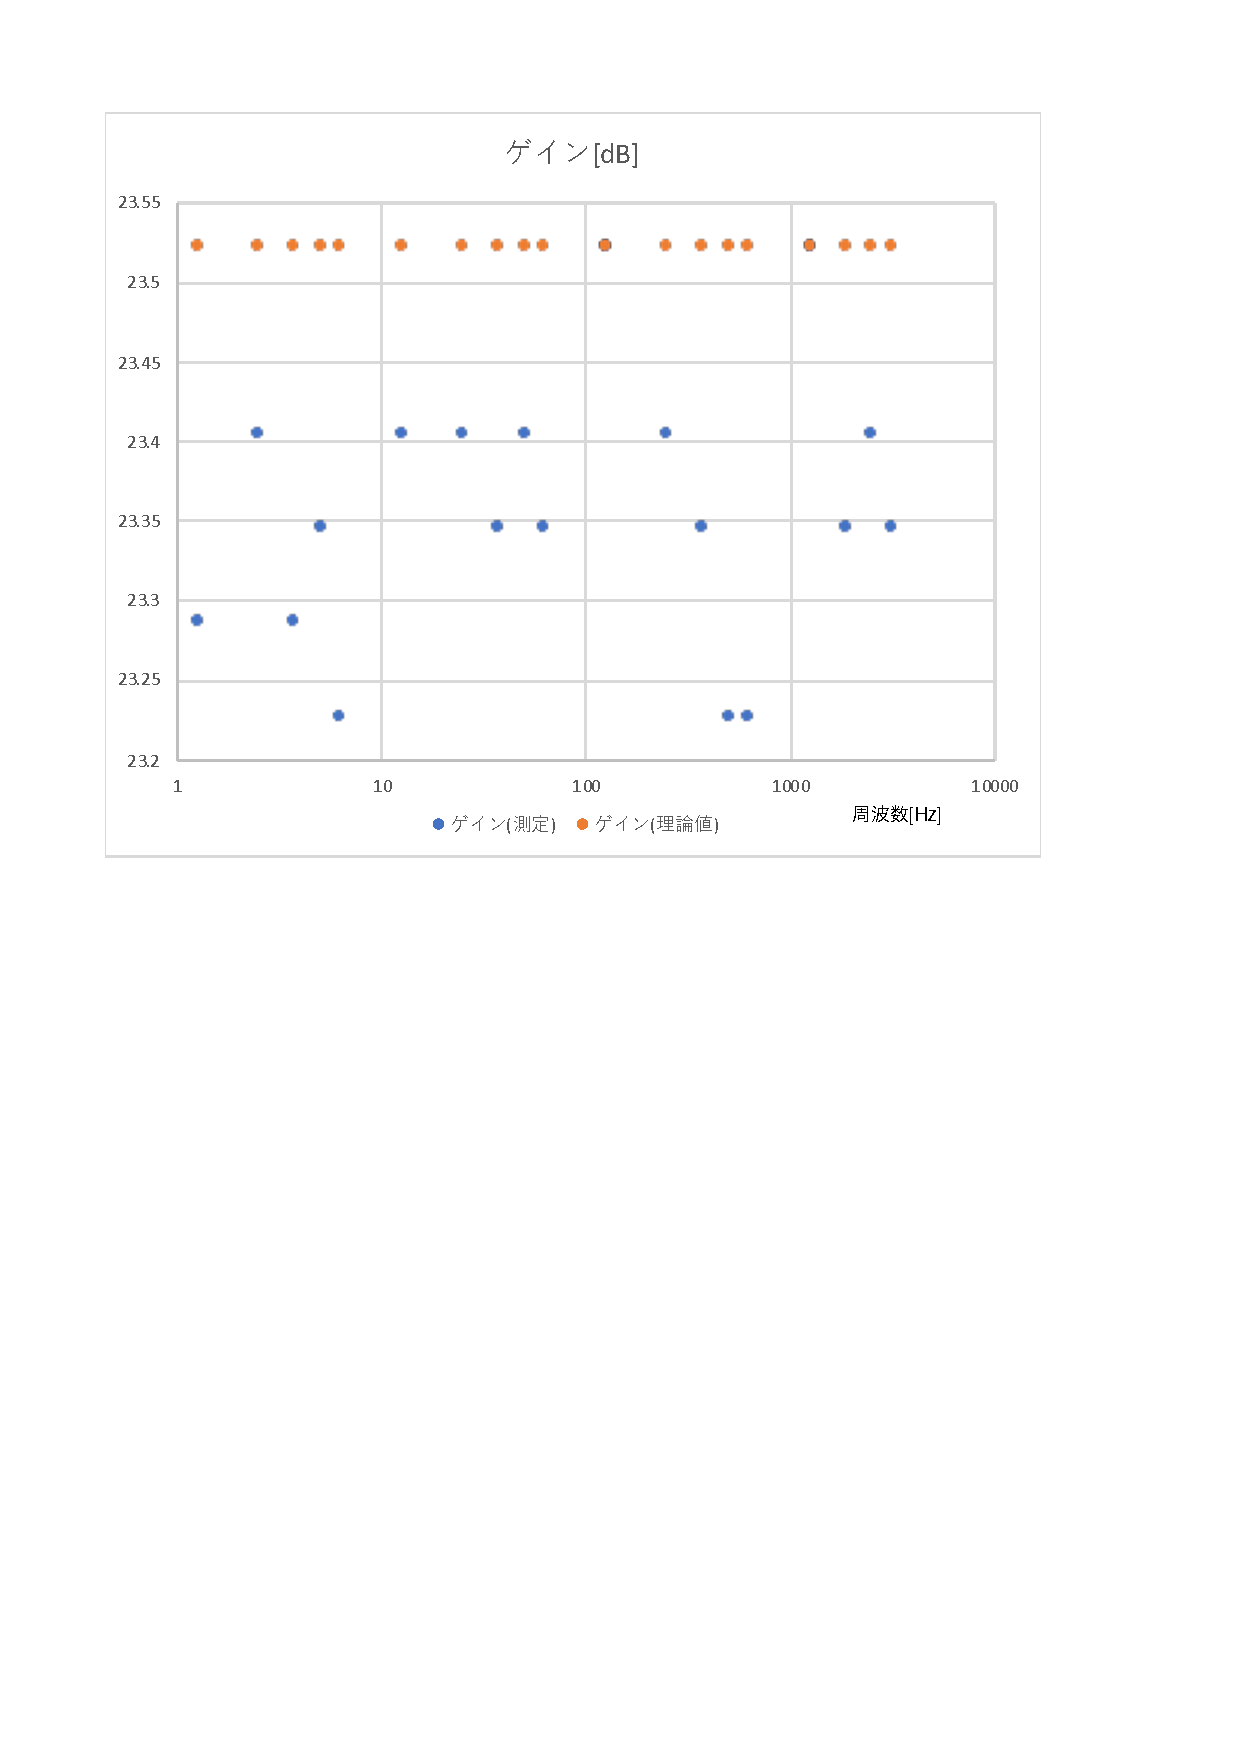
\includegraphics[width=9cm]{ideal_plot3.pdf}
    \caption{ゲイン(a)の測定値と理論値}
    \label{idealplot3}
\end{figure}

\begin{figure}[h]
    \centering
    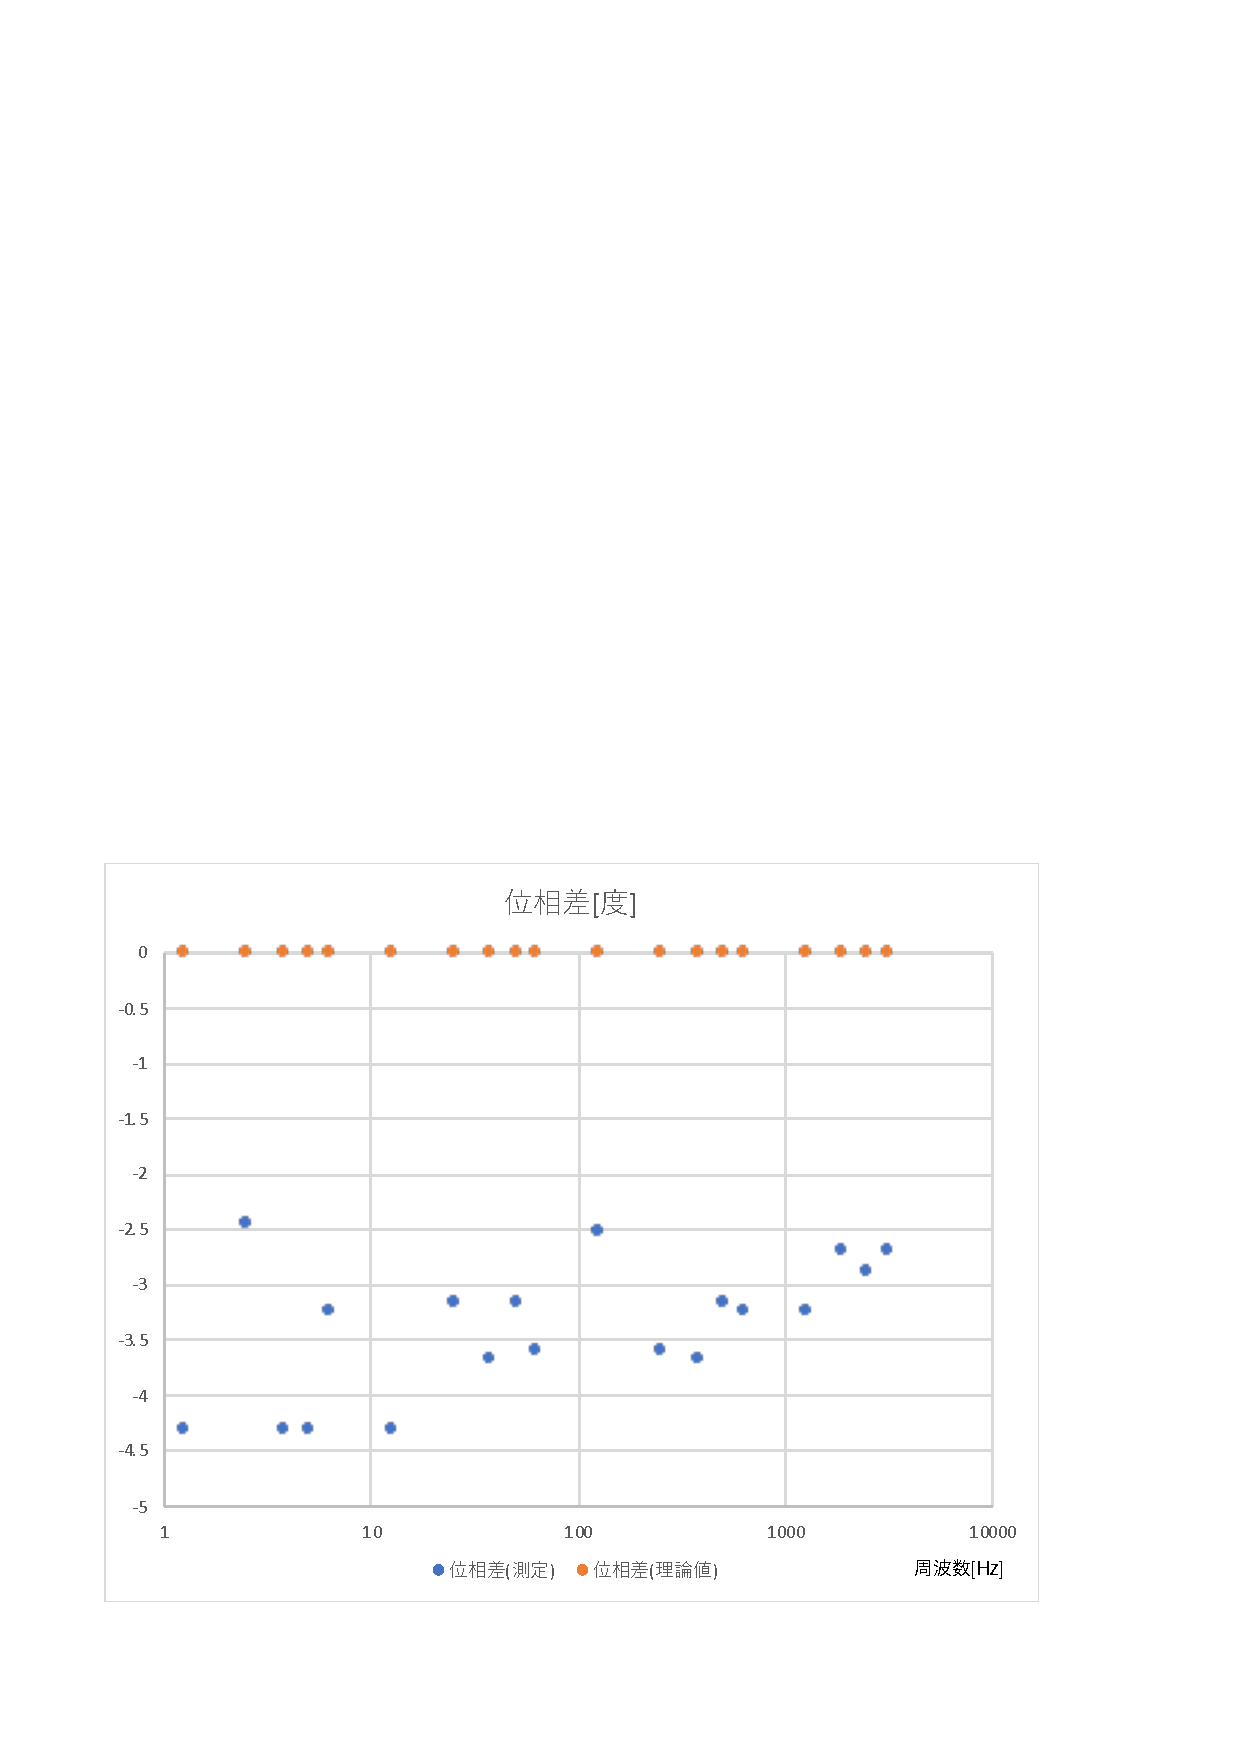
\includegraphics[width=9cm]{ideal_plot4.pdf}
    \caption{位相差(a)の測定値と理論値}
    \label{idealplot4}
\end{figure}

\begin{figure}[h]
    \centering
    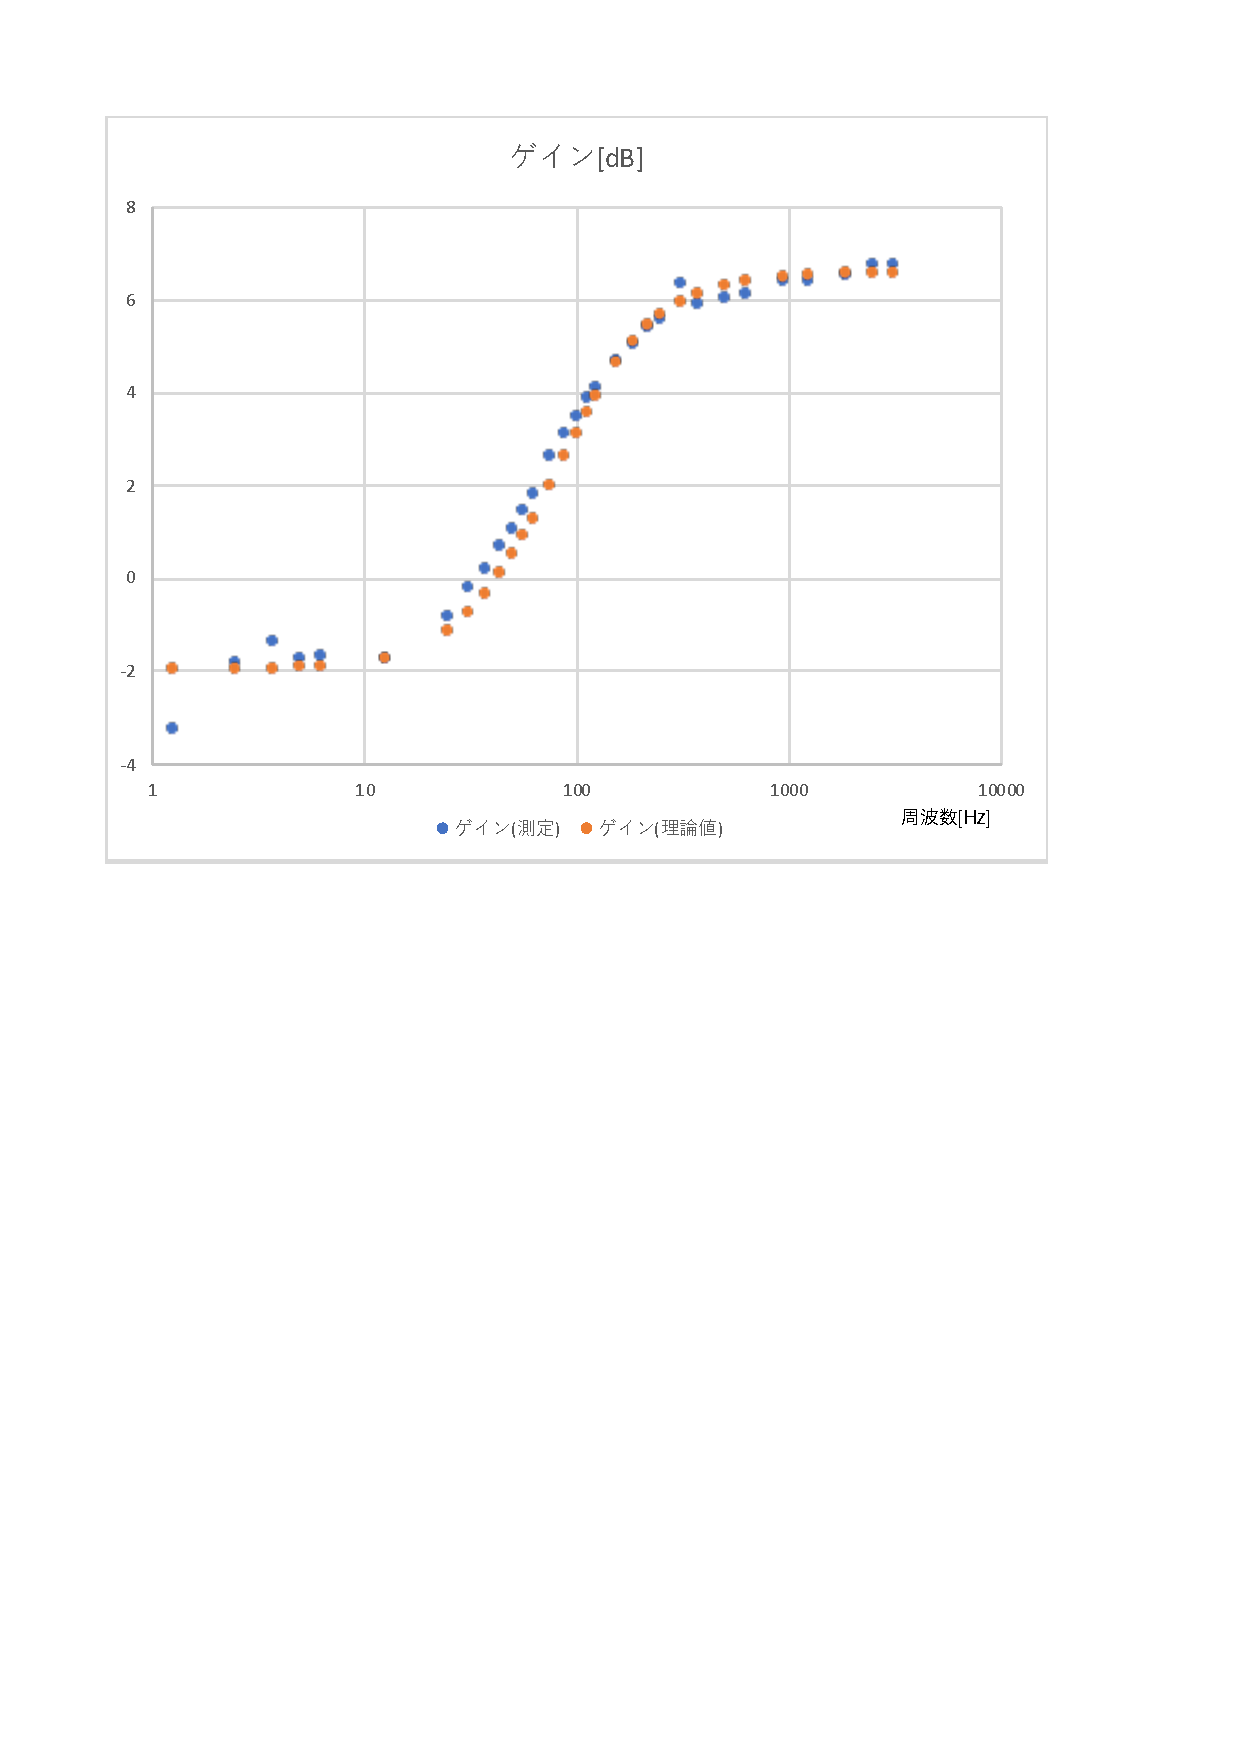
\includegraphics[width=9cm]{ideal_plot.pdf}
    \caption{ゲイン(b)の測定値と理論値}
    \label{idealplot}
\end{figure}

\begin{figure}[h]
    \centering
    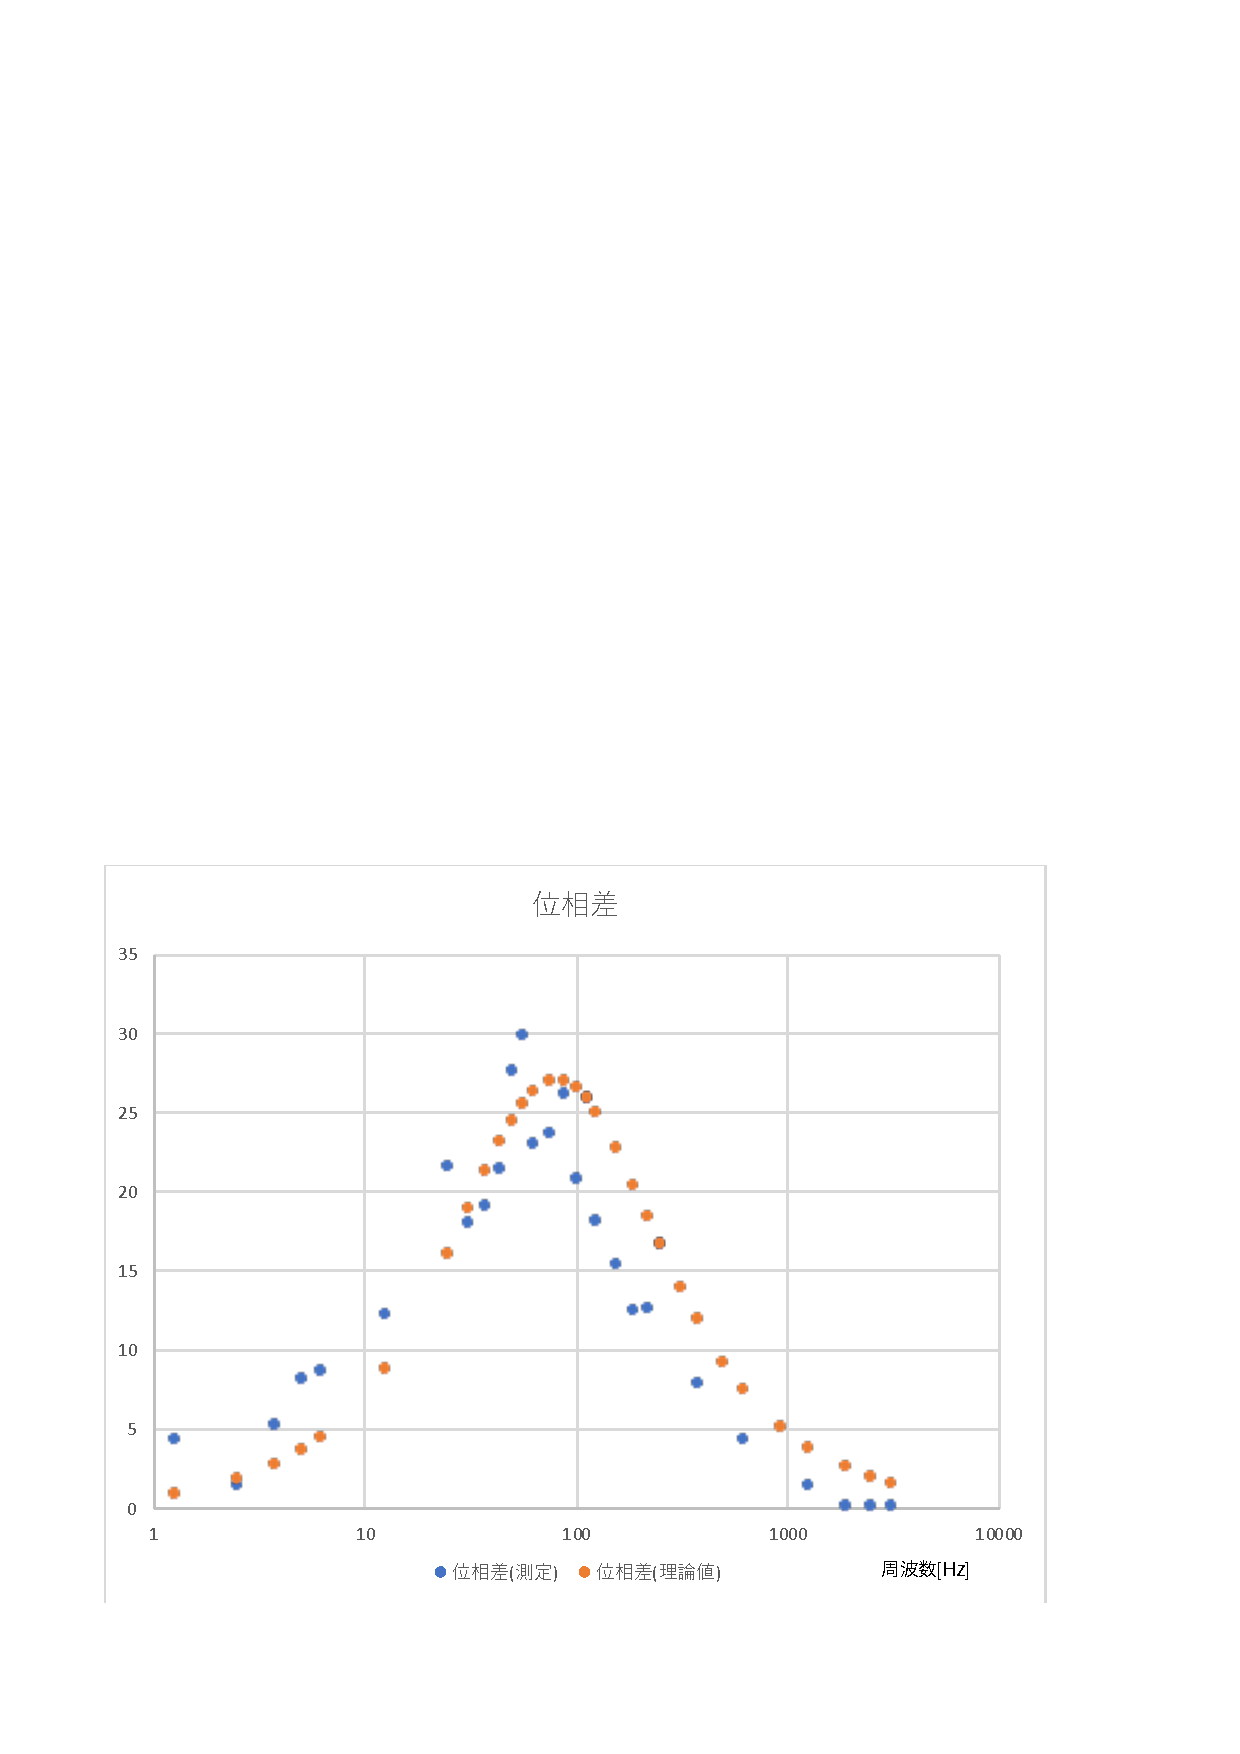
\includegraphics[width=9cm]{ideal_plot2.pdf}
    \caption{位相差(b)の測定値と理論値}
    \label{idealplot2}
\end{figure}


\newpage
\ 
\newpage
\ 
\newpage
\section{考察}

今回の測定値はオシロスコープから出力されたcsvファイルとして与えられた。
それを処理するためにRustで書いたプログラムを用いた。
そのコードをソースコード1に示す。

このコードでは、ふた通りの方法でゲインを求めたのち、
正弦波が0を示した点および0付近を示した点を列挙して、
実際のグラフと対比させながら位相差を求めた。
ゲインについて、まず全データの最大値、最小値を入力、出力それぞれについて
求め、比を求めた。しかし、この方法は最大値を示す一点のみから求めるので
ノイズに弱いと考えた。
二つ目の方法として、全データを絶対値をとって足し込んだのち、
測定間隔をかけ積分値とみなし、全データの観測時間をファイルの最初の
行と最後の行から求め振幅を計算してゲインを求めた。

この方法では低周波での観測において、位相差が0付近のデータを示すデータの数が
少ないと正しくデータが取れない可能性があるため目視で求めた測定データを
図\ref{mokushi1}、\ref{mokushi2}、\ref{mokushi3}、\ref{mokushi4}
に示すが、今回の計測ではむしろ位相差の高周波領域において上手く観測できていなかった
ことがわかった。これは、プログラムによる処理を高周波領域から始めたこと、
および観測するにつれて実際のデータに合わせてプログラムのパラメータを
調整したことによって生じた観測誤差だと考えた。

これらのグラフより、算出した各パラメータの値は正しいと結論づけた。

\begin{lstlisting}[caption={csv\_manager.rs}]
    use competitive::prelude::*;

#[argio()]
// csvファイルを読み取る
fn main(input: [(f32, f32, f32); 600]) {
    // 微小時間の幅を求める
    let dx = input[23].0.clone() - input[22].0.clone(); 
    // 配列の用意
    let mut v = Vec::new(); 
    let mut w = Vec::new();
    for i in 0..600 {
        // ch1, ch2のデータを一旦こちらにコピー
        v.push(input[i].1.clone()); 
        w.push(input[i].2.clone());
    }
    // 振幅の最大値を求める
    let max_ch1 = v.clone().into_iter().fold(0.0, f32::max); 
    let max_ch2 = w.clone().into_iter().fold(0.0, f32::max);
    println!("ch1'x max = {}", max_ch1);
    println!("ch2'x max = {}", max_ch2);

    // 全ての値を足しこむ変数を用意
    let mut sum1 = 0.0; 
    let mut sum2 = 0.0;
    for i in 0..600 {
        // 全て絶対値をとって足しこむ
        sum1 += v[i].clone().abs(); 
        sum2 += w[i].clone().abs();
    }
    //振幅を計算 
    let amp1 = dx * sum1 * 3.14 / 2.0 
        / (input[599].0.clone() - input[0].0.clone()); 
    let amp2 = dx * sum2 * 3.14 / 2.0 
        / (input[599].0.clone() - input[0].0.clone());
    println!("ch1::sum1: {}", amp1);
    println!("ch2::sum2: {}", amp2);

    // ゲインを出力
    println!("rate = {}", max_ch2 / max_ch1); 
    println!("rate2 = {}", sum2 / sum1);

    println!("");
    println!("");

    // こっから下で-3e-2~3e-2の間に入る点をピックアップ
    // 特に丁度0になった点はメッセージを短くして目立つようにした
    for i in 0..600 {
        if input[i].1 == 0.0 {
            println!("ch1 = 0: {}, {}", 
                input[i].0.clone(), input[i].1.clone());
        } else if input[i].1 >= -3.00e-2 
               && input[i].1 <= 3.00e-2 
        {
            println!(
                "maybe ch1 = 0: {}, {}",
                input[i].0.clone(),
                input[i].1.clone()
            );
        }
        if input[i].2 == 0.0 {
            println!("ch2 = 0: {}, {}", 
                input[i].0.clone(), input[i].2.clone());
        } else if input[i].2 >= -3.00e-2 
               && input[i].2 <= 3.00e-2 
        {
            println!(
                "maybe ch2 = 0: {}, {}",
                input[i].0.clone(),
                input[i].2.clone()
            );
        }
    }
}
\end{lstlisting}

\begin{figure}[h]
    \centering
    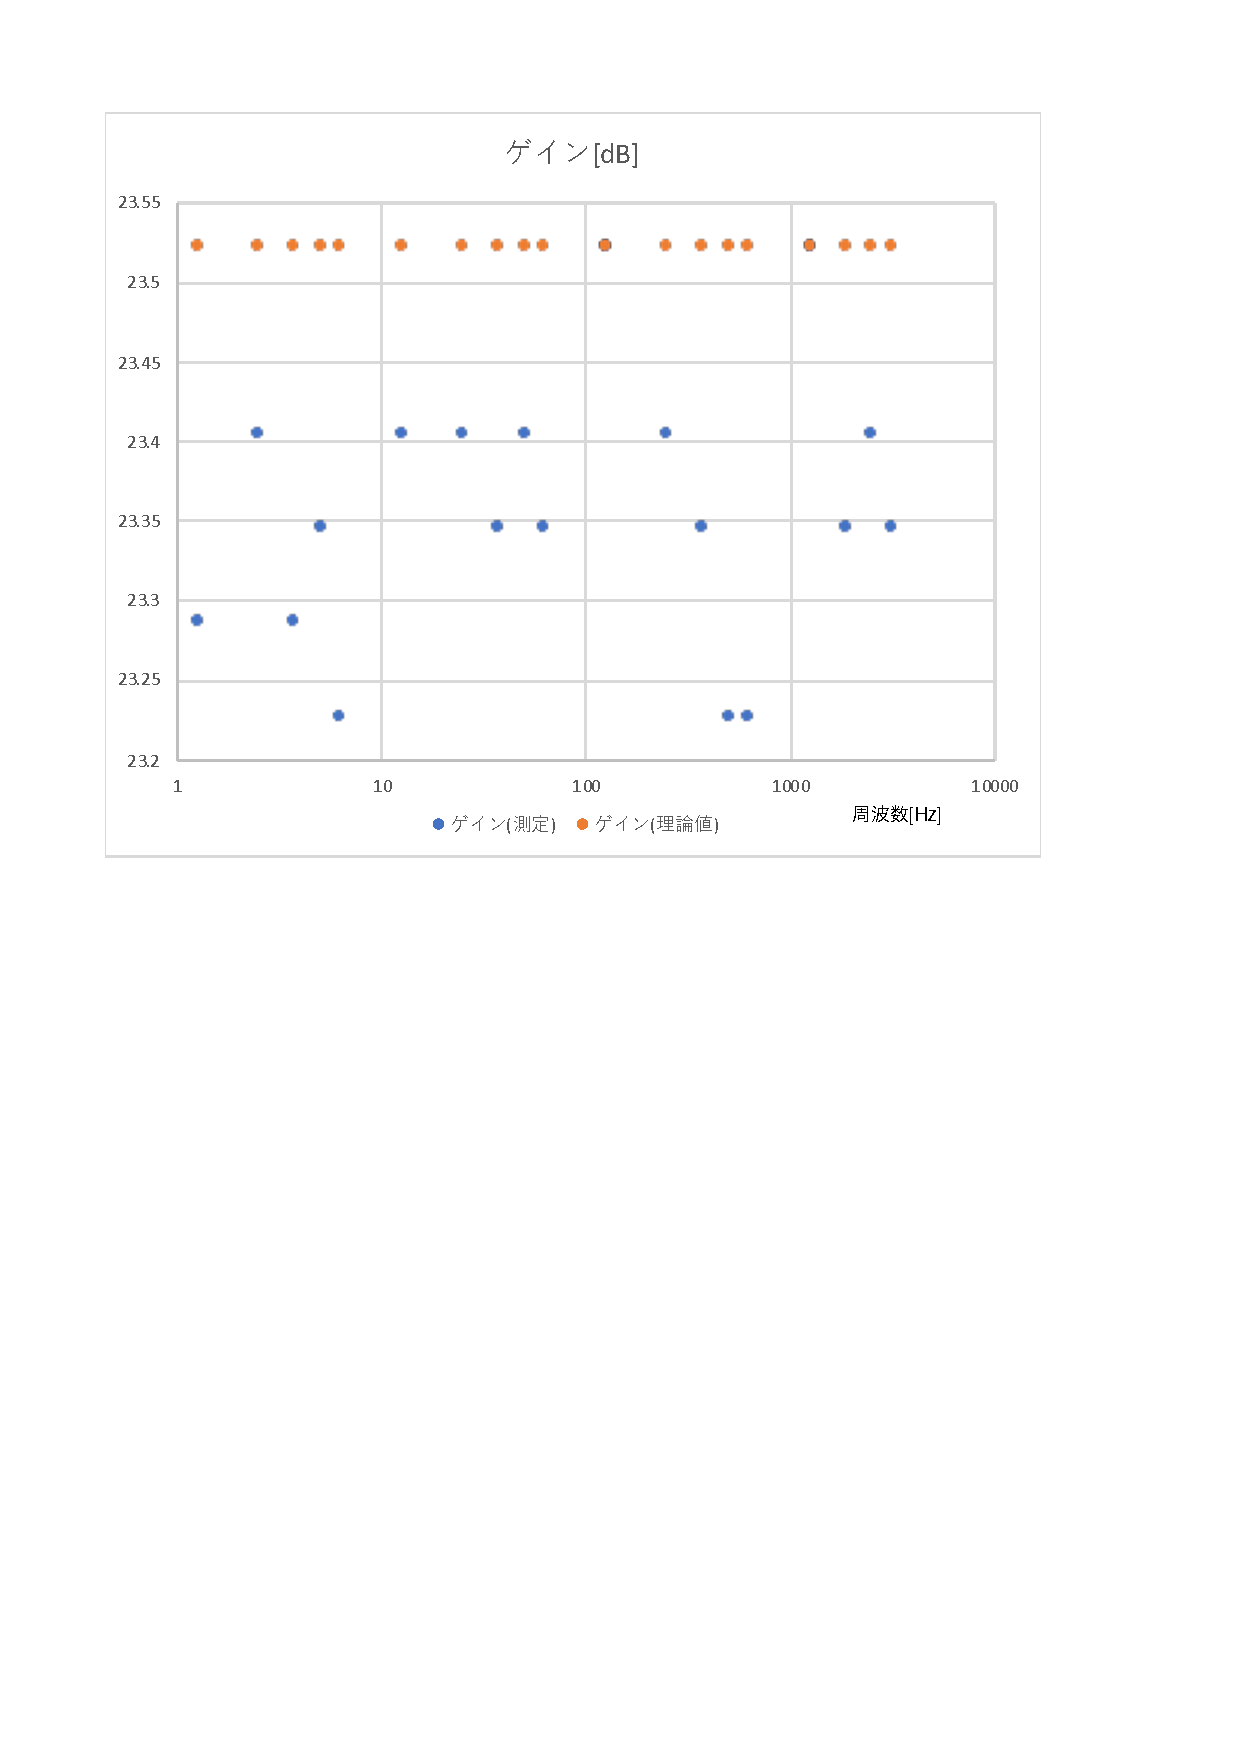
\includegraphics[width=9cm]{mokushi1.pdf}
    \caption{ゲイン(a)の測定値と理論値(目視)}
    \label{mokushi1}
\end{figure}

\begin{figure}[h]
    \centering
    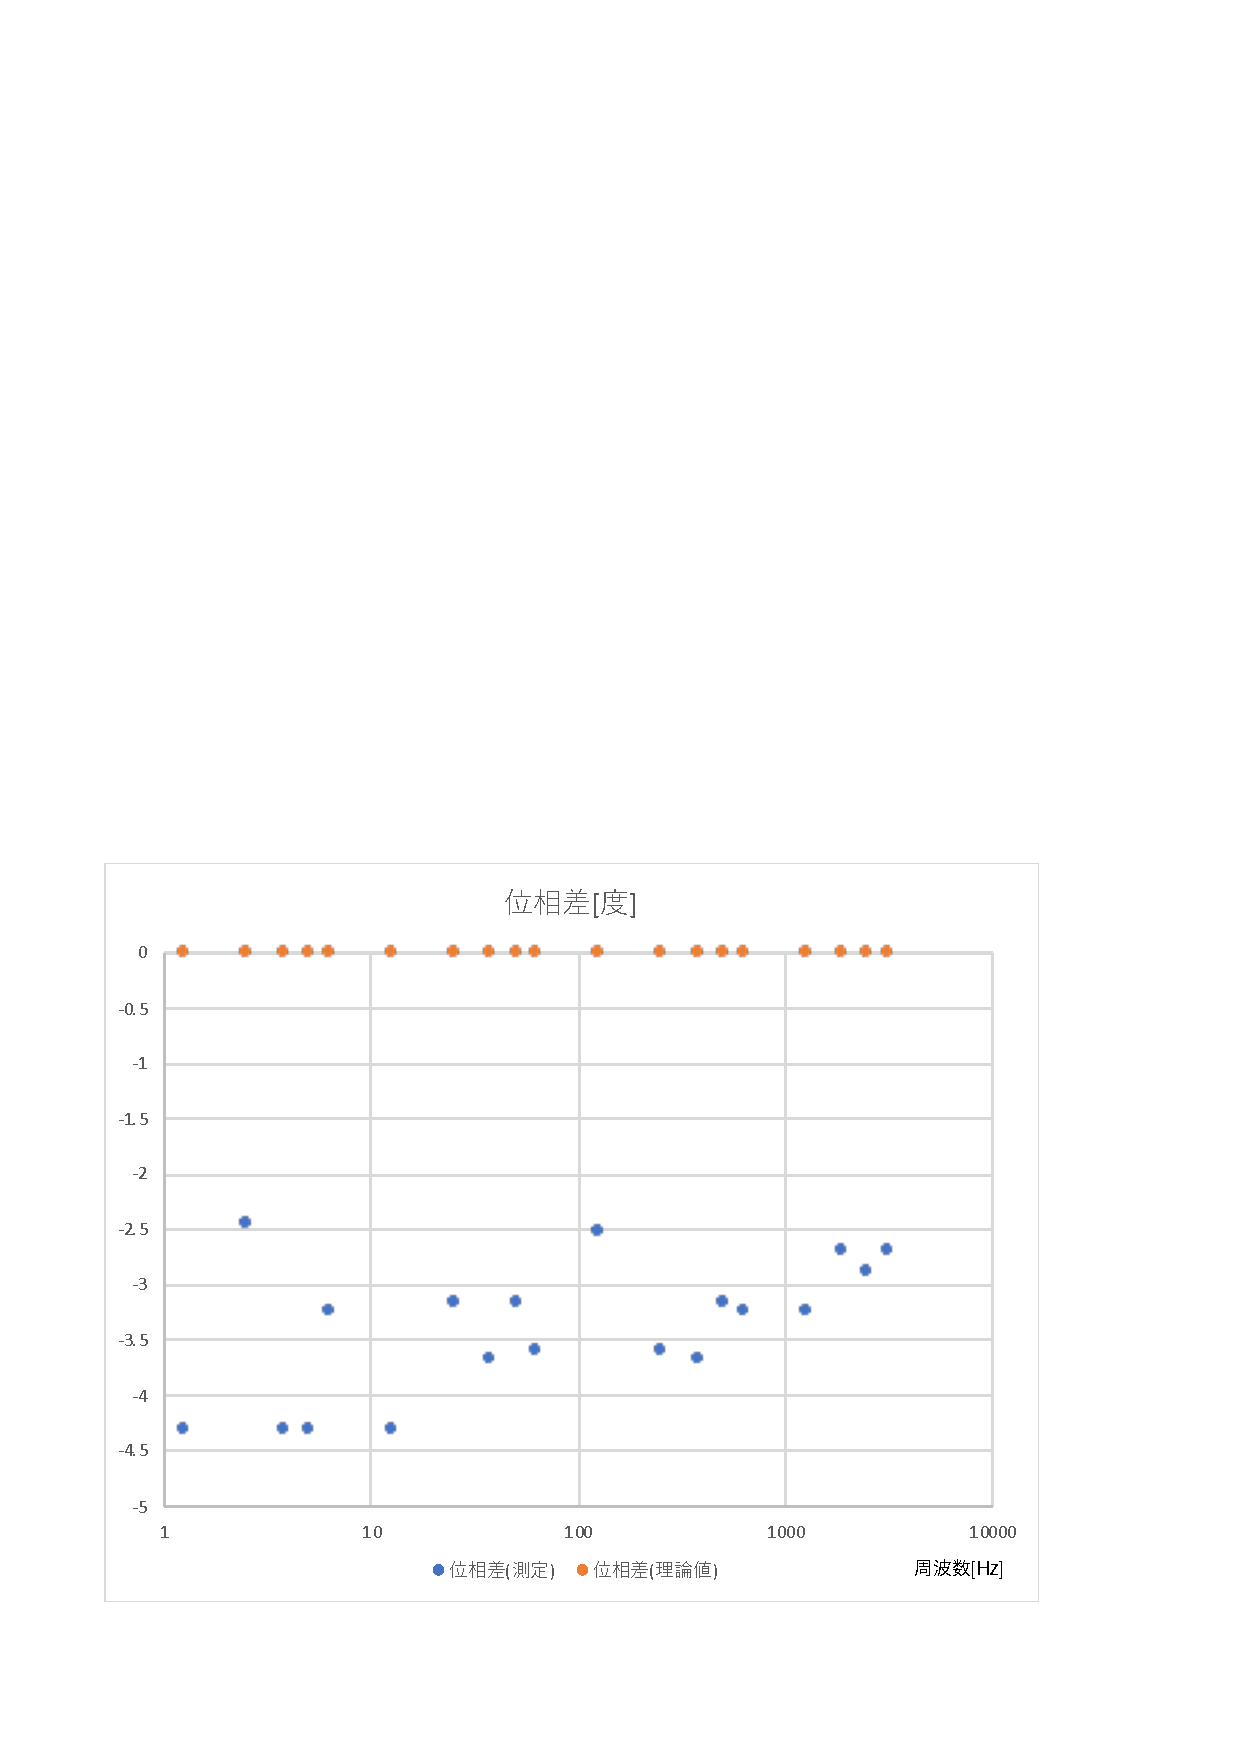
\includegraphics[width=9cm]{mokushi2.pdf}
    \caption{位相差(a)の測定値と理論値(目視)}
    \label{mokushi2}
\end{figure}

\begin{figure}[h]
    \centering
    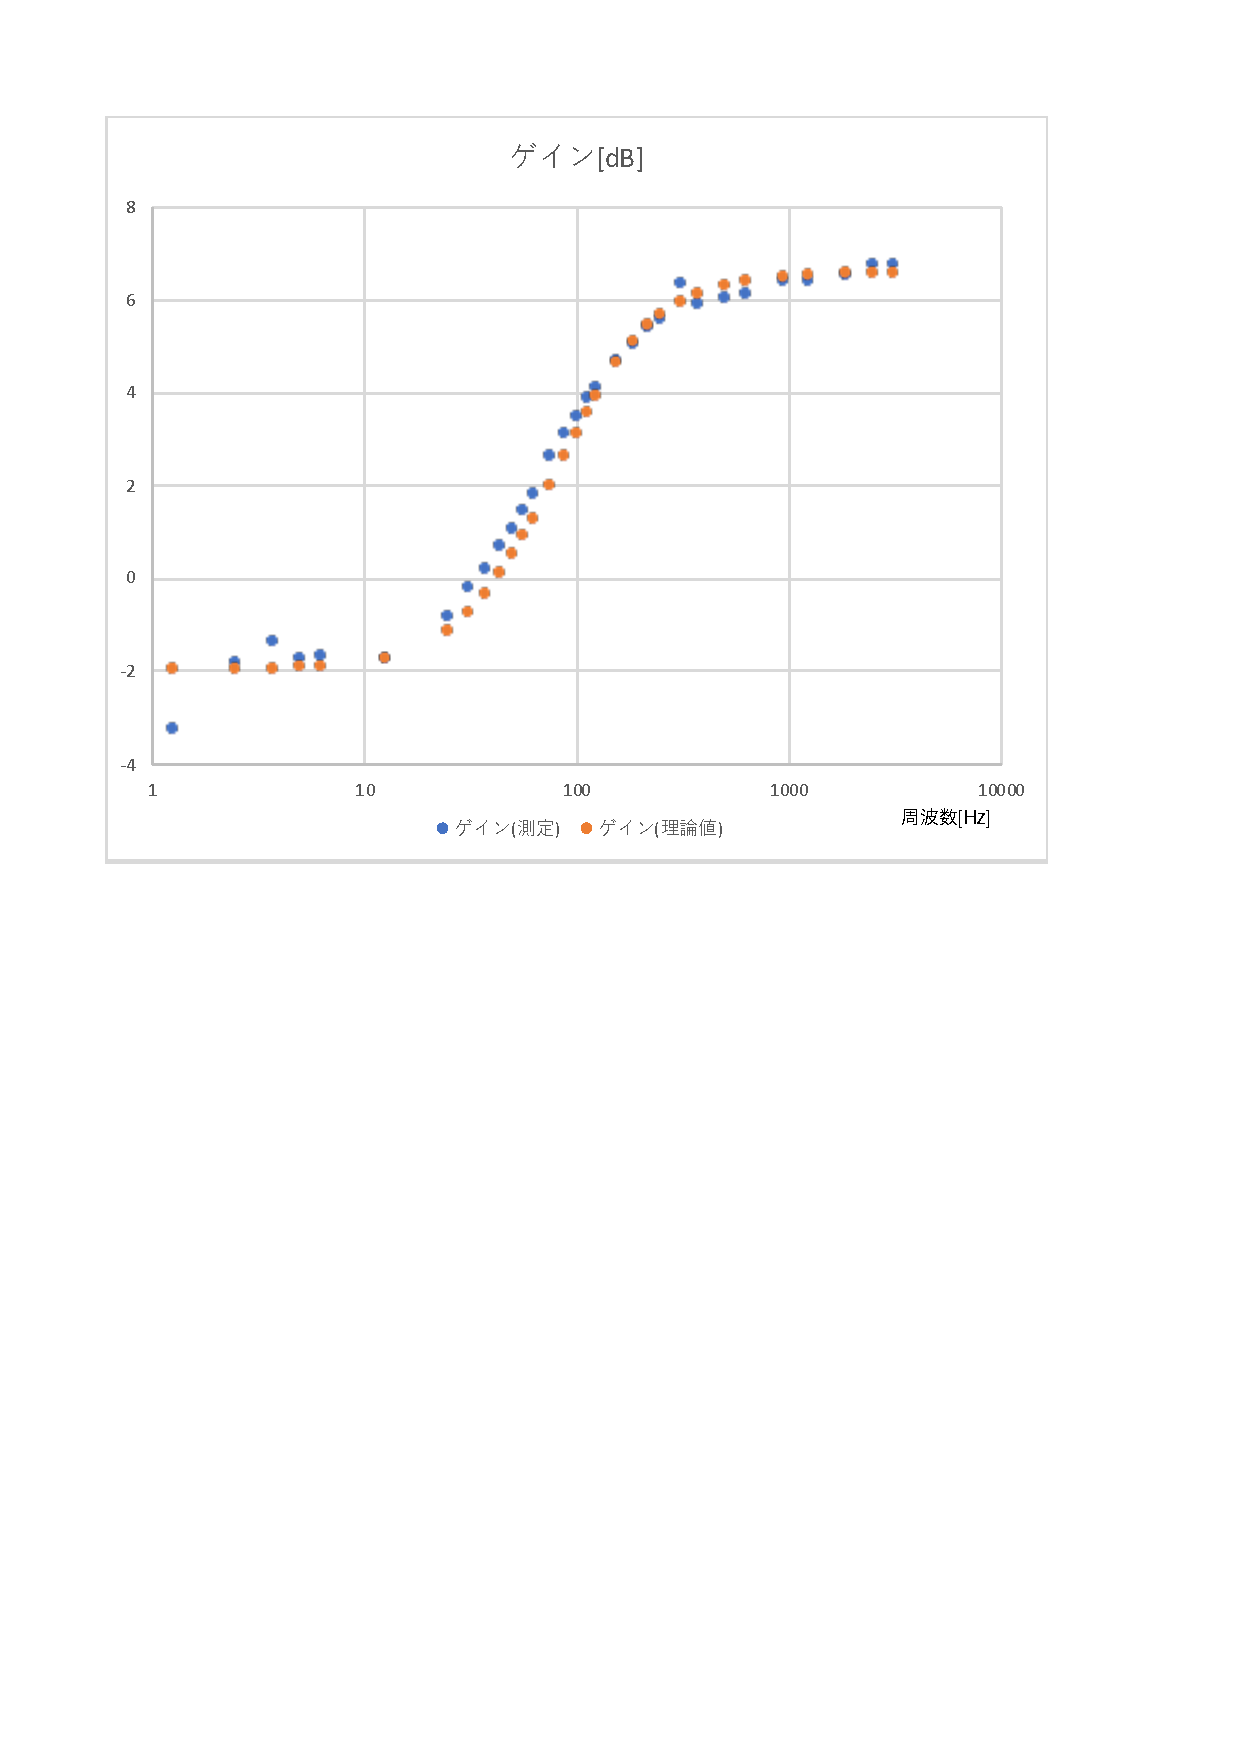
\includegraphics[width=9cm]{mokushi3.pdf}
    \caption{ゲイン(b)の測定値と理論値(目視)}
    \label{mokushi3}
\end{figure}

\begin{figure}[h]
    \centering
    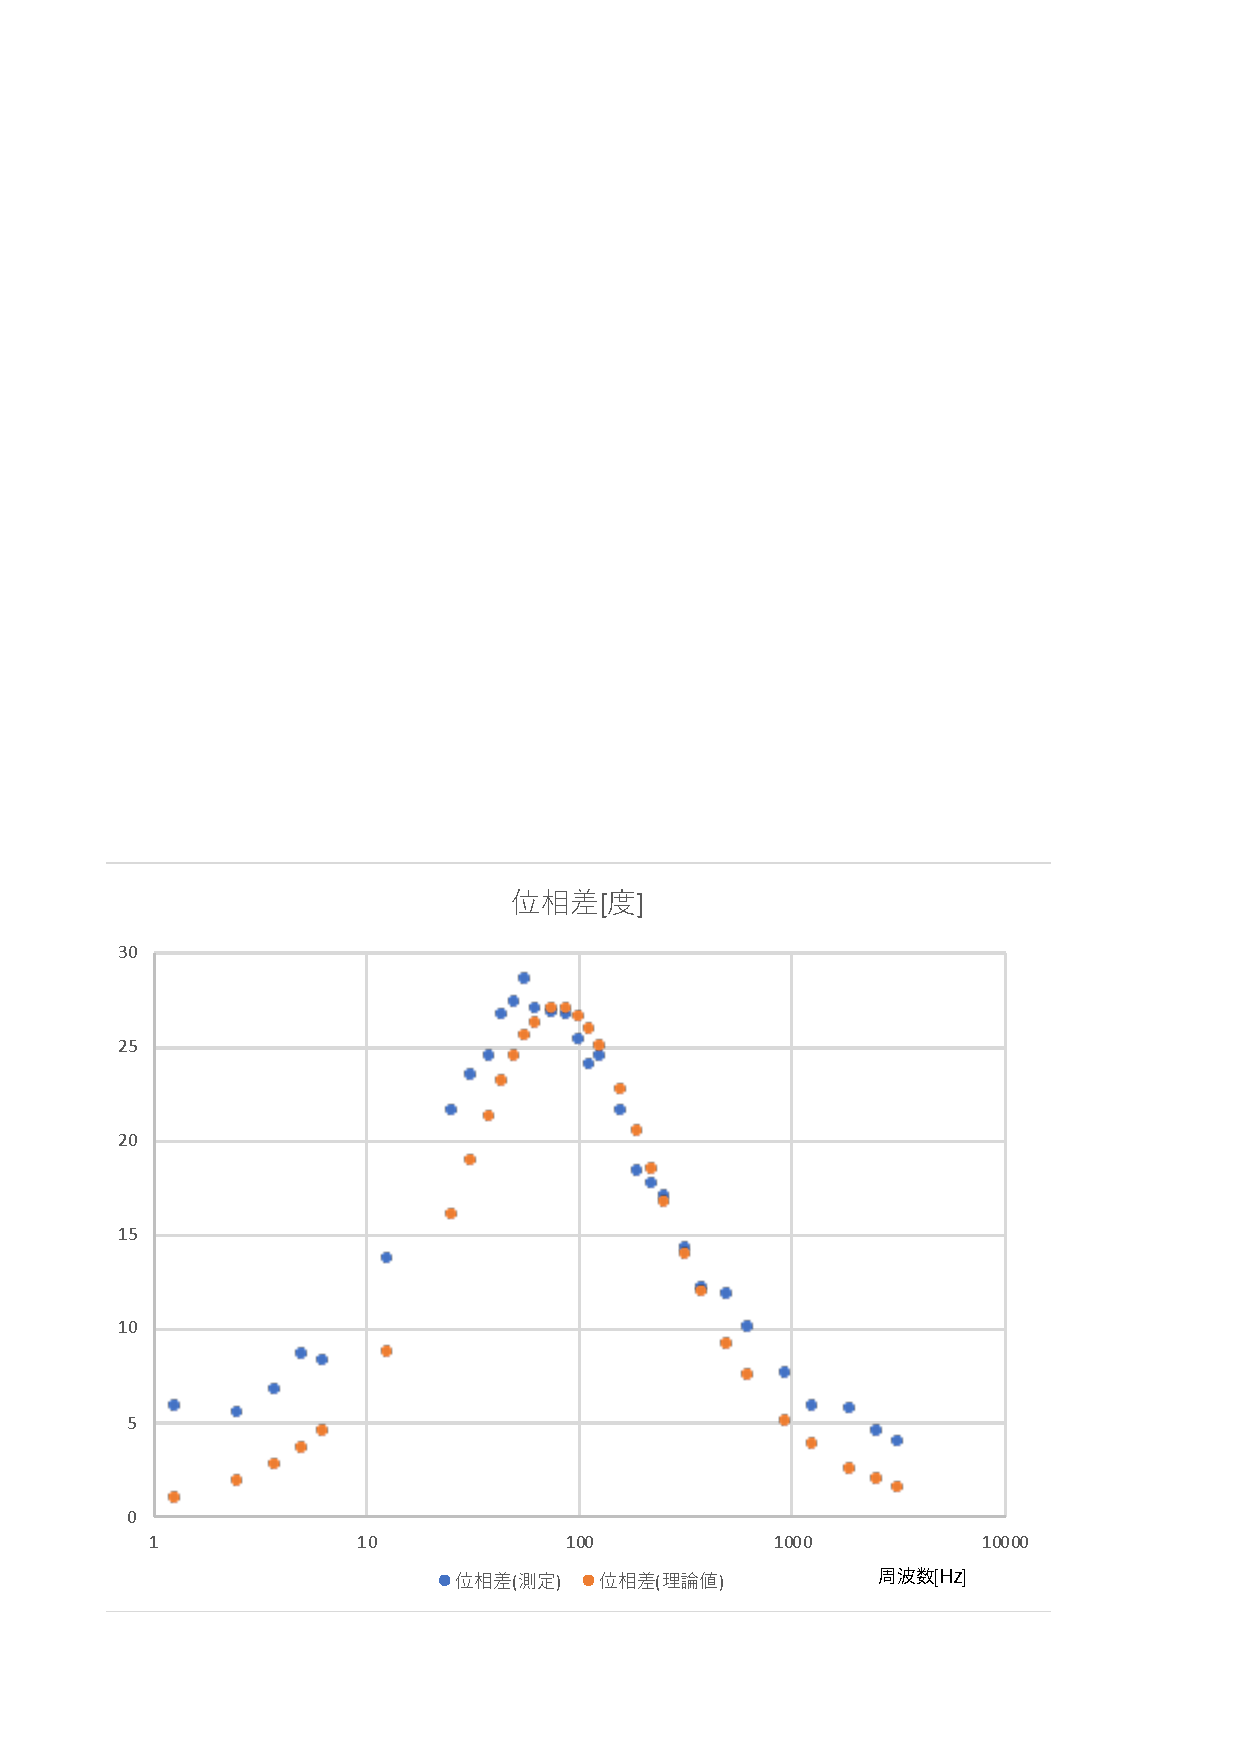
\includegraphics[width=9cm]{mokushi4.pdf}
    \caption{位相差(b)の測定値と理論値(目視)}
    \label{mokushi4}
\end{figure}

% 実験レポート2
% ここまで

\newpage


% 実験レポート3
% ここから

% \subtitle{2020/11/6}

\newpage
\ 
\newpage

\theme{実験3}

\section{目的}
実験2で作成したアナログ制御回路を用いて
DCサーボモータの速度制御、位置制御をそれぞれ行い、
安定性と定常偏差について調べる。
また実験結果とOctaveを用いたシミュレーションを比較する。

\section{原理}

今実験で用いた回路のボード線図は、図\ref{gaizu}のようなブロック線図で
表現できる。

したがって、制御系の安定性を調べるには

\begin{equation}\label{antei}
    \frac{C(s)P(s)}{1+C(s)P(s)}
\end{equation}

についてラウスやナイキストの安定判別を行えば良い。
また、定常偏差の伝達関数は

\begin{equation}\label{hensa}
    \frac{1}{1+C(s)P(s)}
\end{equation}

として得られる。

\begin{figure}[h]
    \centering
    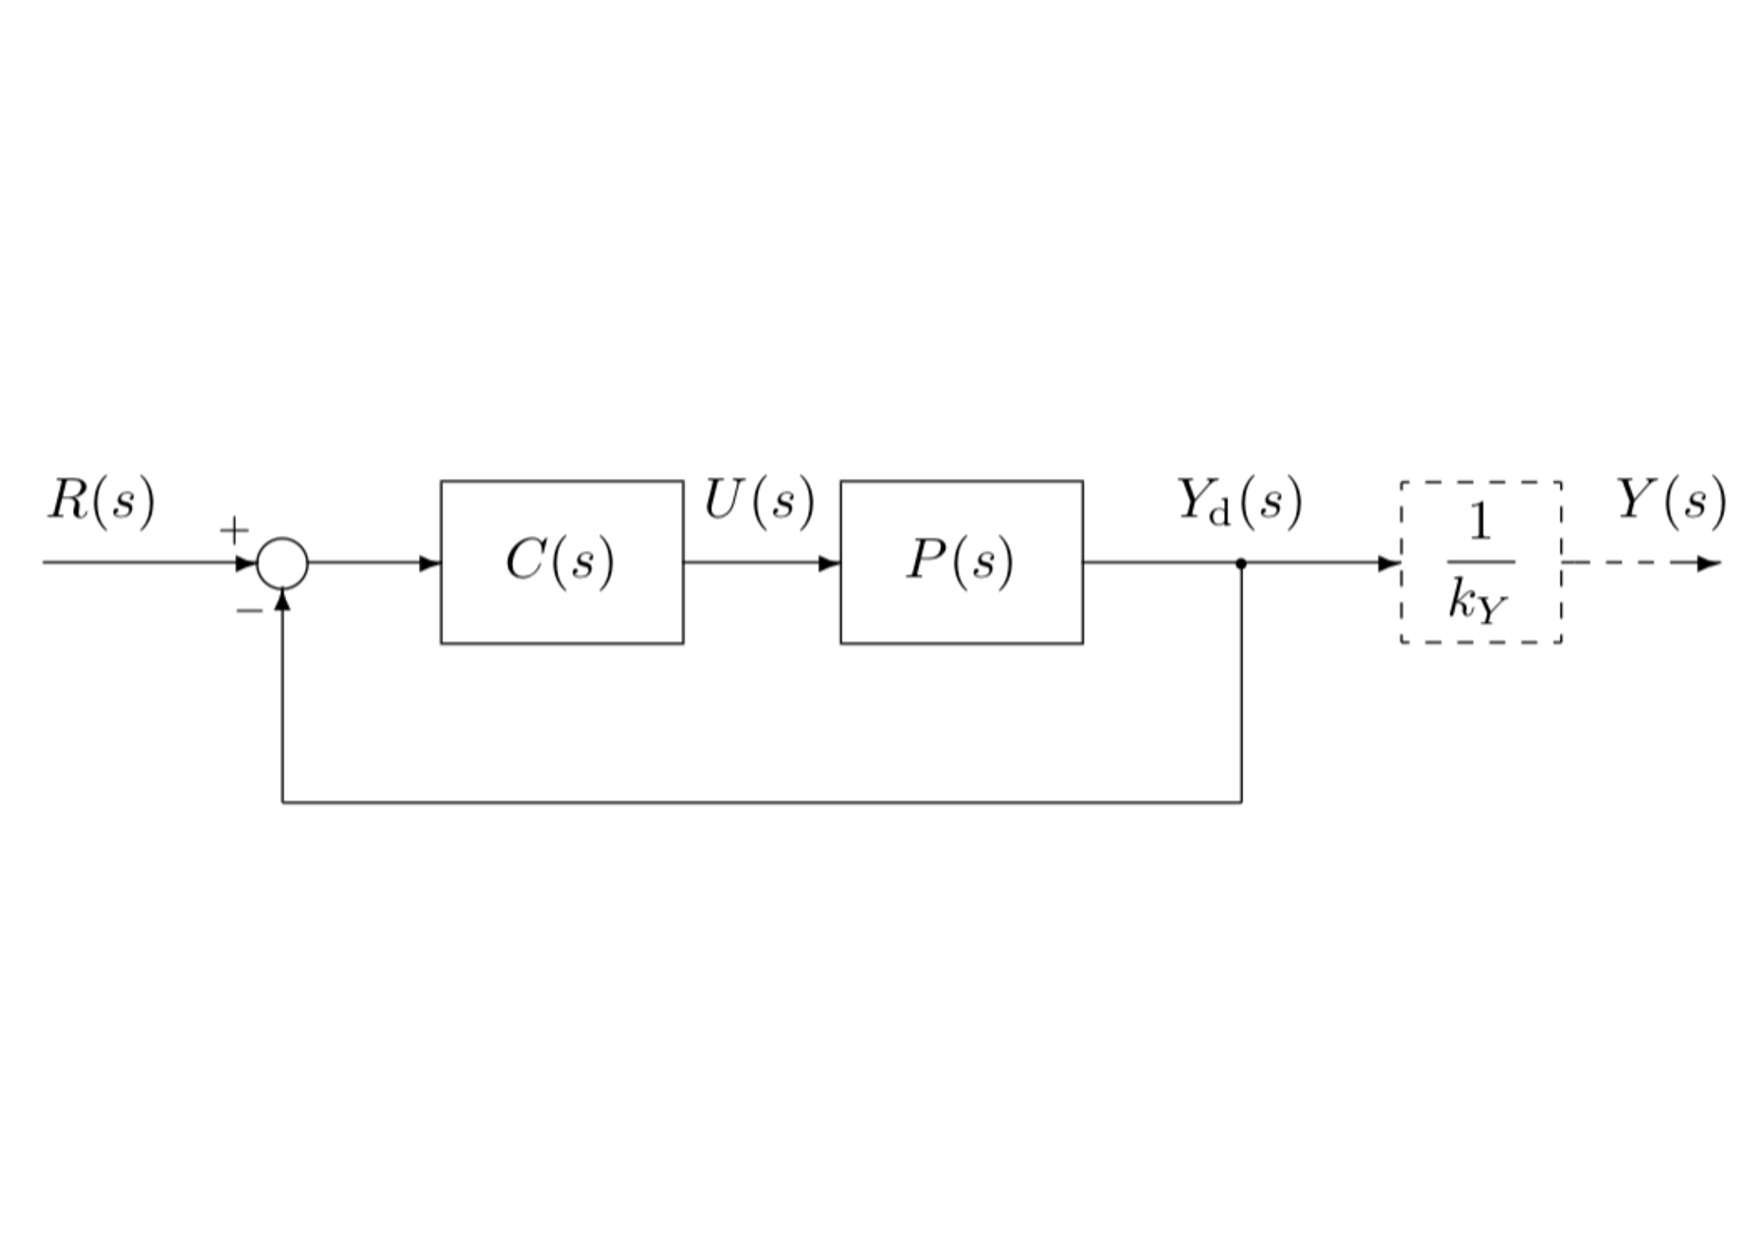
\includegraphics[width=12cm]{gaizu.pdf}
    \caption{ブロック線図(概略図)}
    \label{gaizu}
\end{figure}


\section{実験}

アナログ制御回路には、実験2で作成したものを用いた。
このアナログ制御回路を用いてDCサーボモータの速度制御および
位置制御を行う。安定性を先に判別し、安定な組み合わせに関してのみ
ステップ応答を測定した。

また、Octaveを用いて理論的なグラフを描き、
実験結果を重ねてステップ応答を比較した。

\section{結果}

まず(a)、(b)の制御回路を用いて速度制御、位置制御をした時の安定性を
ラウスの安定判別法を用いて判別した。
そして安定な制御系は最終値公式を用いて定常偏差を計算した。

ラウスの安定判別法は、式\ref{antei}の分母A(s)について行う。

まず(a)の制御回路を用いて速度制御した場合の分母は、

\begin{equation}
    A_1(s) = 1.117\times10^{-4}s^2 + 9.13\times10^{-2} s + 16.5
\end{equation}

となる。この式は2次式であり、係数が全て正なのでこの制御は安定であると考えた。
この制御系のステップ応答の定常偏差を最終値公式を用いて求めると

\begin{equation}
    \lim_{s \to 0} \frac{1}{1 + C(s)P(s)} = 
        \lim_{s \to 0} \frac{1}{1.17\times10^{-4}s^2 + 9.13\times10^{-2}s + 16.45}
            = 0.061
\end{equation}

次に(a)の制御回路を用いて位置制御した場合の分母は

\begin{equation}
    A_2(s) = 3.35\times10^{-6}s^3 + 2.61\times10^{-3}s^2 
        + 2.86\times10^{-2}s + 73.7
\end{equation}

となる。これに対しラウスの安定判別を行うと

\begin{table}[h]
    \centering
    \begin{tabular}{|c||c|c|} \hline
        行 & 1 & 2 \\ \hline \hline
        1 & $3.35\times10^{-6}$ & $2.86\times10^{-2}$ \\ \hline
        2 & $2.61\times10^{-3}$ & 73.65 \\ \hline
        3 & $-6.59\times10^{-2}$ & \  \\ \hline
        4 & 73.65 & \  \\ \hline
    \end{tabular}
\end{table}

となる。ここで3行1列目で負の数が現れるので、この制御系は
不安定であると考えた。

次に、(b)の制御回路を用いて速度制御する場合を考えると

\begin{equation}
    A_3(s) = 8.78\times10^{-7}s^3 + 8.02\times10^{-4}s^2 
        + 1.15\times10^{-1}s + 1.82
\end{equation}

となる。これに対しラウスの安定判別法を用いると

\begin{table}[h]
    \centering
    \begin{tabular}{|c||c|c|} \hline
        行 & 1 & 2 \\ \hline \hline
        1 & $8.78\times10^{-7}$ & $1.15\times10^{-1}$ \\ \hline
        2 & $8.02\times10^{-4}$ & 1.82 \\ \hline
        3 & $1.13\times10^{-1}$ & \  \\ \hline
        4 & 1.82 & \  \\ \hline
    \end{tabular}
\end{table}

したがってこの制御系は安定であると考えた。
この制御系の定常偏差を求めると

\begin{equation}
    \lim_{s \to 0}\frac{1}{1+C(s)P(s)} 
        = \frac{1\times1.03}{1.82} = 0.57 
\end{equation}

最後に(b)の制御回路を用いて位置制御する場合を考えると

\begin{equation}
    A_4(s) = 2.51\times10^{-8} s^4 + 2.29\times10^{-5}s^3 
        + 2.82\times10^{-3}s^2 
        + 1.07\times10^{-1}s + 3.92
\end{equation}

となる。これに対しラウスの安定判別法を用いると

\begin{table}[h]
    \centering
    \begin{tabular}{|c||c|c|c|} \hline
        行 & 1 & 2 & 3 \\ \hline \hline
        1 & $2.51\times10^{-8}$ & $2.82\times10^{-3}$ & 3.92 \\ \hline
        2 & $2.29\times10^{-5}$ & 0.107 & \  \\ \hline
        3 & $2.70\times10^{-3}$ & 3.92 & \  \\ \hline
        4 & 1.82 & \ & \  \\ \hline
        5 & 3.92 & \ & \ \\ \hline
    \end{tabular}
\end{table}

となる。したがって、この制御系も安定であると考えた。
この制御系の定常偏差は

\begin{equation}
    \lim_{s \to 0} \frac{1}{1 + C(s)P(s)} 
        = \frac{0}{3.91} = 0
\end{equation}

と求まる。

以上の結果は、実験時に実際に制御させ安定かどうかを
現象として判定した結果と合致する。

以上の結果を元に、制御回路(a)での速度制御および制御回路(b)での位置制御を
行い、実測値と計算結果を比較したグラフを図\ref{07in}、\ref{08in}、
\ref{09in}に示す。制御回路(b)による制御は理論値に近い結果が得られたが、
制御回路(a)よる制御は期待通りの結果にならなかった。

またステップ応答の結果と理論値をOctaveを用いて
重ねたものをそれぞれ図\ref{unitvain}、\ref{unitvaout}、
\ref{unitvbin}、\ref{unitvbout}、\ref{unitpbin}、\ref{unitpbout}
に示す。なお、制御回路(a)による速度制御の$v_{\rm out}$はオシロスコープから
データを取り出す段階でデータが壊れてしまい、描画できなかった。
そのため計算結果に基づくシミュレーションのみを描画した。

\begin{figure}[h]
    \centering
    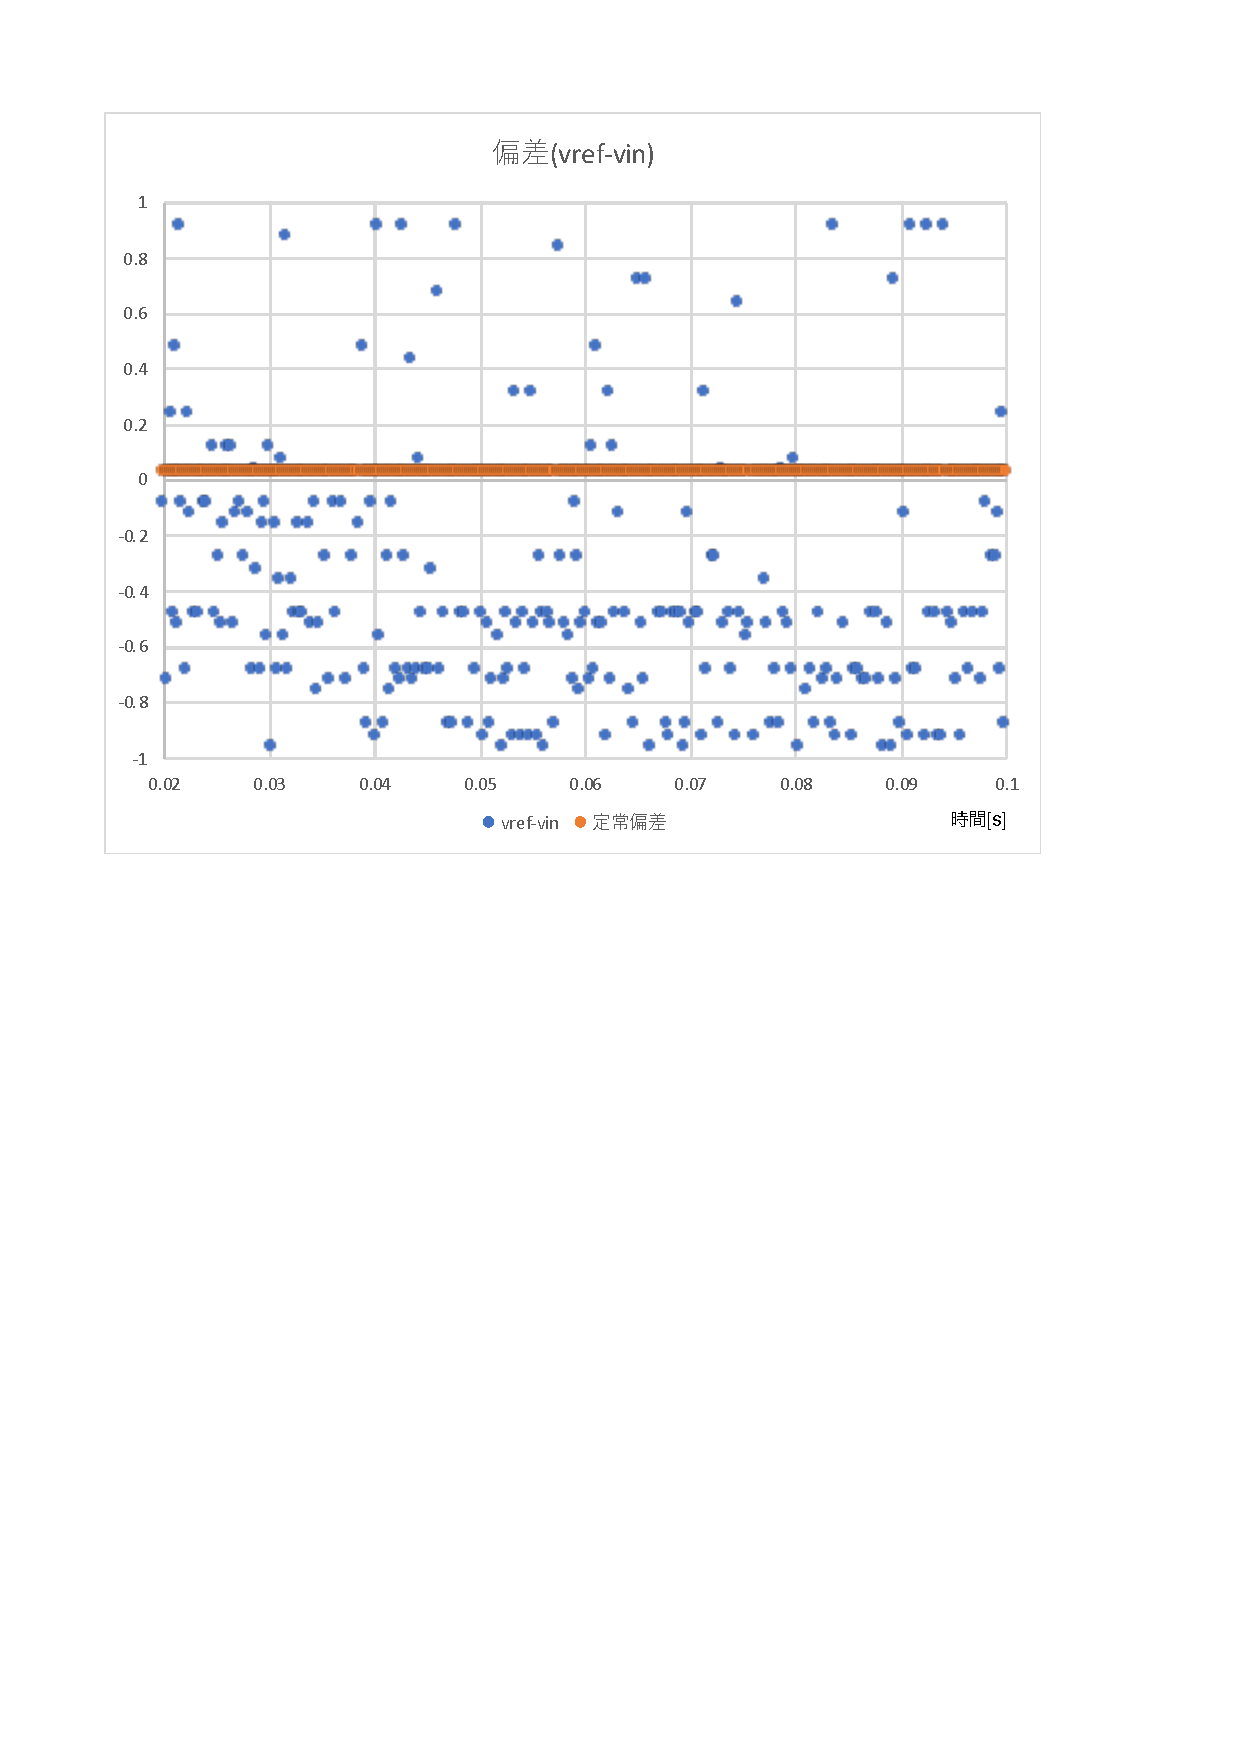
\includegraphics[width=9cm]{07in.pdf}
    \caption{制御回路(a)の速度制御}
    \label{07in}
\end{figure}

\begin{figure}[h]
    \centering
    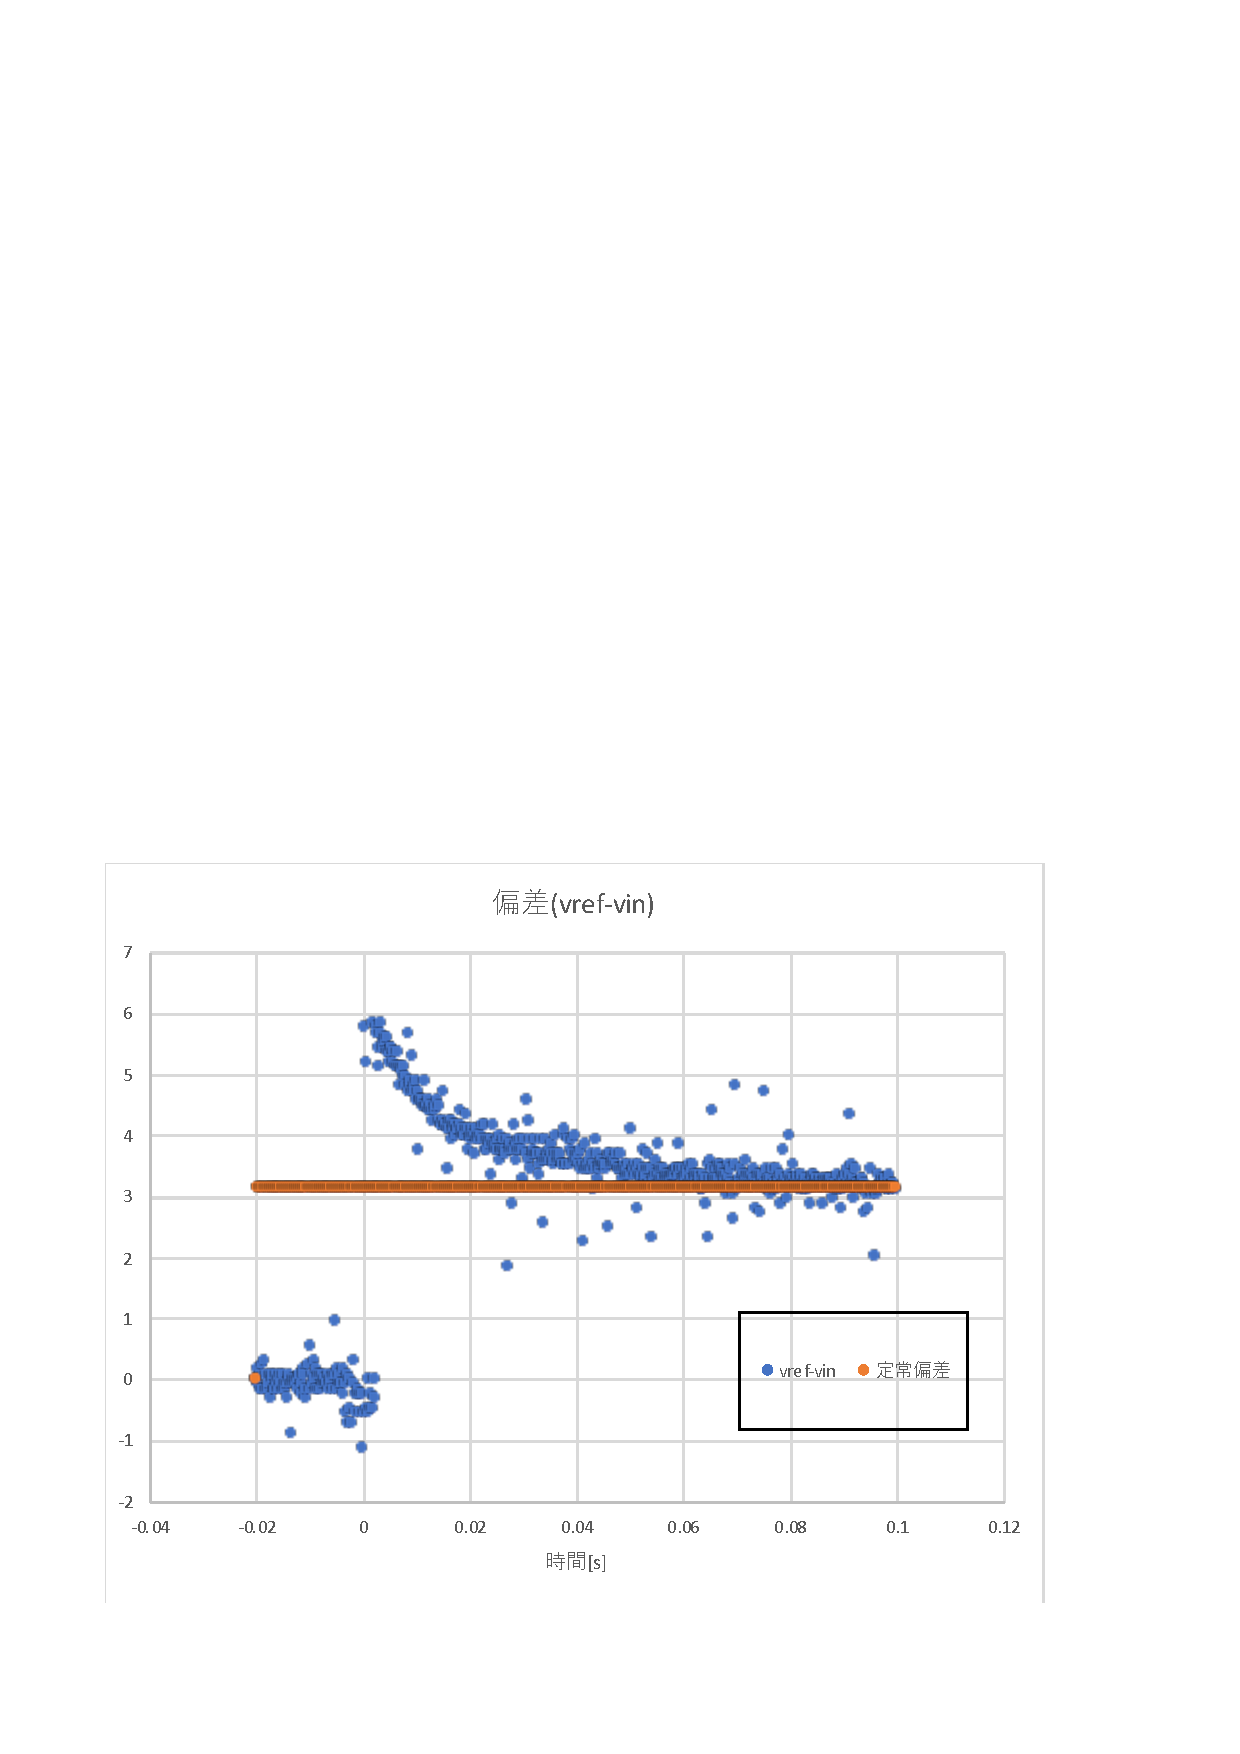
\includegraphics[width=9cm]{08in.pdf}
    \caption{制御回路(b)の速度制御}
    \label{08in}
\end{figure}

\begin{figure}[h]
    \centering
    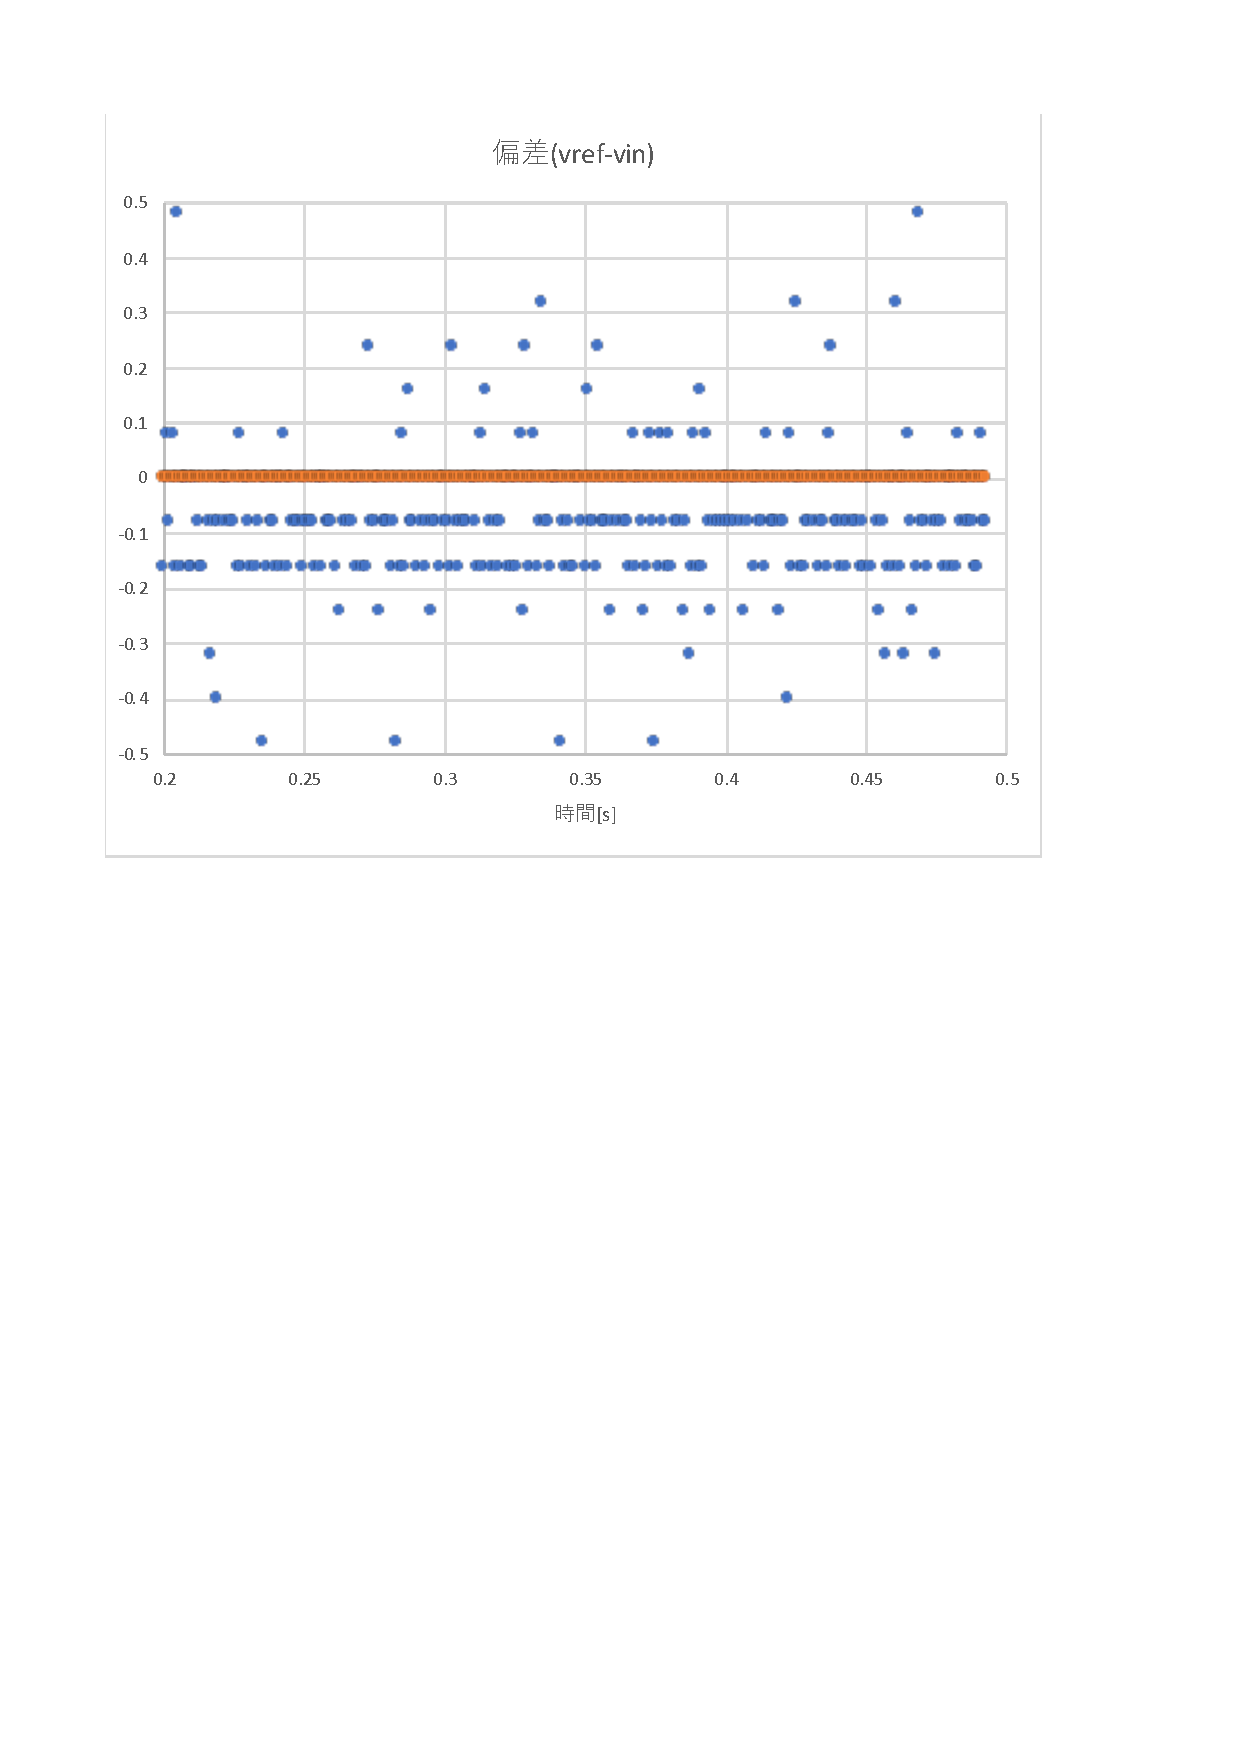
\includegraphics[width=9cm]{09in.pdf}
    \caption{制御回路(b)の位置制御}
    \label{09in}
\end{figure}

\begin{figure}[h]
    \centering
    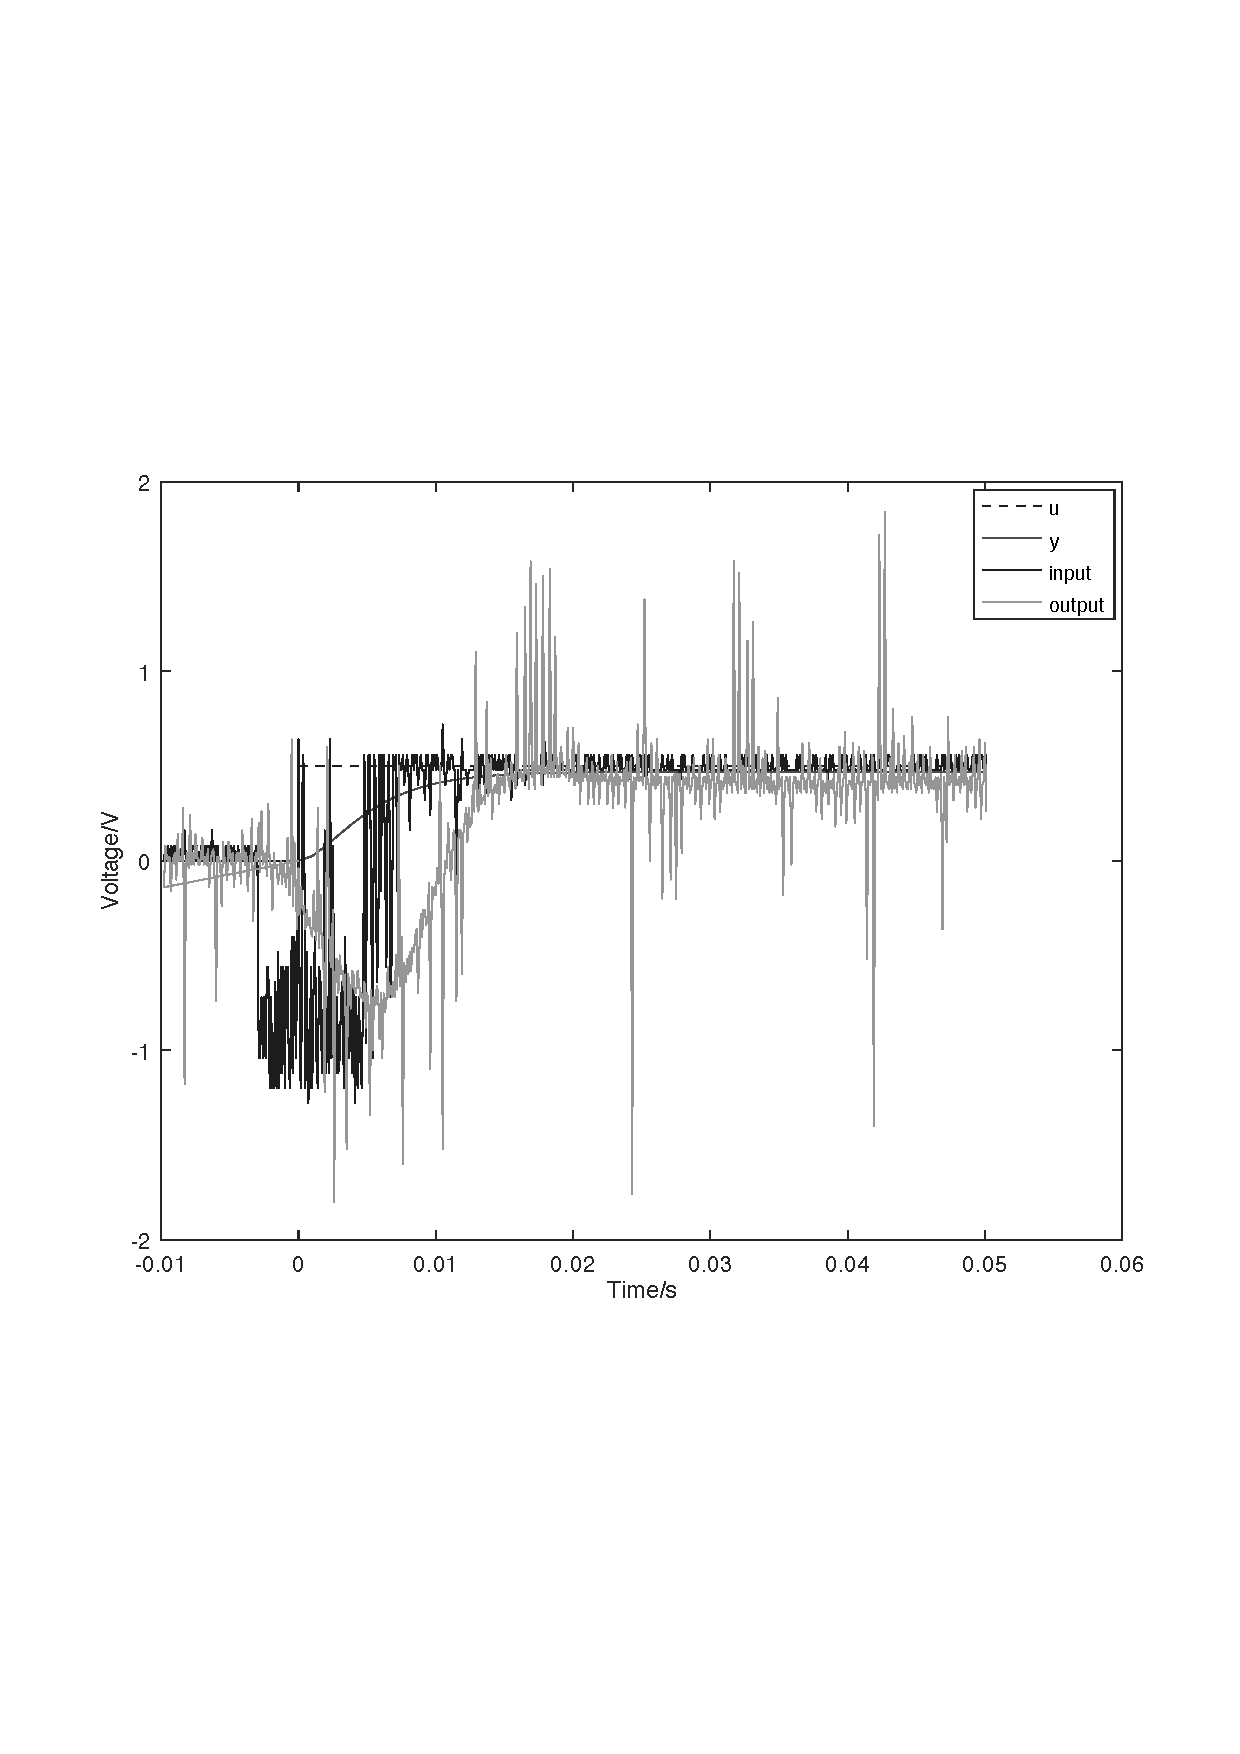
\includegraphics[width=9cm]{unitvain.pdf}
    \caption{(a)の速度制御のステップ応答$v_{\rm in}$}
    \label{unitvain}
\end{figure}

\begin{figure}[h]
    \centering
    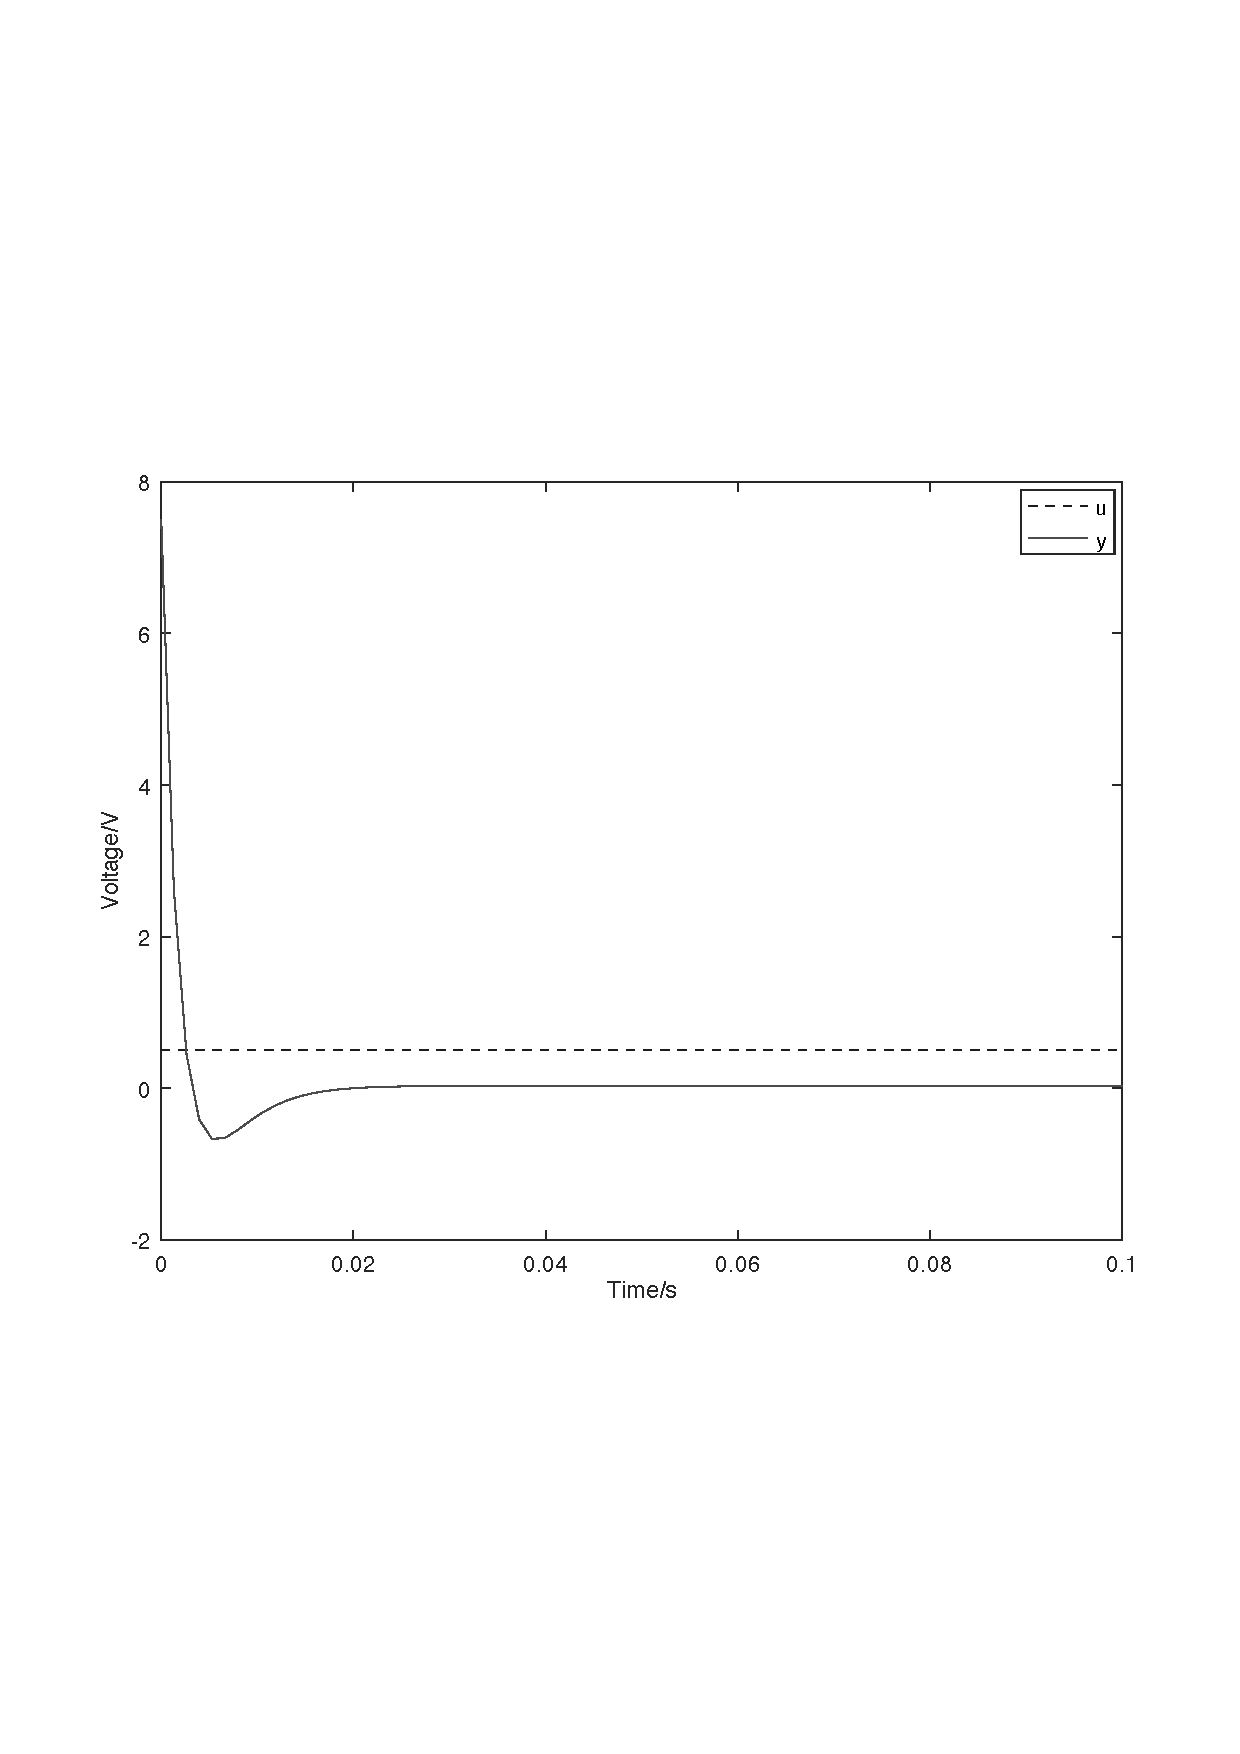
\includegraphics[width=9cm]{unitvaout.pdf}
    \caption{(a)の速度制御のステップ応答$v_{\rm out}$}
    \label{unitvaout}
\end{figure}

\begin{figure}[h]
    \centering
    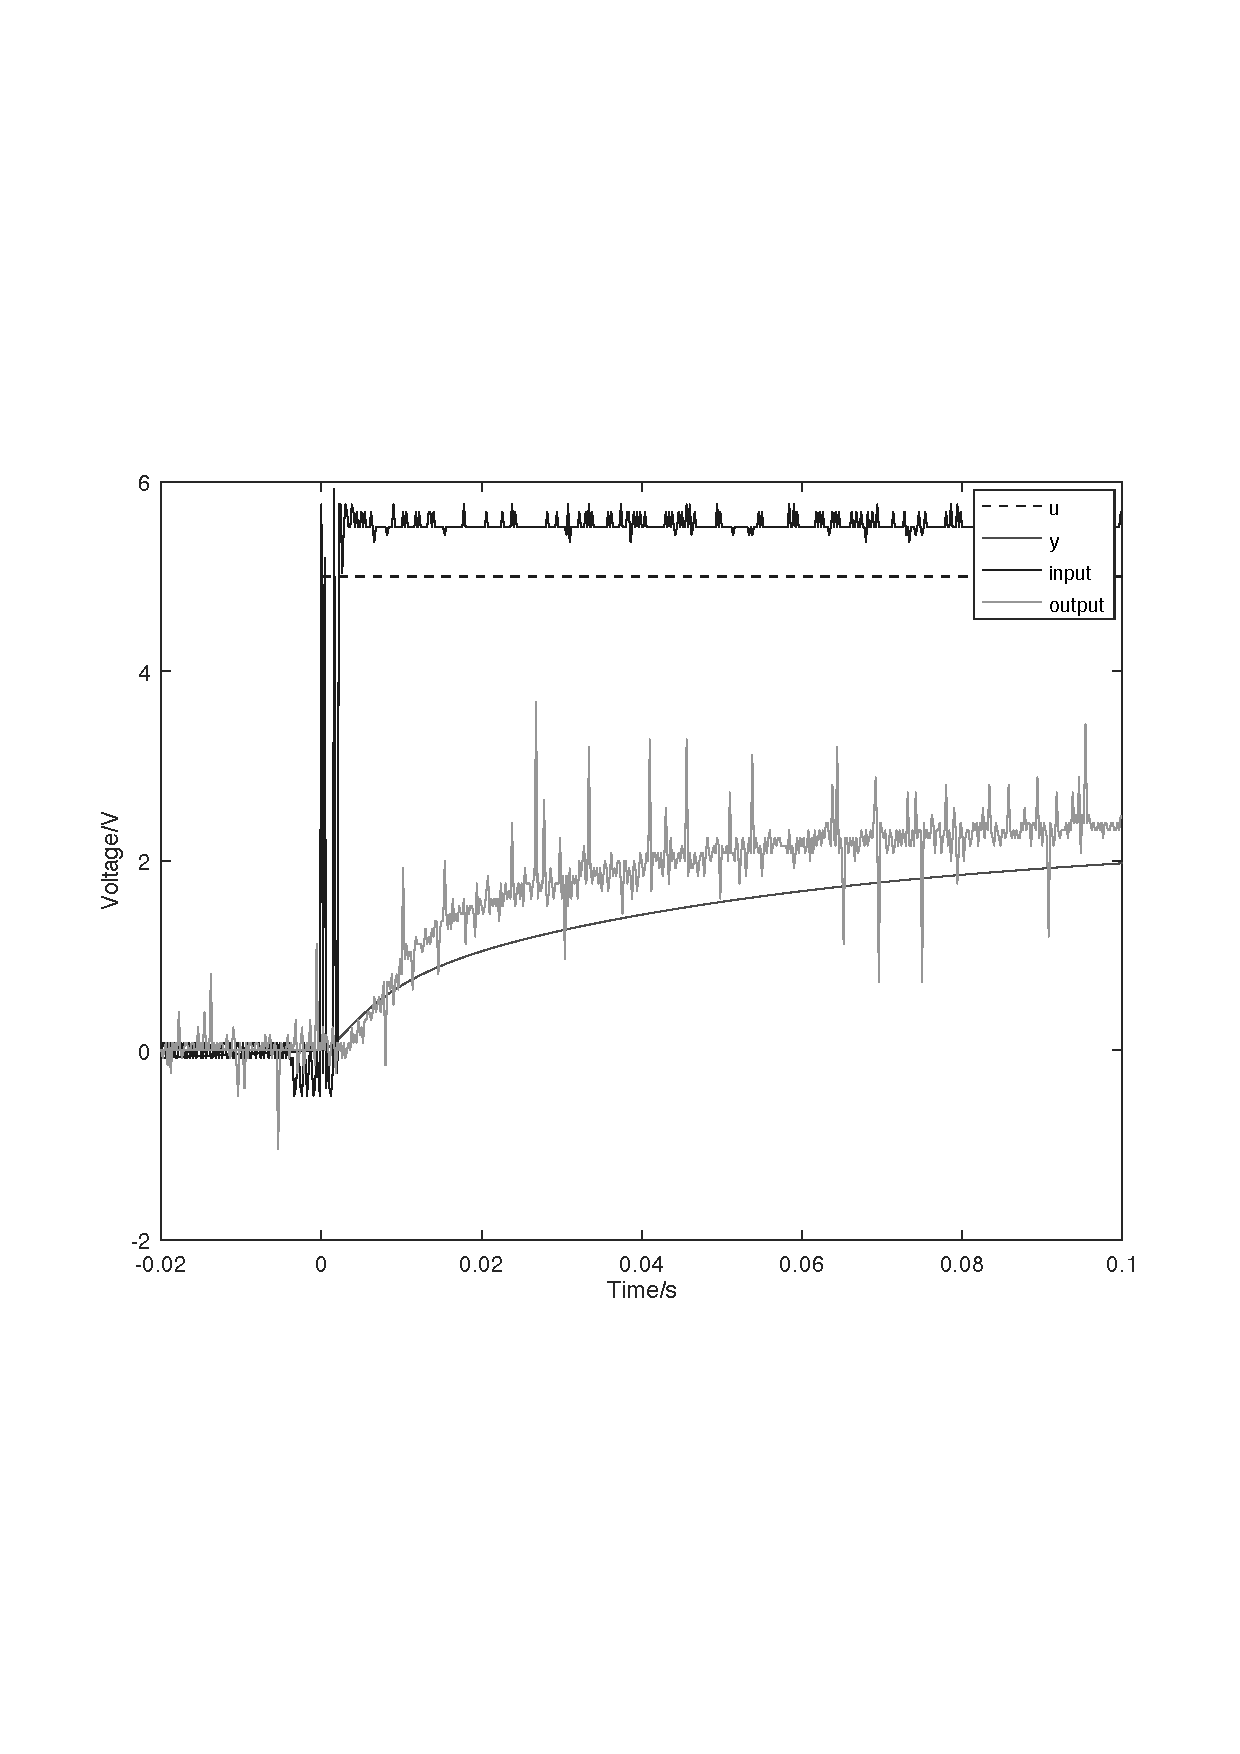
\includegraphics[width=9cm]{unitvbin.pdf}
    \caption{(b)の速度制御のステップ応答$v_{\rm in}$}
    \label{unitvbin}
\end{figure}

\begin{figure}[h]
    \centering
    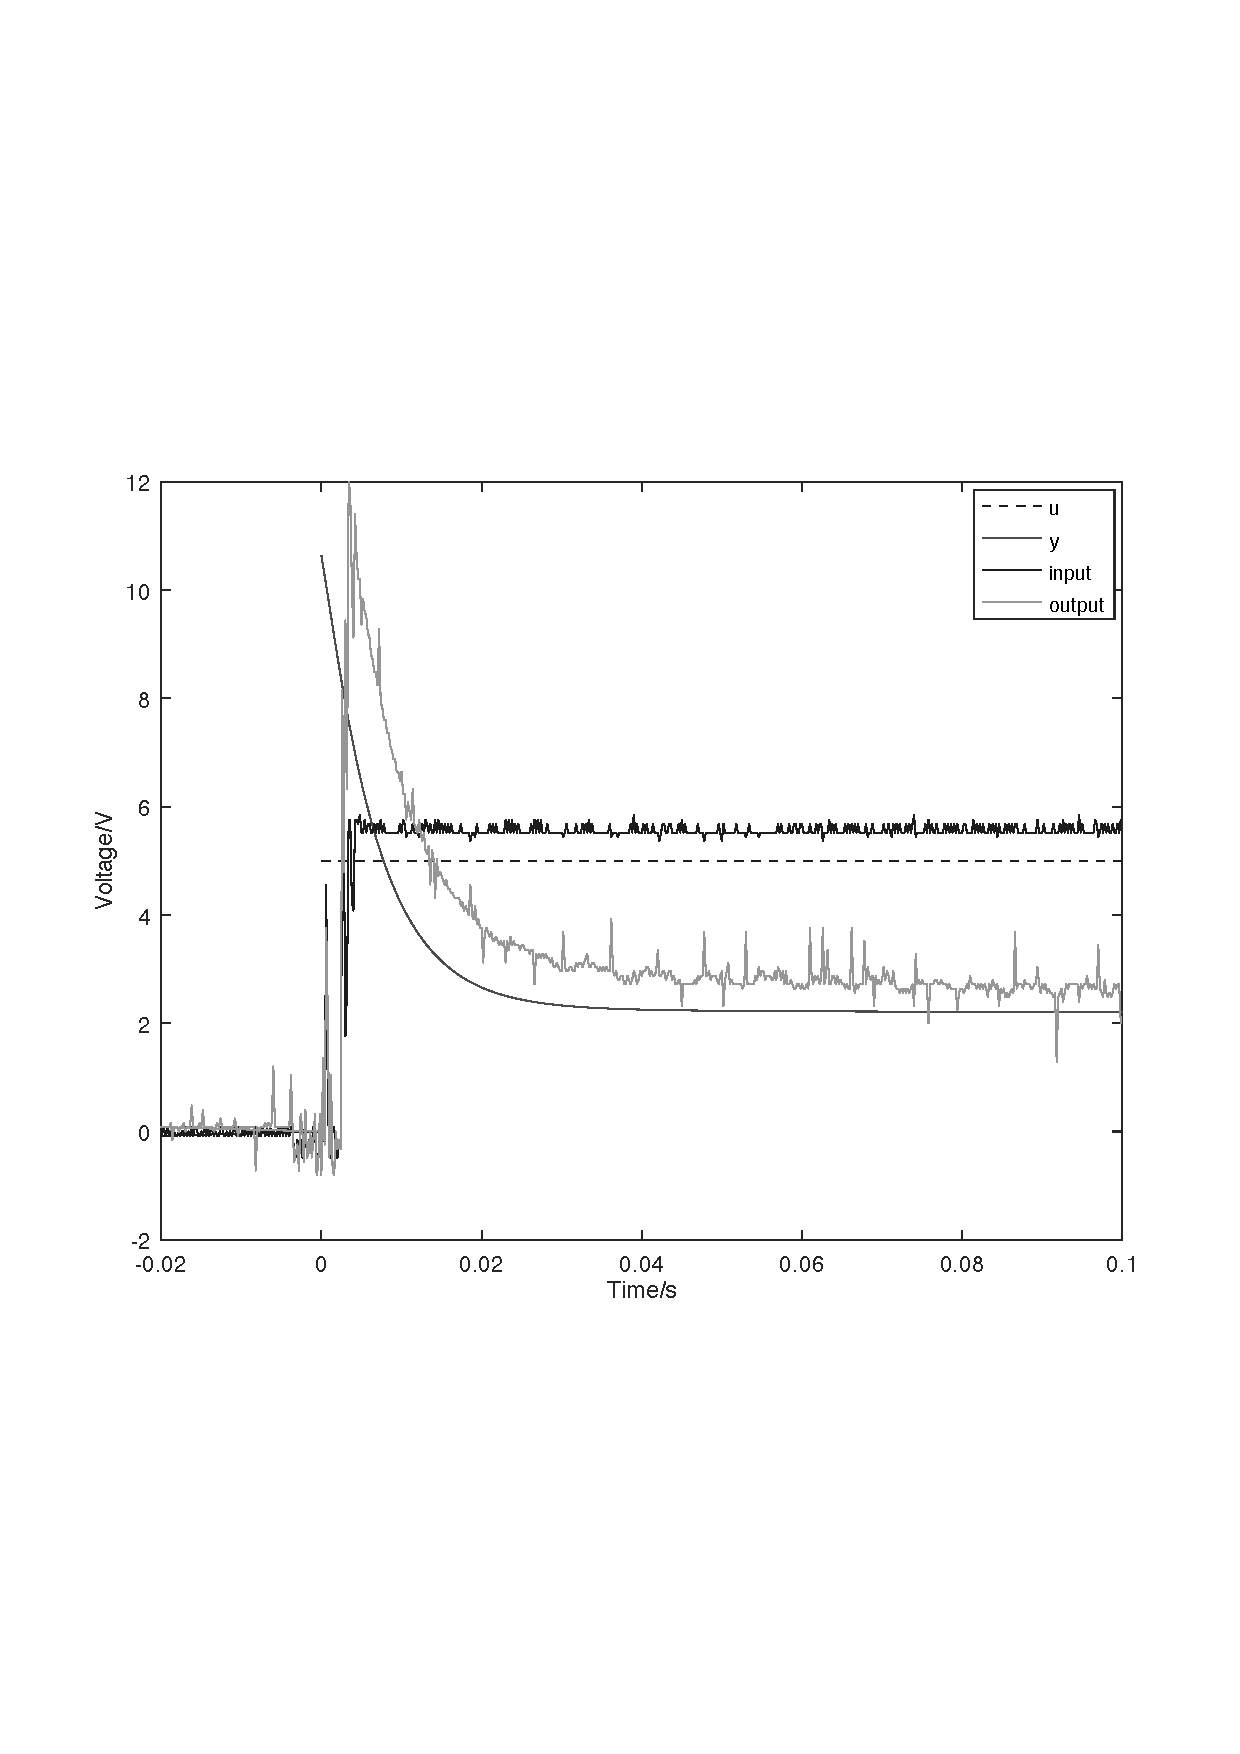
\includegraphics[width=9cm]{unitvbout.pdf}
    \caption{(b)の速度制御のステップ応答$v_{\rm out}$}
    \label{unitvbout}
\end{figure}

\begin{figure}[h]
    \centering
    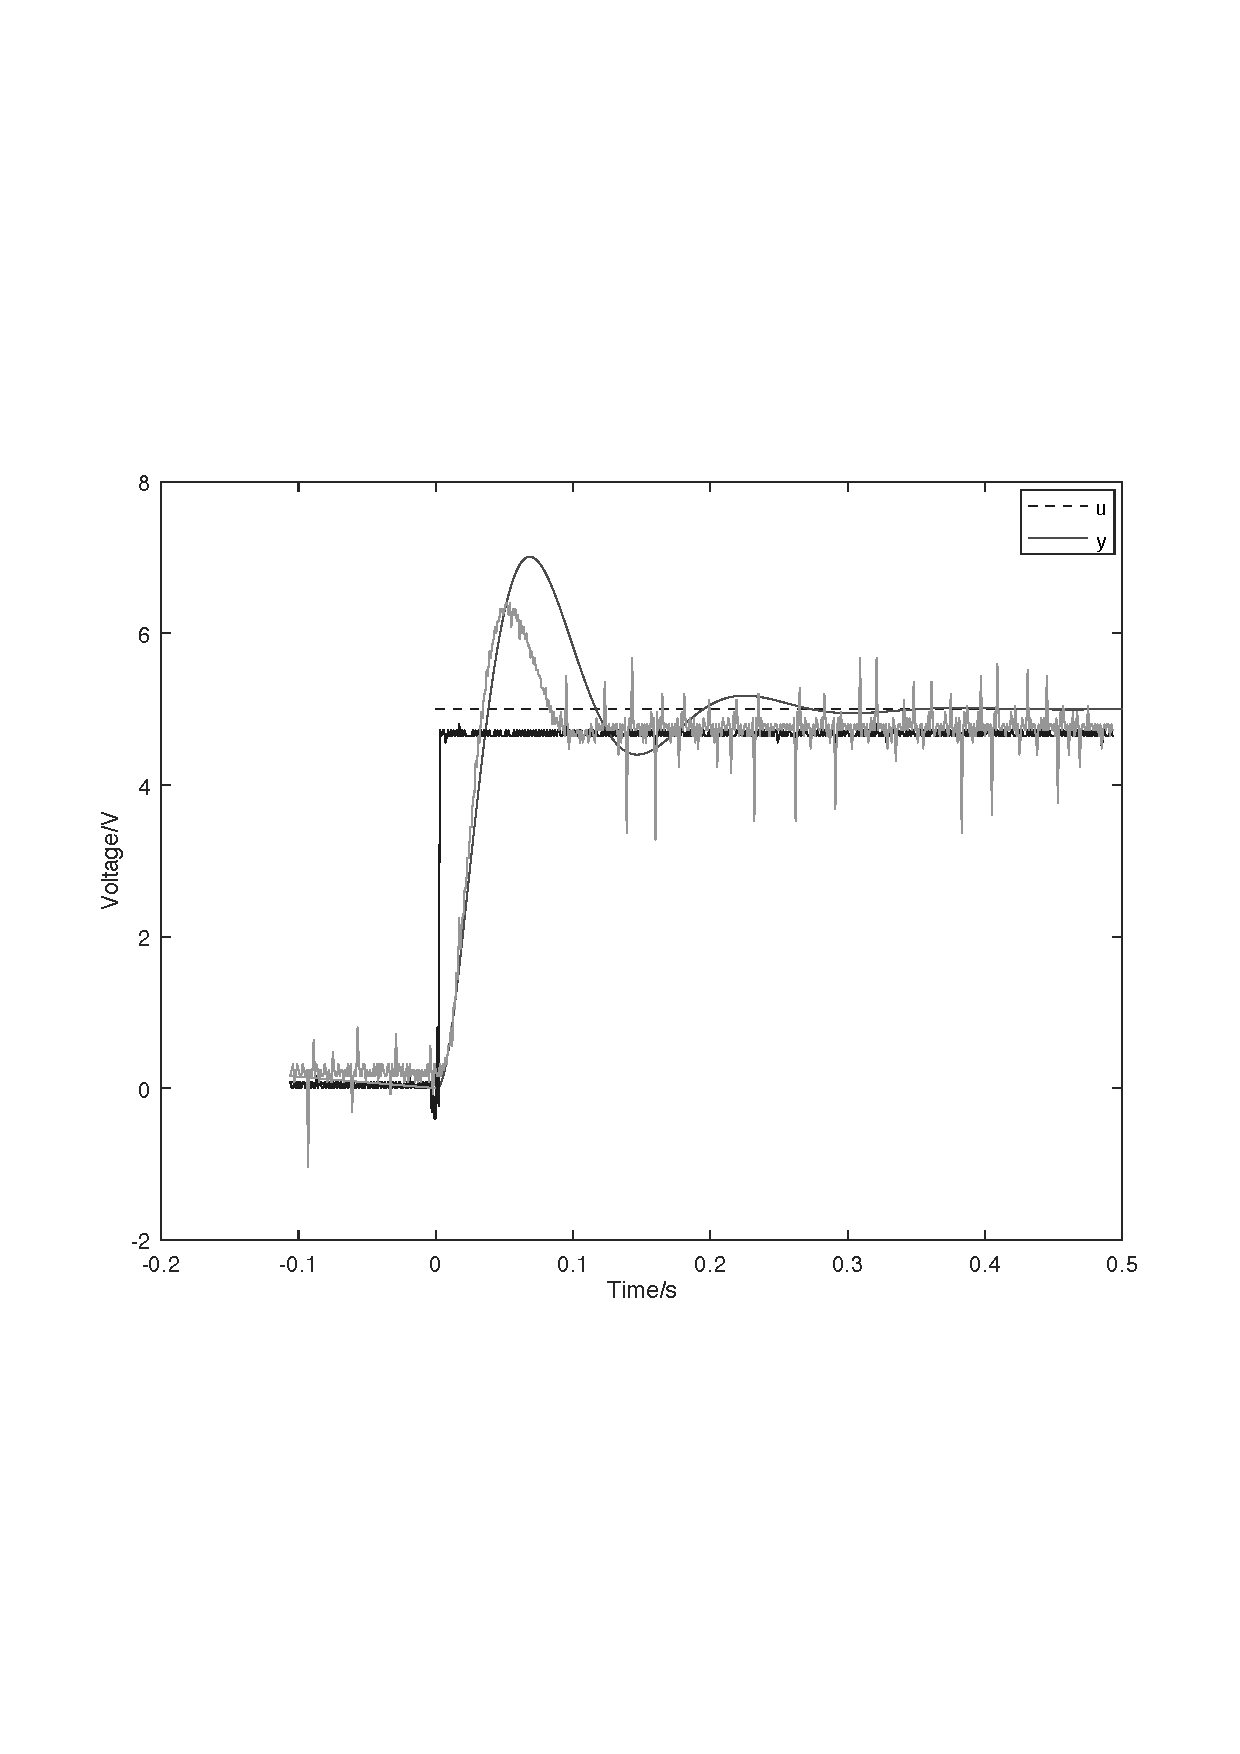
\includegraphics[width=9cm]{unitpbin.pdf}
    \caption{(b)の位置制御のステップ応答$v_{\rm in}$}
    \label{unitpbin}
\end{figure}

\begin{figure}[h]
    \centering
    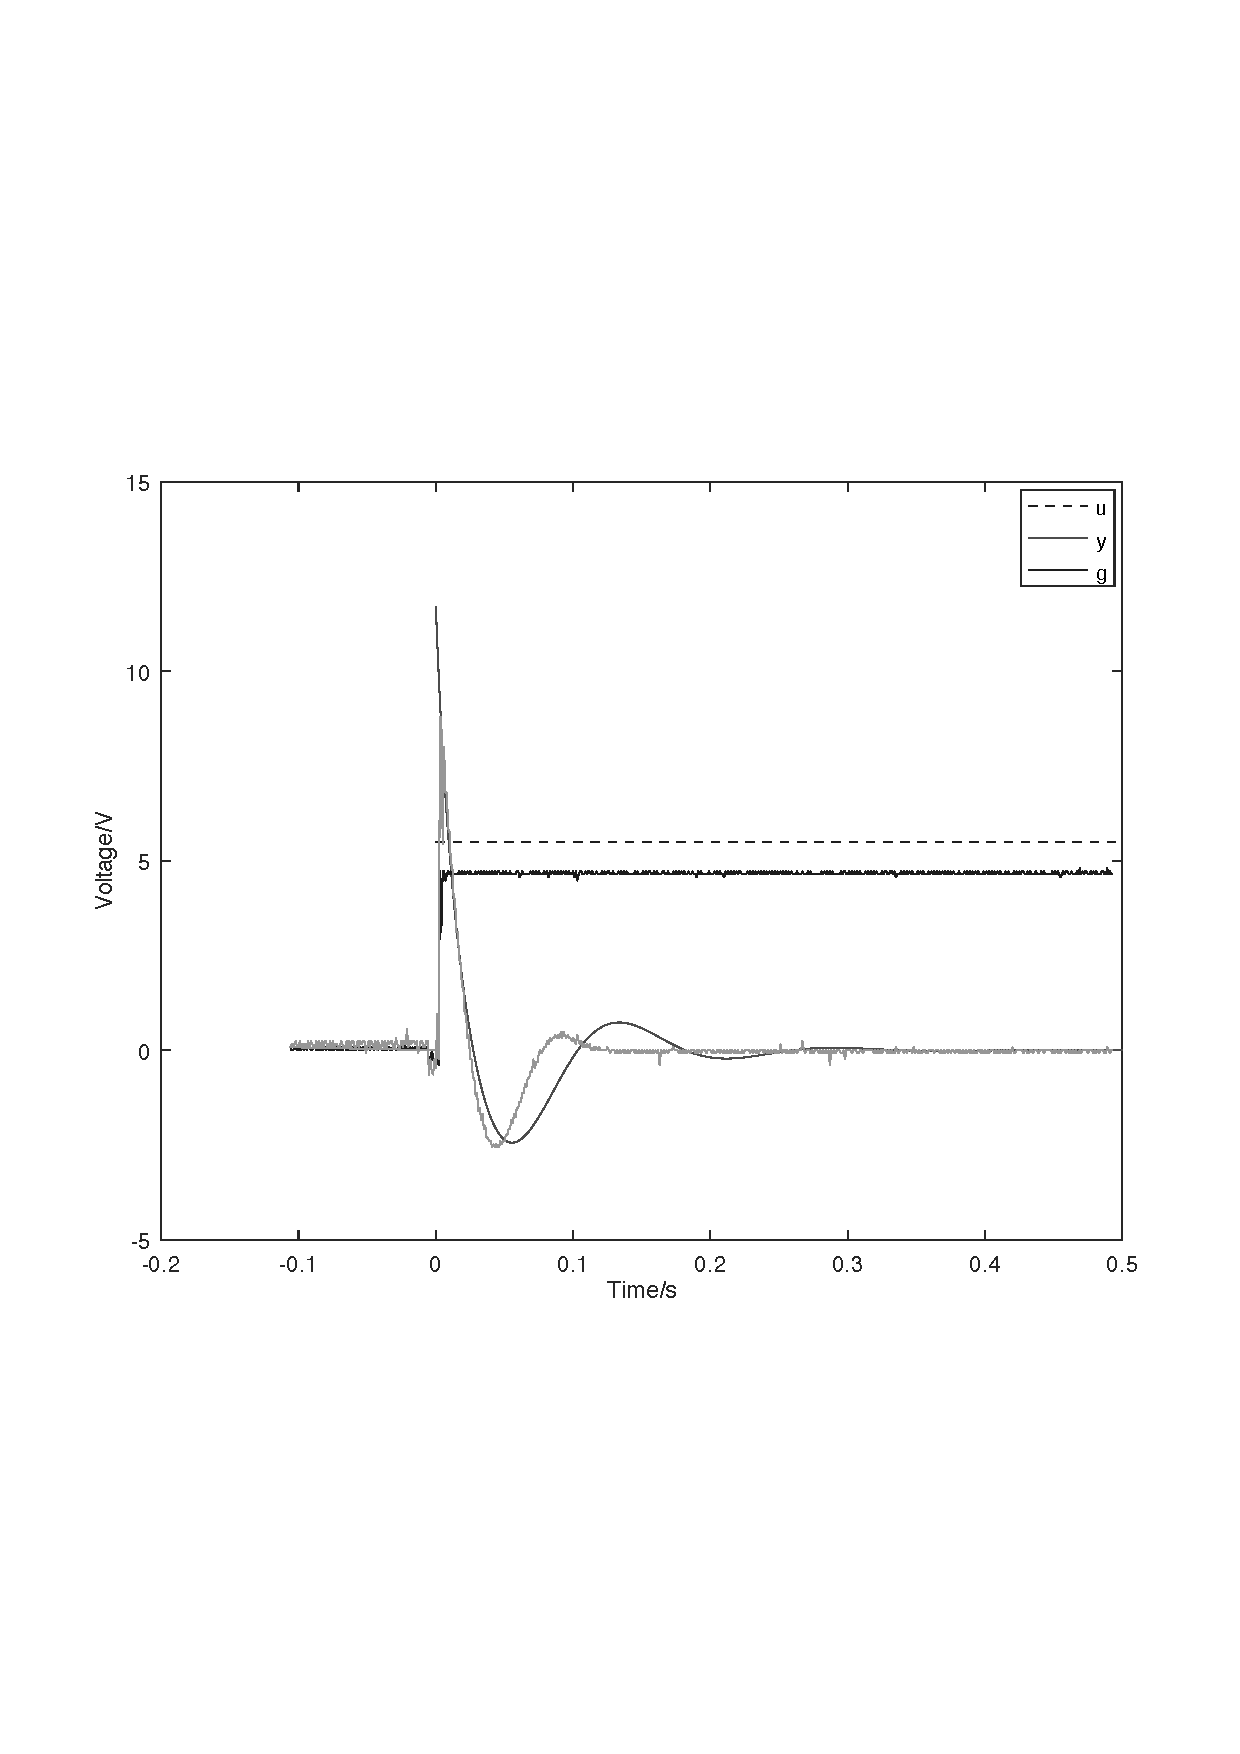
\includegraphics[width=9cm]{unitpvout.pdf}
    \caption{(b)の位置制御のステップ応答$v_{\rm out}$}
    \label{unitpbout}
\end{figure}

\newpage
\ 
\newpage
\ 
\newpage
\ 
\newpage
\ 
\newpage

\section{考察}

まず定常偏差の計算結果と実測値が制御回路(a)において一致が見られなかったのは、
目標値の設定電圧が低かったことが原因として考えられる。
比例ゲイン(a)では今回用いた素子により15倍のゲインが得られるものであったが、
オシロスコープの測定範囲を考慮して目標電圧が0.5Vを設定した。
したがって、電圧が低い分期待通りの制御ができなかったのだと考えた。

次にステップ応答の理論値と実測値の比較だが、
制御回路(a)の速度制御以外では、概ね理論値と実測値が一致している。
しかし、差動増幅器による速度制御では初めに電圧低下が起こったため、
理論値と実測値が一致していない。
これは、初めに高い電圧をかけた時に、モーターの慣性によって
逆向きに誘導された電流によって生じた逆向きの起電力なのではないかと考えた。
これは(b)においては間に挿入されたコンデンサによって緩和されて
いるのではないかとも考えた。

これを補填するために、Octave上で逆向きのステップ信号を
入力して理論値を計算し直したグラフを\ref{riron_new}、
そのためのコードをソースコード2に示す。
これにより理論値と実測値が近い結果になった。

\begin{figure}[h]
    \centering
    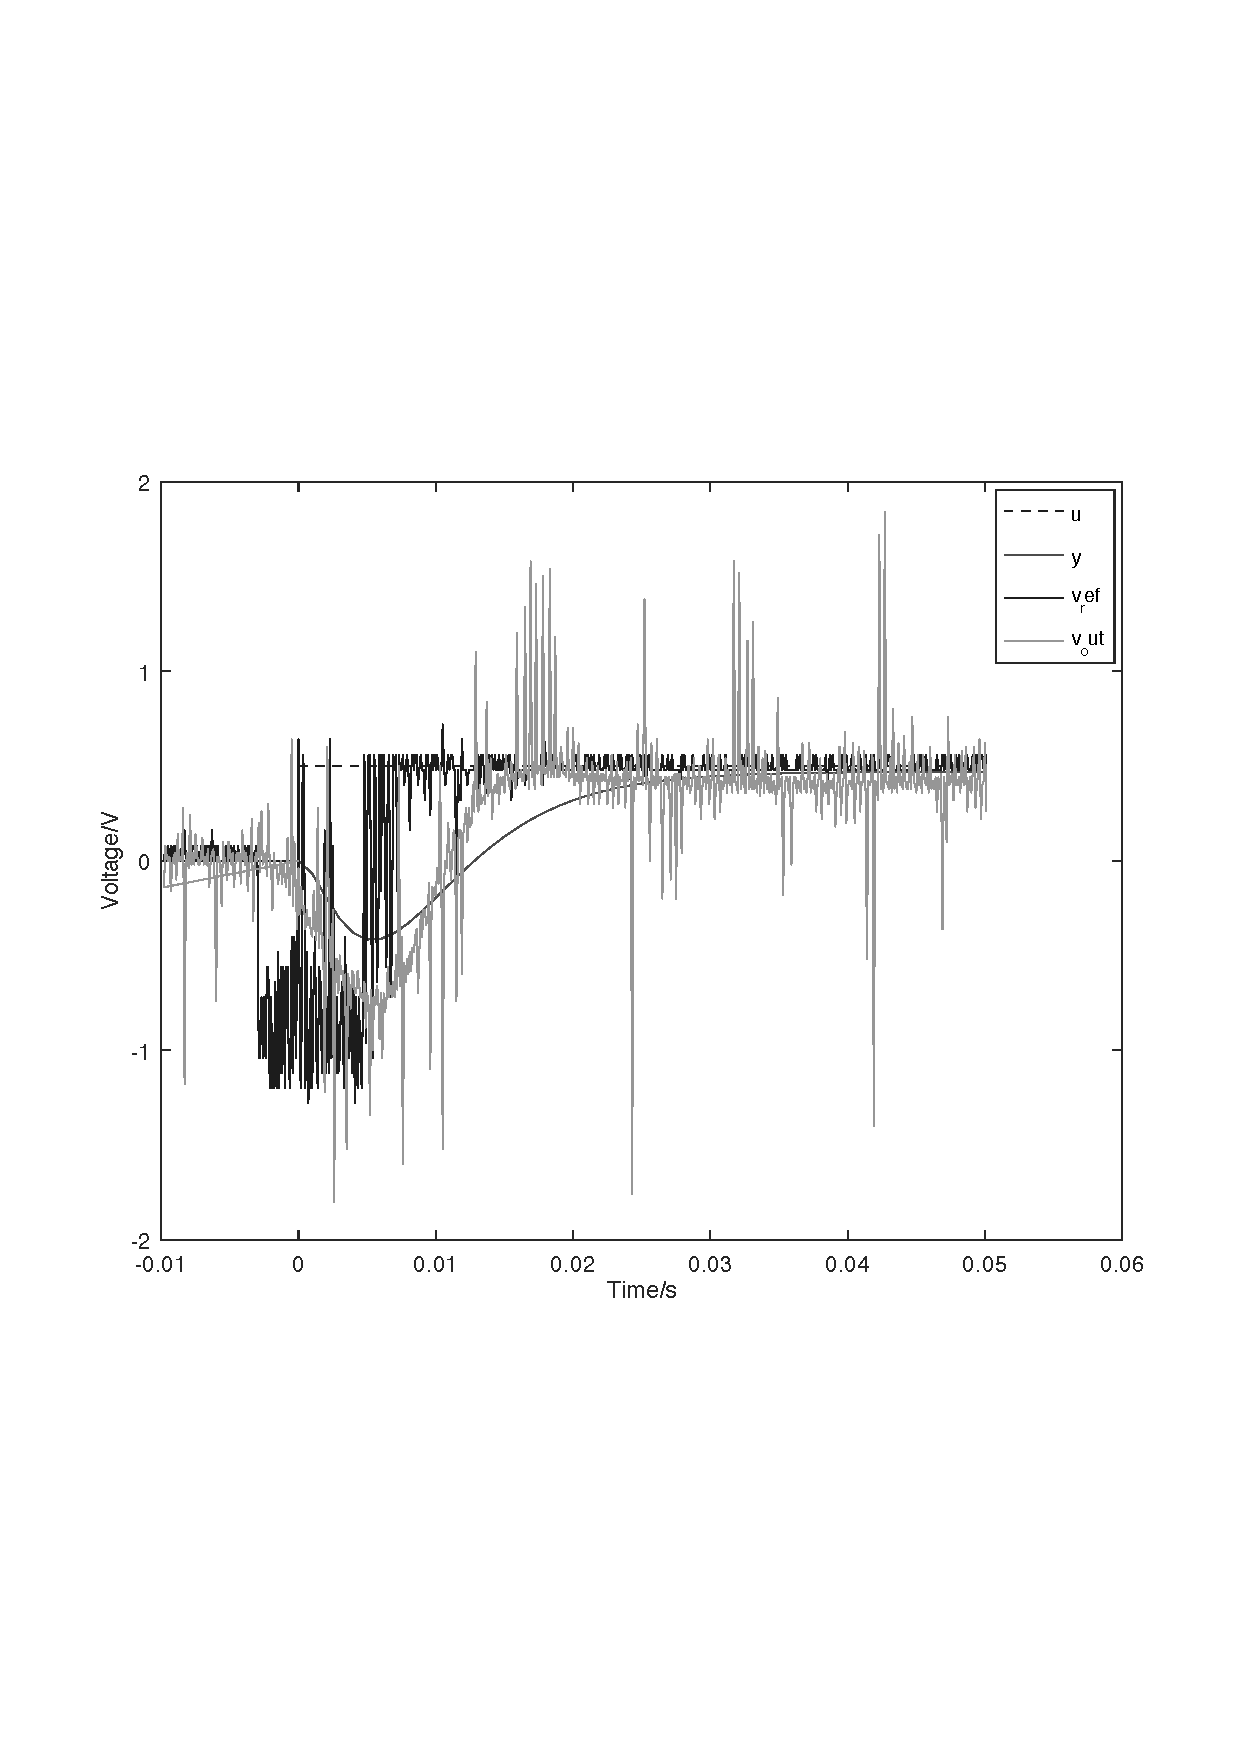
\includegraphics[width=9cm]{riron_new.pdf}
    \caption{入力を補填したステップ応答}
    \label{riron_new}
\end{figure}

\newpage

\begin{lstlisting}[caption={vain\_2.m}]
pkg load control;

clear;

R1=20e3;
R2=300e3;
K=1.03;
TE=1.3267e-3;
TM=0.0909;

A=csvread("1023__01in.csv");

L=0.010;
stepsize=0.5;

G=tf([K*R2], [R1*TE*TM R1*(TE+TM) R1+K*R2]);
G_neo=G*tf([-L/2,1], [L/2,1]);


[y_unit1 t]=step(G,0.05);
y1=y_unit1*stepsize*(-1);

[y_unit2 t]=step(G_neo,0.05);
y2=y_unit2*stepsize*2;

y=y1+y2;

u=ones(length(t),1)*stepsize;

figure
plot(t,u,'b--',t,y,'r-', 
    A(:,1), A(:,2), 'b-', A(:,1), A(:,3), 'g-')
legend('u','y', 'v_{ref}', 'v_{out}');
xlabel('Time/s');
ylabel('Voltage/V');
\end{lstlisting}

% 実験レポート3
% ここまで

% 参考文献
\newpage
\thispagestyle{empty}
\nocite{key1}
\nocite{key2}
\bibliographystyle{junsrt}
\bibliography{assets/ref}

\end{document}